\documentclass{article}

% Paquetes
\usepackage{arxiv}
\usepackage[utf8]{inputenc}
\usepackage[T1]{fontenc}
\usepackage[spanish,es-tabla]{babel}
\usepackage{lmodern}
\usepackage{hyperref}
\usepackage{url}
\usepackage{booktabs}
\usepackage{amsfonts}
\usepackage{nicefrac}
\usepackage{microtype}
\usepackage{graphicx}
\usepackage{adjustbox}
\usepackage{doi}
\usepackage{amsmath}
\usepackage{amssymb}
\usepackage{algorithm}
\usepackage{algpseudocode}
\usepackage{xcolor}
\usepackage{float}
\usepackage{placeins}
\usepackage{needspace}
\usepackage{etoolbox}

% Configuración
\hypersetup{
    pdftitle={Núcleo de Regulación Afectiva: Un marco de control homeostático para agentes de IA estables y seguros},
    pdfauthor={J. Eduardo Damián Reynoso},
    pdfkeywords={Computación Afectiva, Seguridad en IA, Control Homeostático, Aprendizaje por Refuerzo},
    hypertexnames=false,
    colorlinks=true,
    linkcolor=blue,
    citecolor=blue,
    urlcolor=blue
}

\title{Núcleo de Regulación Afectiva: Un marco de control homeostático para agentes de IA estables y seguros}

% Título abreviado para el encabezado
\renewcommand{\shorttitle}{\textsc{Núcleo de Regulación Afectiva (ARC)}}
\renewcommand{\headeright}{\textsc{Preimpreso (Versión en español)}}
\setcounter{topnumber}{3}
\setcounter{bottomnumber}{2}
\setcounter{totalnumber}{5}
\renewcommand{\topfraction}{0.9}
\renewcommand{\bottomfraction}{0.8}
\renewcommand{\textfraction}{0.07}
\renewcommand{\floatpagefraction}{0.8}
\raggedbottom
\linespread{1.09}\selectfont
\setlength{\textfloatsep}{18pt plus 4pt minus 3pt}
\setlength{\floatsep}{14pt plus 3pt minus 3pt}
\setlength{\intextsep}{16pt plus 4pt minus 3pt}
\setlength{\abovecaptionskip}{4pt}
\setlength{\belowcaptionskip}{11pt}
\setlength{\parskip}{7pt plus 1pt minus 1pt}
\setlength{\parindent}{0pt}
\clubpenalty=10000
\widowpenalty=10000
\displaywidowpenalty=10000
\makeatletter
\setlength{\@fptop}{8pt}
\setlength{\@fpsep}{12pt}
\setlength{\@fpbot}{0pt plus 1fil}
\makeatother
\newcommand{\scenarioheader}[1]{\Needspace{20\baselineskip}\textbf{Escenario: #1}}
\makeatletter
\pretocmd{\section}{\Needspace{14\baselineskip}}{}{}
\pretocmd{\subsection}{\Needspace{10\baselineskip}}{}{}
\pretocmd{\subsubsection}{\Needspace{7\baselineskip}}{}{}
\pretocmd{\paragraph}{\Needspace{6\baselineskip}}{}{}
\makeatother

% Autor: apellido paterno "Damián" (primer apellido), "Reynoso" es el apellido
% materno según la convención hispana. Las llaves indican a LaTeX/BibTeX que
% "Damián Reynoso" es un apellido compuesto, de modo que las citas cortas
% se rindan como "Damián Reynoso 2026" y las formas abreviadas elijan "Damián".
\author{
  J. Eduardo {Dami\'{a}n Reynoso} \\
  Investigador Independiente, M\'{e}xico \\
  \texttt{edamianreynoso@gmail.com} \\
  ORCID: \href{https://orcid.org/0009-0008-6544-328X}{0009-0008-6544-328X}
}

\date{Febrero 2026}

\begin{document}

\maketitle

\begin{abstract}
A medida que los agentes de IA se vuelven más sofisticados, existe un interés creciente en dotarlos de representaciones de estado interno análogas a estados afectivos. Sin embargo, los estados afectivos sin regulación pueden derivar en inestabilidad, bucles perseverativos (rumiación) y vulnerabilidad a la manipulación. Presentamos el \textbf{Núcleo de Regulación Afectiva (ARC, Affective Regulation Core)}, un marco de control inspirado en funciones de la corteza prefrontal que mantiene la estabilidad en agentes con estados afectivos internos. También presentamos el \textbf{Benchmark de Estabilidad y Seguridad Afectiva (ASSB, Affective Stability \& Safety Benchmark)}, un protocolo de evaluación reproducible con métricas para tiempo de recuperación, índice de rumiación y esfuerzo de control.

Nuestros experimentos abarcan 6 líneas de investigación y \textbf{15 arquitecturas de controlador} (incluyendo variantes P, PID, LQR, LQI, jerárquicas, meta-control, H$\infty$ robustas y adaptativas), demostrando que:
\begin{enumerate}
    \item Las dinámicas afectivas no controladas colapsan bajo perturbación (PerfMean $\leq$ 0.30 en escenarios de estabilidad), mientras que ARC mantiene PerfMean $\geq$ 0.93 a lo largo del conjunto L1--L5 completo; específicamente en escenarios L1 de estabilidad, la configuración de referencia \texttt{arc\_v1} alcanza \textbf{0.966} (vs.\ 0.297 del baseline). \textbf{Las variantes de ARC con acción anti-rumiación explícita} (supresión de DMN en \texttt{arc\_v1}, acción integral en PID / LQI / MPC+LQI, o el diseño H$\infty$ robusto) \textbf{llevan el Índice de Rumiación exactamente a 0.00 en L1} (cero pasos sobre $s_{\text{rum}\tau}$; Tablas~\ref{tab:l1_results},~\ref{tab:significance}). Las variantes LQR puras (\texttt{arc\_v1\_lqr}, \texttt{arc\_v3\_lqr\_meta}) y la variante LQR-jerárquica (\texttt{arc\_v2\_hier}) \emph{no} apuntan al umbral de rumiación y, en consecuencia, pueden exhibir RI $>1$ en escenarios L1 (ej.\ RI $\approx 1.38$--$1.41$ en \texttt{reward\_flip}; Tabla~\ref{tab:g1_reward_flip}): esto es una consecuencia esperada de minimizar el error cuadrático del estado en lugar de las excursiones del umbral, no un modo de falla, y es una motivación para preferir arquitecturas no-LQR cuando la supresión de rumiación es el objetivo primario. \textbf{Los controladores con acción integral (PID, LQI, MPC+LQI) además mantienen RI $= 0$ globalmente a lo largo de L1--L5}, mientras que el \texttt{arc\_v1} proporcional se asienta en RI $\approx 0.15$ al agregar sobre los 10 escenarios L1--L5 (Tabla~\ref{tab:controller_comparison}; media por-escenario $0.148$).
    \item El meta-control ARC reduce el esfuerzo de control agregado en un \textbf{20.9\%} (de $0.777$ a $0.615$ en el agregado de 10 escenarios) con una pequeña ganancia de desempeño ($+0.7\%$); reportamos esto como un efecto direccional (sin test paramétrico de significancia; véase Sección~\ref{sec:statistical_analysis}).
    \item \textbf{Los controladores H$\infty$ Robustos} son la única variante ARC que satisface simultáneamente las tres condiciones: PerfMean $\geq 0.93$ en L1--L3, RI $= 0$ a lo largo de L1--L5 \emph{incluyendo} adversarial coupling, y ningún colapso por debajo del baseline no controlado en ningún escenario (Tabla~\ref{tab:controller_comparison}); bajo este test de tres criterios son la arquitectura más consistente del conjunto. En contraste, los controladores integrales (PID, LQI, MPC+LQI) colapsan por debajo del desempeño del baseline bajo adversarial coupling debido al windup del integrador---un hallazgo negativo importante que reportamos transparentemente y analizamos en detalle.
    \item En aprendizaje por refuerzo tabular sobre \texttt{ChangingGoalGridWorld}, el \textbf{componente de memory-gating de ARC solo} es el mecanismo individual más fuerte, alcanzando 71.8\% de éxito (\textbf{+79.9\%} relativo al baseline de 39.9\%); el wrapper ARC-RL integrado que combina memory gating con detección de cambio alcanza 59.8\% (+49.8\% sobre el baseline), indicando que los dos mecanismos, aunque individualmente beneficiosos, interactúan sub-aditivamente al componerlos --- un hallazgo que discutimos como una limitación de la integración actual (Sección~7.4) más que como una validación del wrapper completo. Experimentos preliminares con Deep RL (DQN) tienen bajo desempeño e indican que los aprendices basados en gradiente requieren rediseño arquitectónico---reportado explícitamente en el Apéndice~\ref{sec:dqn_suite} como un límite de alcance y motivación para trabajo futuro.
\end{enumerate}

Todo el código y los datos están disponibles en \url{https://github.com/edamianreynoso/arc-assb-controller} (tag \texttt{arc-paper-v1}); véase el Apéndice~A para la especificación completa del entorno (versión de Python, mínimos de librerías, perfil de hardware, lista canónica de semillas) y el anclaje de hash de commit para este envío.
\end{abstract}

\keywords{Regulación afectiva \and Control homeostático de agentes de IA \and Seguridad del estado interno \and Benchmarks de rumiación \and Windup integral \and Control robusto H$\infty$ \and Supresión de la red neuronal por defecto \and Benchmark ASSB}

\section{Introducción}

\subsection{Motivación}

Los sistemas de IA modernos incorporan cada vez más representaciones de estado interno que van más allá del desempeño en tareas---incluyendo señales afectivas que priorizan el aprendizaje, modulan la memoria y señalan necesidades internas \cite{Damasio1994, Picard1997}. Sin embargo, los estados afectivos introducen riesgos: sin una regulación apropiada, pueden causar inestabilidad, bucles perseverativos (funcionalmente análogos a la rumiación) y susceptibilidad a la manipulación \cite{Amodei2016}.

Este artículo aborda una pregunta fundamental: \textbf{Si un agente tiene estados afectivos internos, ¿qué mecanismos de control son necesarios para mantener la estabilidad y la recuperabilidad bajo perturbación?}

\subsection{Contribuciones}

\begin{enumerate}
    \item \textbf{Un modelo de espacio de estados de 10 dimensiones} de un agente con componentes cognitivos, afectivos y narrativos integrados (Sección 3).
    \item \textbf{El Núcleo de Regulación Afectiva (ARC)}, una familia de 15 arquitecturas de controlador que incluye variantes P, PID, LQR, LQI, jerárquicas, meta-control, H$\infty$ robustas y MPC (Sección 4).
    \item \textbf{El Benchmark de Estabilidad y Seguridad Afectiva (ASSB)}, con escenarios y métricas reproducibles (Sección 5).
    \item \textbf{Una escalera de validación guiada por hipótesis (H1--H6)} que mapea líneas de investigación a modos de falla y métricas medibles (Sección 5.3).
    \item \textbf{Validación exhaustiva} a lo largo de 6 líneas de investigación, 15 arquitecturas de controlador e integración con RL tabular (Sección~6). Reportamos transparentemente tanto hallazgos positivos (las propiedades de estabilidad y anti-rumiación de ARC) como negativos (el colapso por windup integral bajo adversarial coupling; el bajo desempeño del DQN modulado por ARC en benchmarks de deep-RL). Estos últimos delimitan el alcance y motivan el programa de trabajo futuro de la Sección~7.5.
\end{enumerate}

\subsection{Alcance}

No afirmamos que nuestro modelo capture toda la complejidad de la emoción humana ni su fenomenología. Tratamos las variables internas (arousal, valencia, intensidad narrativa) \textbf{estrictamente como señales funcionales} que modulan el procesamiento y la priorización. Cualquier uso de términos como ``afecto'', ``rumiación'' o ``ansiedad'' se refiere a estas dinámicas funcionales dentro del sistema de control, no a experiencia biológica o consciente. Nuestra contribución es demostrar que tales estados funcionales requieren mecanismos de control explícitos para permanecer estables. Por último, nuestras dinámicas de estado están diseñadas para plausibilidad funcional más que para fidelidad biológica, y el análisis formal de estabilidad (p.\ ej., pruebas de Lyapunov) queda como trabajo futuro. La validación actual se basa en la experimentación empírica en un amplio rango de condiciones.

\section{Trabajo Relacionado}

\subsection{Computación Afectiva}

La computación afectiva se enfoca en el reconocimiento, síntesis y simulación de emociones \cite{Picard1997, Scherer2010}. Muchos sistemas operacionalizan el afecto en representaciones de baja dimensión (p.\ ej., valencia y arousal) \cite{Russell1980}. La mayoría del trabajo aborda la expresión externa más que la regulación interna. Nuestro trabajo aborda el \textit{problema de control} para estados internos.

\subsection{Emoción en Aprendizaje por Refuerzo}

Trabajos recientes usan señales tipo-emoción como modulación del refuerzo o exploración \cite{Moerland2018}. Direcciones relacionadas estudian cómo variables fisiológicas/homeostáticas pueden incrustarse en objetivos de RL \cite{Keramati2014}, y cómo las restricciones y objetivos de seguridad pueden imponerse en sistemas de aprendizaje \cite{Garcia2015}. En RL seguro, estos objetivos se formalizan típicamente como Procesos de Decisión de Markov Restringidos (CMDP) \cite{Altman1999} y se abordan con métodos de optimización de políticas restringidas \cite{Achiam2017}. Suites externas de benchmarks de seguridad como AI Safety Gridworlds \cite{Leike2017}, Safety Gym \cite{Ray2019} y Safety-Gymnasium \cite{Ji2023} motivan protocolos de evaluación estandarizados, y revisiones recientes sistematizan las formulaciones de restricciones \cite{Wachi2024}. Sin embargo, estos enfoques típicamente carecen de:
\begin{itemize}
    \item Regulación homeostática con umbrales de seguridad
    \item Mecanismos anti-rumiación (control de DMN)
    \item Memory gating bajo estrés
    \item Benchmarks dirigidos a dinámicas de estabilidad interna (recuperación, rumiación, esfuerzo)
\end{itemize}

\subsection{Regulación Emocional, Rumiación y la Red Neuronal por Defecto}

ARC está directamente inspirado en mecanismos de regulación emocional cognitiva comúnmente atribuidos al control prefrontal \cite{Ochsner2005}. Más ampliamente, la auto-regulación se ha descrito como bucles de retroalimentación que reducen discrepancias \cite{Carver1982}, y la regulación emocional es un campo maduro con modelos a nivel de proceso y de estrategia \cite{Gross1998}. En teoría de control, el problema de mantener excitación suficiente para la identificación de parámetros se conoce como \textbf{persistencia de excitación} \cite{Astrom2008}, una limitación central del control adaptativo en entornos de baja varianza (``benignos'').
En humanos, el procesamiento auto-referencial desregulado y la red neuronal por defecto (DMN, Default Mode Network) se han vinculado con dinámicas tipo-rumiación \cite{Raichle2001, Buckner2008, Hamilton2015}. Usamos la intensidad narrativa inspirada en DMN como proxy de ingeniería para la presión de perseveración.

\subsection{Posicionamiento de ARC}

Posicionamos a ARC como un enfoque \textit{de regulación primero}: el afecto se trata como un sistema dinámico interno que requiere control explícito. La mayoría de los enfoques de emoción en RL usan señales tipo-afecto principalmente como moduladores del aprendizaje/exploración más que como garantías de estabilidad.

\begin{table}[htbp]
\centering
\caption{Comparación de enfoques de regulación emocional}
\label{tab:comparison}
\begin{tabular}{@{}lcc@{}}
\toprule
Característica & Emoción en agentes RL \cite{Moerland2018} & \textbf{ARC} \\ \midrule
Regulación del estado interno & Parcial & Sí \\
Anti-rumiación (supresión DMN) & No & Sí \\
Memory gating bajo estrés & No & Sí \\
Meta-control / ajuste de ganancia & Parcial & Sí \\
Pruebas adversariales de seguridad & No & Sí \\
Integración con RL & Sí & Sí \\ \bottomrule
\end{tabular}
\end{table}

\textit{Criterios de clasificación (cualitativos, basados en los métodos revisados en \cite{Moerland2018}).} ``Sí'' = la característica se implementa como un mecanismo explícito de lazo cerrado con una acción medible sobre el estado interno del agente; ``Parcial'' = la característica aparece en al menos un método revisado pero como una modulación de lazo abierto (p.\ ej.\ un afecto escalar que influye en la exploración o la tasa de aprendizaje) sin un objetivo de regulación o señal de error explícita; ``No'' = no está presente en ningún método revisado. La comparación no es un enfrentamiento por-método, sino un resumen a nivel de categoría de los mecanismos revisados en la referencia; métodos individuales en \cite{Moerland2018} pueden implementar subconjuntos de manera diferente.

No reimplementamos cada método previo; en su lugar, comparamos contra baselines internos que aíslan la contribución de cada mecanismo (Sección 6.1).

A diferencia de los enfoques de RL homeostático que incrustan impulsos/variables internas dentro de la recompensa o del objetivo de aprendizaje \cite{Keramati2014}, ARC trata las variables tipo-afecto como un sistema dinámico interno explícito bajo control de lazo cerrado, permitiendo análisis de estabilidad/robustez y comparación sistemática entre familias de controladores. Complementando los benchmarks de RL seguro que evalúan principalmente el cumplimiento de restricciones ambientales externas \cite{Leike2017, Ray2019, Ji2023}, ASSB apunta a dinámicas internas relevantes para la seguridad---tiempo de recuperación, índice de rumiación y esfuerzo de control---bajo perturbaciones controladas. Hasta donde sabemos, no existe un benchmark estandarizado dedicado específicamente a la ``estabilidad afectiva'' en este sentido; se propone ASSB para llenar ese vacío. También distinguimos ARC de los controladores bio-inspirados de ``aprendizaje emocional'' como BELBIC, que usan mecanismos inspirados en emociones para controlar plantas físicas, no para regular los estados internos de un agente \cite{Lucas2004}. Finalmente, ARC aquí se refiere al Núcleo de Regulación Afectiva (Affective Regulation Core) y no debe confundirse con otros usos del acrónimo en contextos clínicos.

\section{Modelo}

\subsection{Espacio de Estados}

Definimos un vector de estado interno normalizado:

\begin{equation}
\mathbf{x}(t) = [\Phi, G, P, I, S, V, A, M_f, M_s, U]
\end{equation}

\begin{table}[htbp]
\centering
\caption{Variables de estado}
\label{tab:state_variables}
\begin{tabular}{@{}llc@{}}
\toprule
Variable & Descripción & Rango \\ \midrule
$\Phi$ & Proxy de integración (IIT) & [0, 1] \\
$G$ & Accesibilidad al workspace global & [0, 1] \\
$P$ & Precisión predictiva & [0, 1] \\
$I$ & Atención introspectiva & [0, 1] \\
$S$ & Intensidad narrativa (proxy DMN) & [0, 1] \\
$V$ & Valencia & [0, 1] \\
$A$ & Arousal & [0, 1] \\
$M_f, M_s$ & Memoria rápida/lenta & [0, 1] \\
$U$ & Incertidumbre & [0, 1] \\ \bottomrule
\end{tabular}
\end{table}

Interpretamos $\Phi$ como un proxy de integración inspirado en IIT \cite{Tononi2008}, $G$ como accesibilidad al workspace global \cite{Baars1988} y $P$ como precisión predictiva \cite{Friston2010}. Se usan como variables latentes relevantes para el control, no como afirmaciones sobre la conciencia humana.

\subsection{Capacidad Cognitiva}

Siguiendo una integración multiplicativa:

\begin{equation}
C_{cog}(t) = \Phi(t) \cdot G(t) \cdot P(t) \cdot I(t)
\end{equation}

Esto captura que el procesamiento consciente requiere que \textit{todos} los componentes estén funcionales.

\subsection{Función de Desempeño}

Antes de enunciar la función de desempeño, definimos dos umbrales que aparecen en ella. $a_{safe}$ y $s_{safe}$ son parámetros escalares en $[0,1]$ que delimitan la \emph{región de operación segura} para arousal e intensidad narrativa, respectivamente: cualquier valor por encima del umbral se penaliza en la función de desempeño (como $[A-a_{safe}]^+$, $[S-s_{safe}]^+$). Los valores por defecto son $a_{safe}=0.60$ y $s_{safe}=0.55$, guiados por la ley de Yerkes--Dodson (relación en U invertida entre arousal y desempeño) \cite{Yerkes1908,Hebb1955}.

\begin{equation}\label{eq:perf}
\text{Perf} = \text{bias} + \text{gain} \cdot C_{cog} \cdot (1 + \omega_S \cdot S) - w_U U - w_A [A - a_{safe}]^+ - w_S [S - s_{safe}]^+
\end{equation}

Donde:
\begin{itemize}
    \item \textbf{bias}: nivel de desempeño base (valor usado en experimentos: 0.25; véase \texttt{configs/v2.yaml})
    \item \textbf{gain}: factor de escala de la contribución de capacidad cognitiva (valor: 0.85; \texttt{configs/v2.yaml})
    \item \textbf{$\omega_S$}: factor de impulso narrativo (valor: 0.35; \texttt{configs/v2.yaml})
    \item \textbf{$w_U$}: peso de penalización por incertidumbre (valor: 0.25; \texttt{configs/v2.yaml})
    \item \textbf{$w_A$}: peso de penalización por arousal sobre el umbral seguro (valor: 0.30; \texttt{configs/v2.yaml})
    \item \textbf{$w_S$}: peso de penalización por intensidad narrativa sobre el umbral seguro (valor: 0.20; \texttt{configs/v2.yaml})
\end{itemize}

\emph{Nota notacional.} Los pesos $w_U, w_A, w_S$ en esta función de desempeño (Sección~3.3) son distintos de los pesos de \emph{riesgo} $\tilde{w}_U, \tilde{w}_A, \tilde{w}_S$ introducidos en la Sección~4.3.1 para la señal de riesgo interna del controlador ARC. Los dos conjuntos sirven a propósitos diferentes: $w_\bullet$ dan forma a la recompensa con la que se evalúa al agente (impuesta externamente); $\tilde{w}_\bullet$ dan forma a la señal de riesgo que impulsa las acciones de control (usada internamente por ARC). La tilde se hace explícita siempre que se refiere a los pesos de riesgo; un $w_\bullet$ sin tilde siempre se refiere a los pesos de desempeño.

\begin{itemize}
    \item $[x]^+ = \max(0, x)$: función lineal rectificada
    \item $a_{safe}, s_{safe}$: umbrales que definen la región de operación segura (por defecto: 0.60, 0.55)
\end{itemize}

\section{Núcleo de Regulación Afectiva (ARC)}

\subsection{Qué es y qué no es el modelo}

Antes de describir el controlador, queremos ser explícitos sobre el alcance del objeto matemático. \textbf{ARC es un problema de control sobre un sistema dinámico de 10 dimensiones, acotado, lineal por tramos, con saturación, y con términos de penalización basados en umbrales.} Las variables de estado están etiquetadas con nombres cognitivos/afectivos (arousal, valencia, intensidad narrativa, integridad de memoria, etc.) y el diseño está motivado por hallazgos neuropsicológicos (regulación prefrontal, participación de la red neuronal por defecto, Yerkes--Dodson), pero el artículo no afirma que el modelo sea mecanísticamente fiel a los sistemas afectivos biológicos.

Dos implicaciones siguen:
\begin{itemize}
    \item El encuadre biológico a lo largo del artículo es \emph{motivacional}: explica por qué las variables se nombran como se nombran y por qué la estructura de penalización (umbrales, Yerkes--Dodson, supresión DMN) se eligió así. No es una afirmación de corrección neurobiológica.
    \item La contribución sustantiva es, por tanto, (a) el benchmark (ASSB) como una forma estandarizada de evaluar controladores de estado interno, y (b) el mapeo empírico de clase-de-modo-de-falla a familia-de-controlador (la acción integral ayuda en L1--L3, falla en L5; H$\infty$ robusto es la única variante que pasa el test de tres criterios en la Tabla~\ref{tab:three_criterion_test}). Ninguna de estas dos cosas requiere fidelidad biológica.
\end{itemize}

Este encuadre también delimita lo que el artículo \emph{no} aporta. Los resultados teóricos (Lema~1, Observación sobre excitación persistente) son contextualizaciones elementales de hechos bien conocidos de teoría de control, no teoremas nuevos. Las arquitecturas de controlador (P, PID, LQR, LQI, H$\infty$, MPC, adaptativo) son estándar. Nuestra contribución radica en la formulación del problema, el benchmark y el mapa de modos de falla --- no en teoría de control novedosa.

\subsection{Principios de Diseño}

ARC está inspirado en la regulación emocional de la corteza prefrontal \cite{Ochsner2005}:
\begin{enumerate}
    \item \textbf{Monitorear} el estado interno en busca de indicadores de estrés
    \item \textbf{Intervenir} proporcionalmente para reducir el riesgo
    \item \textbf{Preservar} el desempeño balanceando regulación con capacidad
\end{enumerate}

\subsection{Acciones de Control}

\begin{equation}
\mathbf{u}(t) = [u_{dmg}, u_{att}, u_{mem}, u_{calm}, u_{reapp}]
\end{equation}

\subsection{Arquitecturas de Controlador ARC}

Implementamos 15 variantes de controlador que van desde retroalimentación básica hasta control óptimo y robusto (véase Tabla~\ref{tab:controllers}). Implementamos esta familia amplia para probar sistemáticamente qué propiedades de la teoría de control son necesarias para una regulación afectiva efectiva.

\subsubsection{Controladores Proporcionales}

\textbf{ARC v1 (Proporcional):} Retroalimentación proporcional básica sobre la señal de riesgo:
\begin{equation}
\text{risk}(t) = \tilde{w}_U \cdot U(t) + \tilde{w}_A \cdot [A(t) - a_{safe}]^+ + \tilde{w}_S \cdot [S(t) - s_{safe}]^+
\end{equation}
\begin{equation}
u_{dmg}(t) = k_{dmg} \cdot \text{risk}(t)
\end{equation}

Aquí $\tilde{w}_U,\tilde{w}_A,\tilde{w}_S$ son los pesos de riesgo de ARC (distintos de las penalizaciones de desempeño de la Sección 3.3); en nuestros experimentos $\tilde{w}_U=0.40$, $\tilde{w}_A=0.40$ y $\tilde{w}_S=0.35$.

\begin{figure}[htbp]
    \centering
    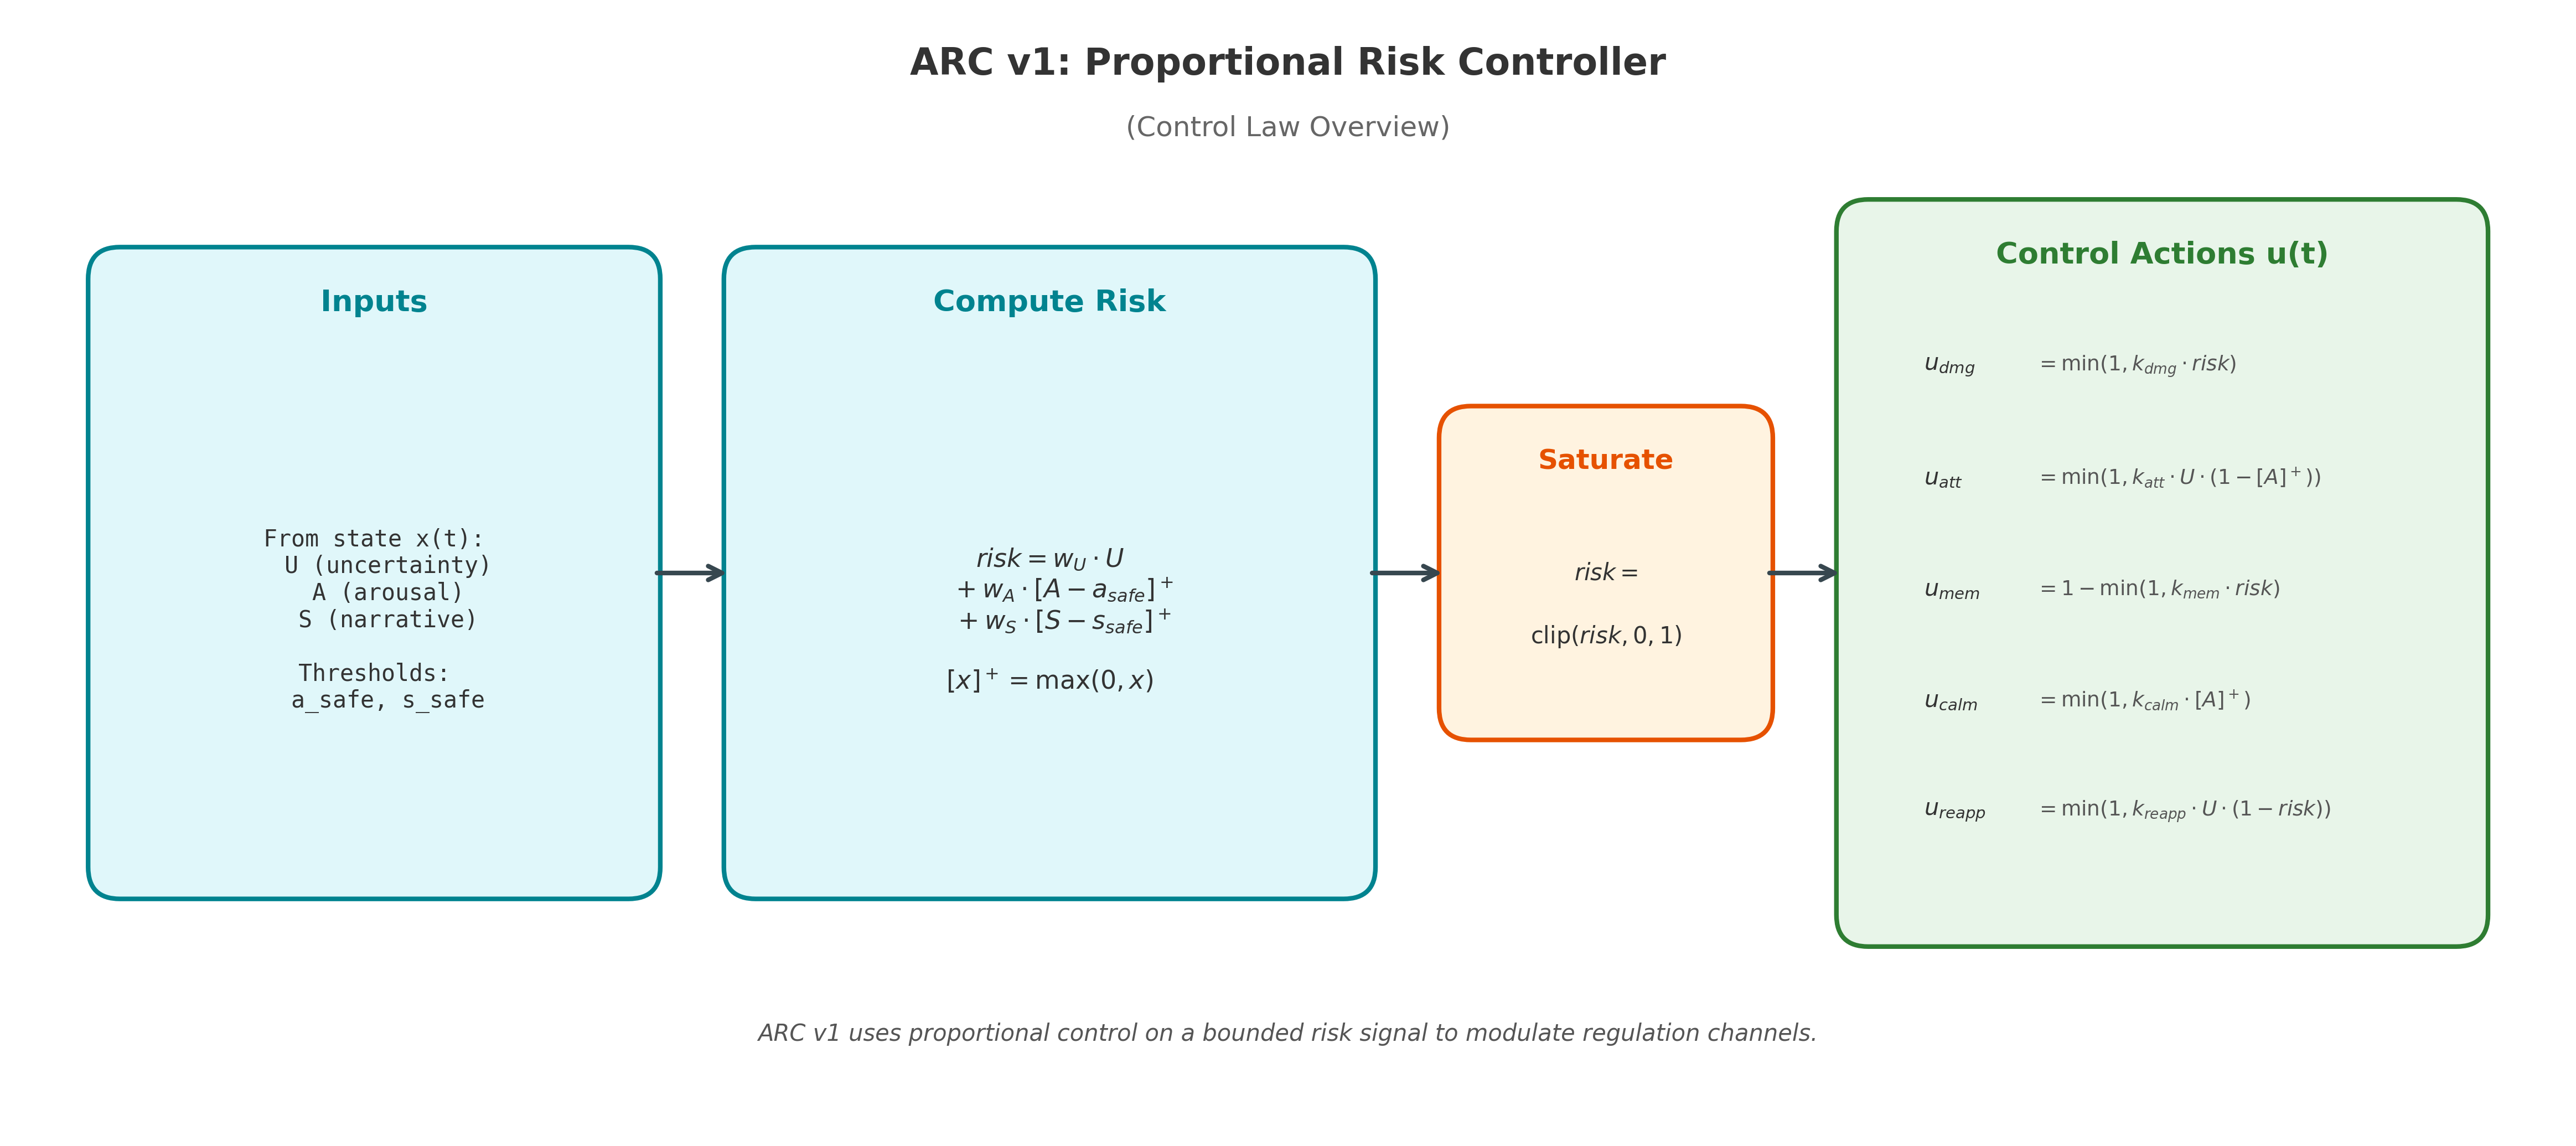
\includegraphics[width=0.8\textwidth]{figures/fig_arc_v1_controller.png}
    \caption{Resumen de la ley de control de ARC v1. Una señal de riesgo acotada impulsa un conjunto de acciones de regulación saturadas (supresión DMN, impulso de atención, memory gating, calma y reinterpretación).}
    \label{fig:arc_v1}
\end{figure}

\subsubsection{Controladores PID}

\textbf{ARC v1 PID:} Agrega términos integral y derivativo:
\begin{equation}
u(t) = K_p \cdot e(t) + K_i \cdot \int e(\tau) d\tau + K_d \cdot \frac{de}{dt}
\end{equation}
El término integral sobre el error narrativo ($S$) elimina la rumiación en estado estacionario (RI $\to$ 0).

\subsubsection{Controladores Óptimos (LQR/LQI)}

\textbf{ARC v1 LQR:} Regulador Lineal-Cuadrático con ganancias de la ecuación de Riccati:
\begin{equation}
K^* = (R + B^T P B)^{-1} B^T P A
\end{equation}
donde $P$ resuelve la Ecuación Algebraica de Riccati Discreta (DARE).

\textbf{ARC v1 LQI:} LQR + aumento integral para error estacionario cero.

\subsubsection{Controladores Jerárquicos}

\textbf{ARC v2 Jerárquico:} Control multi-escala temporal:
\begin{itemize}
    \item \textbf{Bucle rápido} (cada paso): regulación de arousal
    \item \textbf{Bucle medio} (cada 5 pasos): supresión narrativa
    \item \textbf{Bucle lento} (cada 20 pasos): adaptación del setpoint
\end{itemize}

\textbf{ARC v2 LQI:} Estructura jerárquica + LQI para anti-rumiación.

\subsubsection{Controladores Adaptativos}

\textbf{ARC v3 Meta-Control:} Programación de ganancias basada en el historial de desempeño:
\begin{equation}
K(t) = K_{base} \cdot f(\bar{P}_{20})
\end{equation}
donde $\bar{P}_{20}$ es el desempeño promedio móvil de 20 pasos.

\textbf{ARC Adaptive:} Optimización de parámetros en línea usando adaptación libre de gradiente.

\subsubsection{Controladores Robustos y Predictivos}

\textbf{ARC Robust (robusto-por-destemplado, motivado por $H_\infty$):} Ganancias conservadoras con márgenes de estabilidad diseñados para las peores perturbaciones. Enfatizamos que este controlador está \emph{motivado} por principios de diseño $H_\infty$ pero no es una síntesis $H_\infty$ completa: no resolvemos la DARE para transferencia de norma-$\ell_\infty$ mínima, y las ganancias se desafinan manualmente desde la solución LQR para proporcionar márgenes de estabilidad. Una variante ARC con síntesis $H_\infty$ real se lista como trabajo futuro.

\textbf{ARC Ultimate (MPC+LQI+Meta):} Control Predictivo Basado en Modelo con horizonte de 5 pasos, combinado con LQI y meta-control:
\begin{equation}
u(t) = \alpha \cdot u_{LQI}(t) + \beta \cdot u_{MPC}(t) \cdot \gamma_{meta}(t)
\end{equation}

\begin{table}[htbp]
\centering
\caption{Resumen de Arquitecturas de Controlador}
\label{tab:controllers}
\resizebox{\textwidth}{!}{%
\begin{tabular}{@{}lllll@{}}
\toprule
Controlador & Tipo & Anti-Rumiación & Óptimo & Adaptativo \\ \midrule
No Control (\texttt{no\_control}) & Baseline & No & No & No \\
Naive Calm (\texttt{naive\_calm}) & Baseline & No & No & No \\
Perf Optimized (\texttt{perf\_optimized}) & Baseline & No & No & No \\
ARC v1 (\texttt{arc\_v1}) & P & No & No & No \\
ARC v1 PID (\texttt{arc\_v1\_pid}) & PID & Sí (integral) & No & No \\
ARC v1 LQR (\texttt{arc\_v1\_lqr}) & LQR & No & Sí (Riccati) & No \\
ARC v1 LQI (\texttt{arc\_v1\_lqi}) & LQR+I & Sí (integral) & Sí & No \\
ARC v2 Hier (\texttt{arc\_v2\_hier}) & Multi-escala & No & No & No \\
ARC v2 LQI (\texttt{arc\_v2\_lqi}) & Multi+I & Sí (integral) & Sí & No \\
ARC v3 Meta (\texttt{arc\_v3\_meta}) & Adaptativo & No & No & Sí \\
ARC v3 PID Meta (\texttt{arc\_v3\_pid\_meta}) & PID+Meta & Sí (integral) & No & Sí \\
ARC v3 LQR Meta (\texttt{arc\_v3\_lqr\_meta}) & LQR+Meta & No & Sí & Sí \\
ARC Robust (\texttt{arc\_robust}) & H$\infty$ & Sí (robusto) & No & No \\
ARC Adaptive (\texttt{arc\_adaptive}) & Auto-ajuste & Sí (adaptativo) & No & Sí \\
ARC Ultimate (\texttt{arc\_ultimate}) & MPC+LQI+Meta & Sí & Sí & Sí \\ \bottomrule
\end{tabular}%
}
\end{table}

\subsection{ARC en el Bucle del Agente}

ARC se implementa como un wrapper ligero alrededor del paso/actualización de un agente. En cada instante, ARC lee el estado interno $\mathbf{x}(t)$ y las señales exógenas (recompensa, error de predicción, incertidumbre), calcula una señal de riesgo acotada, y aplica acciones de control que modulan la \textit{ganancia narrativa}, la \textit{atención}, la \textit{escritura en memoria} y el \textit{amortiguamiento del arousal}. La señal de control resultante puede usarse:
\begin{itemize}
    \item \textbf{Dentro de las dinámicas del estado} (Apéndices~B y~C), o
    \item \textbf{Dentro del bucle de aprendizaje}, p.\ ej., compuerta de actualizaciones de Q-learning bajo riesgo alto (Sección 6.7).
\end{itemize}

\textbf{Paso de ARC (conceptual):}
\begin{enumerate}
    \item Observar $(\mathbf{x}(t), PE(t), R(t), U_{\text{exog}}(t))$
    \item Calcular $\text{risk}(t)$
    \item Calcular $\mathbf{u}(t)$ con saturación a $[0,1]$
    \item Aplicar $\mathbf{u}(t)$ a las dinámicas de estado y/o a las actualizaciones de aprendizaje
\end{enumerate}

\begin{figure}[htbp]
    \centering
    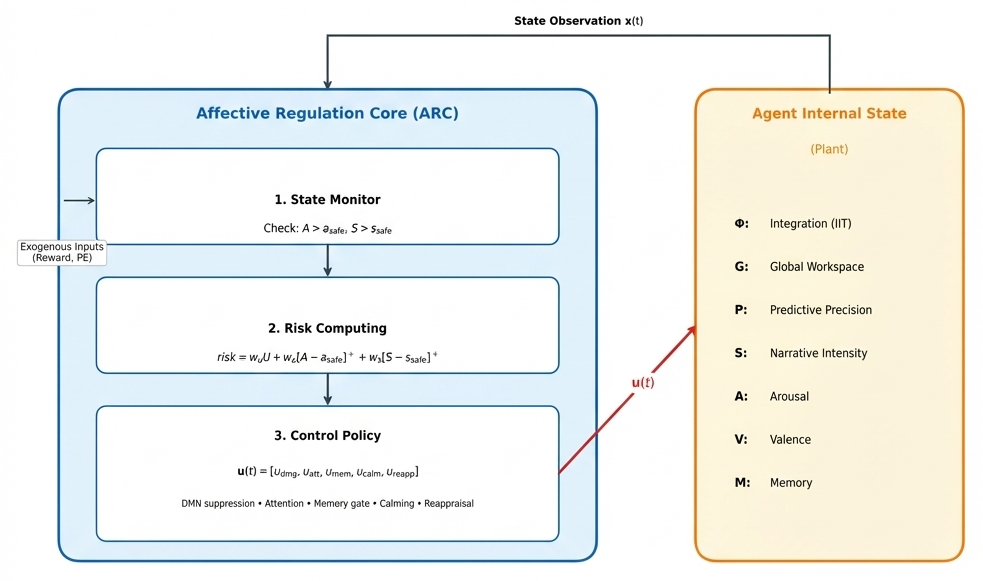
\includegraphics[width=\textwidth]{figures/fig_arc_architecture_v2_cropped.png}
    \caption{Arquitectura de ARC: el Núcleo de Regulación Afectiva actúa como un wrapper homeostático alrededor del agente, procesando el estado interno, las señales exógenas y aplicando acciones de control.}
    \label{fig:architecture}
\end{figure}

\subsection{Objetivo de Seguridad y Costo de Control}

ARC impone una \textit{región de operación segura} definida por los umbrales $(a_{safe}, s_{safe})$. Las desviaciones incrementan $\text{risk}(t)$ y disparan intervención proporcional. También medimos el \textbf{ControlEffort}, la magnitud promedio por paso de la intervención (Apéndice D), para capturar el costo/eficiencia de la regulación.

\subsection{Propiedades Teóricas}

Para formalizar las dinámicas de regulación enunciamos un lema elemental (la propiedad de rechazo de perturbación de la acción integral aplicada a nuestra abstracción escalar con fuga) y una observación que contextualiza un resultado estándar de control adaptativo. Deliberadamente no etiquetamos el enunciado de control adaptativo como una Proposición: es una cita directa de \cite{Astrom2008} especializada a nuestro controlador, no un resultado nuevo. Nuestra contribución consiste en contextualizar estos hechos para el entorno ASSB y vincularlos a los hallazgos empíricos (la falla por windup en L5, la deriva en escenarios benignos de \texttt{arc\_adaptive}), no en probar los resultados subyacentes de la teoría de control.

\paragraph{Lema 1 (La acción integral rechaza la presión constante de rumiación).}
Considere la dinámica simplificada (sin clipping) en tiempo discreto de la desviación narrativa
\[
\tilde{S}_{t+1} = (1-\mu)\tilde{S}_t + d - k\,u_t .
\]
donde $\tilde{S}_t = S_t - S_0$, $\mu\in(0,1)$ es un término de fuga, $k>0$ es una ganancia de control y $d$ es una perturbación constante desconocida (presión persistente de rumiación).

(i) Bajo control proporcional $u_t = K_p\tilde{S}_t$, el único equilibrio es $\tilde{S}_\infty = \dfrac{d}{\mu + kK_p}$, que es distinto de cero siempre que $d\neq 0$.

(ii) Bajo control PI con estado integral $z_{t+1}=z_t + \tilde{S}_t$ y ley de control $u_t = K_p\tilde{S}_t + K_i z_t$, cualquier equilibrio estable satisface necesariamente $\tilde{S}_\infty = 0$ (rechazo exacto del constante $d$), siempre que el equilibrio sea admisible (sin saturación).

\textit{Supuesto de estabilidad.} La afirmación (ii) presupone que la matriz de lazo cerrado
\[
A_{cl} = \begin{pmatrix} 1-\mu-kK_p & -kK_i \\ 1 & 1 \end{pmatrix}
\]
es Schur-estable (todos los eigenvalores estrictamente dentro del disco unitario). Esta condición define un conjunto abierto no vacío de ganancias admisibles $(K_p, K_i)$ para cualquier $\mu\in(0,1)$ y $k>0$, y se verifica fácilmente de forma numérica para las ganancias usadas en nuestros experimentos (Apéndice D).

\textit{Demostración:} Para (i), hacer $\tilde{S}_{t+1}=\tilde{S}_t=\tilde{S}_\infty$ y despejar. Para (ii), bajo el supuesto de Schur arriba, el estado aumentado $(\tilde{S}_t, z_t)$ converge a un punto fijo; en el equilibrio $z_{t+1}=z_t$ implica $\tilde{S}_\infty=0$, y sustituyendo en la actualización del estado se obtiene $0=d-k\,u_\infty$, de modo que el término integral aporta el desplazamiento constante necesario para cancelar $d$.

\textit{Observación:} Esta es una instancia en tiempo discreto del principio del modelo interno: rechazar perturbaciones constantes desconocidas requiere un integrador (o un observador de perturbaciones). Nótese que $RI$ puede ser cero aun si $\tilde{S}_\infty\neq 0$ siempre que $S_t \le s_{safe}$; la acción integral se requiere principalmente cuando se exige regulación estricta del setpoint y es vulnerable a windup bajo saturación (Sección 6.6).

\textit{Consecuencia crítica (teoría vs.\ empirismo).} La garantía del Lema~1 sólo es válida mientras la señal de control permanece en el interior del conjunto admisible $[0,1]$. Bajo acoplamiento adversarial (Sección~6.6, L5), el integrador satura y la garantía del modelo interno se rompe --- ésta es precisamente la falla por windup que observamos empíricamente para \texttt{arc\_lqi} y \texttt{arc\_pid}, y la motivación para los aumentos anti-windup discutidos en la Sección~7.5. En otras palabras, el Lema~1 caracteriza el régimen en el que la acción integral es provablemente beneficiosa; nuestro estudio empírico caracteriza el régimen en el que no lo es, y por qué se requieren extensiones robustas/jerárquicas.

\paragraph{Observación (requisito de persistencia de excitación para la variante adaptativa).}
Los resultados estándar en control adaptativo (\cite{Astrom2008}, Cap.~2--3) requieren \textit{persistencia de excitación} para la convergencia confiable de parámetros: si el vector de regresores no es suficientemente rico a lo largo de la trayectoria, el estimador de parámetros $\hat{\theta}$ puede derivar indefinidamente aun cuando el parámetro verdadero es constante. Aplicado al controlador \texttt{arc\_adaptive}, esto predice un desempeño pobre en escenarios benignos (baja varianza en las señales de recompensa / error de predicción que alimentan al estimador) seguido de una respuesta subóptima ante un shock repentino, porque la estimación no ha convergido cuando la perturbación llega. Esta es una cita de un resultado bien conocido, no una contribución: la enunciamos aquí sólo porque explica el patrón empírico específico observado para \texttt{arc\_adaptive} en las configuraciones baseline L1--L3 (Sección~7.3, ``Paradoja de la Adaptación''). No constituye una proposición original de este artículo.

\section{Benchmark ASSB}

\subsection{Escenarios}

ASSB está organizado como líneas de investigación (L1--L5 en simulación, L6 en RL). La suite completa de escenarios está implementada en \texttt{tasks/scenarios.py}.

\begin{figure}[htbp]
    \centering
    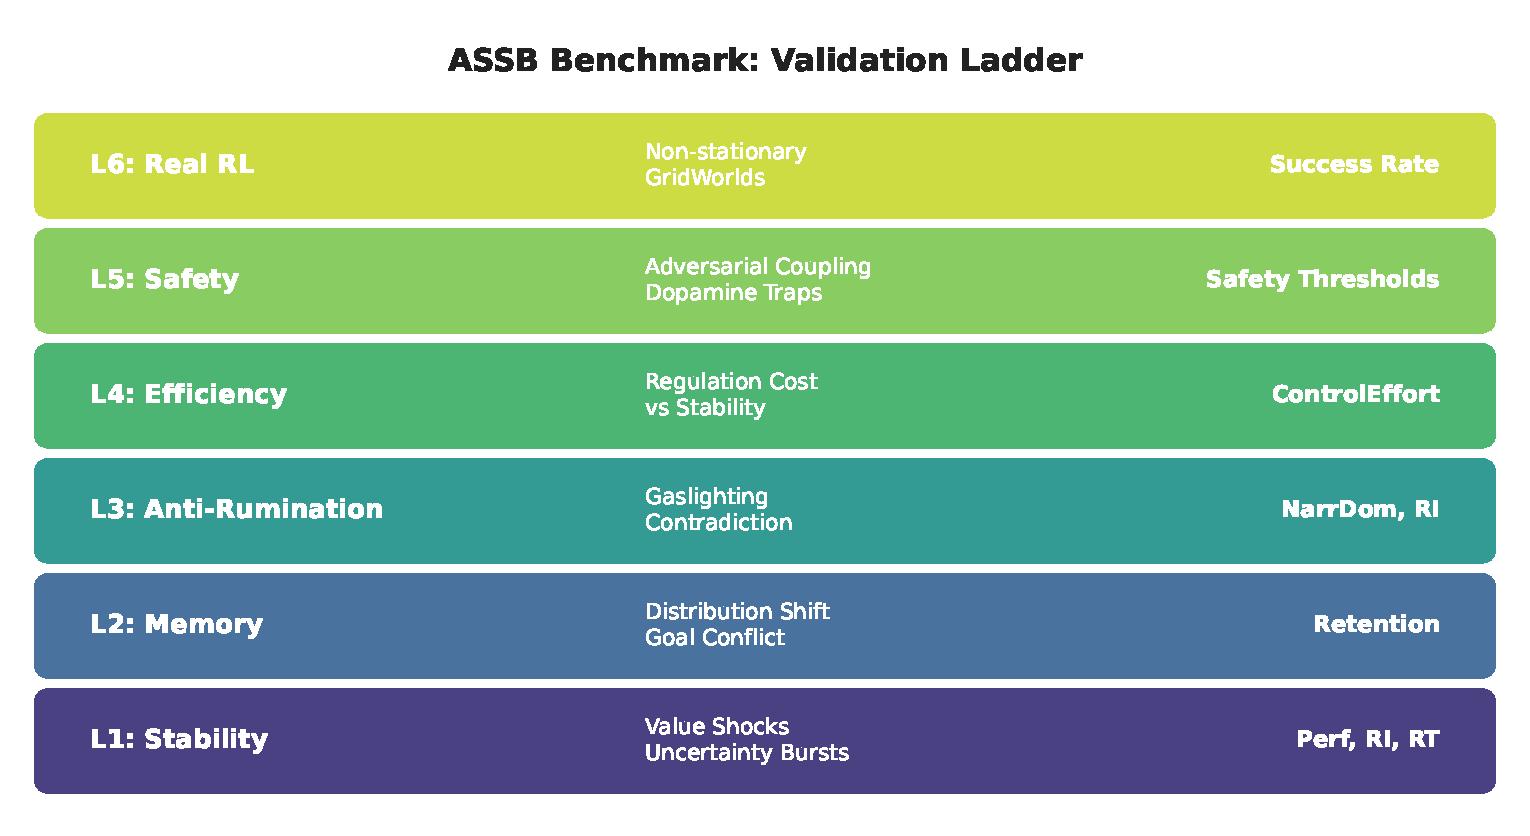
\includegraphics[width=\textwidth]{figures/fig_benchmark_ladder.pdf}
    \caption{Escalera de Validación ASSB: progresión desde pruebas de estabilidad (L1) hasta integración real con RL (L6).}
    \label{fig:ladder}
\end{figure}

\textit{Nota: L4 (Eficiencia de Control) se evalúa como análisis transversal sobre los escenarios L1--L3 en lugar de un escenario de perturbación dedicado.}

\subsection{Métricas}

\begin{itemize}
    \item \textbf{PerfMean}: desempeño promedio a lo largo del episodio (mayor = mejor; fórmula en Eq.~\ref{eq:perf}).
    \item \textbf{RT}: tiempo de recuperación post-shock, es decir el número de pasos tras el inicio de la perturbación $t_{\text{shock}}$ requeridos para que PerfMean regrese dentro del 10\% de su valor base previo al shock (menor = mejor; limitado en \texttt{rt\_max} cuando el criterio no se cumple; Apéndice D.2).
    \item \textbf{RI}: Índice de Rumiación, definido como la media de $[S_t - s_{\text{rum}\tau}]^{+}$ sobre el 80\% final del horizonte, es decir el exceso narrativo estacionario sobre el umbral de rumiación (menor = mejor; Apéndice D.4).
    \item \textbf{NDR}: Ratio de Dominancia Narrativa, es decir la fracción de pasos en los que la intensidad narrativa $S_t$ excede tanto el umbral seguro $s_{\text{safe}}$ como la salida de capacidad cognitiva $C_{\text{cog}}(t)$, indicando que el proxy de la Red Neuronal por Defecto está dominando el procesamiento orientado a meta (menor = mejor; Apéndice D.6).
    \item \textbf{ControlEffort}: magnitud $\ell_1$ promedio de la acción de control $\mathbf{u}(t)$ por paso (menor = más eficiente; Apéndice D.5).
\end{itemize}

Para los escenarios de aprendizaje continuo L2, reportamos además \textbf{Retention} (Apéndice D.7).

Las definiciones de métricas y sus implementaciones de referencia están en el Apéndice D y \texttt{metrics/metrics.py}.

\subsection{Líneas de Investigación: Justificación e Hipótesis}

ASSB está diseñado como una \textit{escalera de validación}: cada línea de investigación aumenta el realismo y los grados de libertad mientras pone a prueba un modo de falla distinto que aparece cuando los agentes portan estado interno tipo-afecto. El objetivo no es ``ganar'' un benchmark único, sino establecer si un mecanismo de regulación es (i) estable bajo shocks, (ii) preserva aprendizaje y memoria, (iii) resiste dinámicas de perseveración/manipulación, (iv) permanece eficiente y (v) transfiere a aprendizaje por refuerzo estándar.

Planteamos L1--L6 como hipótesis testables sobre \textit{qué componente es necesario} y \textit{qué métrica debería cambiar} si la regulación funciona:

\begin{itemize}
    \item \textbf{H1 (L1, estabilidad):} bajo shocks de valor/incertidumbre, los agentes regulados mantienen alto \textbf{PerfMean} mientras llevan \textbf{RI $\to$ 0} y reducen \textbf{RT} respecto a los baselines.
    \item \textbf{H2 (L2, memoria):} bajo cambio de distribución y conflicto de metas, el memory gating mejora \textbf{Retention} sin inducir rumiación (\textbf{RI}, \textbf{NDR}).
    \item \textbf{H3 (L3, anti-rumiación):} bajo entradas de tipo contradicción/manipulación, la supresión narrativa reduce \textbf{NDR} y \textbf{RI}, previniendo bucles de dominancia.
    \item \textbf{H4 (L4, eficiencia):} el meta-control reduce \textbf{ControlEffort} mientras mantiene desempeño/estabilidad (una mejora de Pareto vs.\ control de ganancia fija).
    \item \textbf{H5 (L5, seguridad adversarial):} cuando el entorno incentiva arousal alto o trampas dopaminérgicas, la regulación mantiene bajo \textbf{RI/NDR} sin colapso catastrófico del desempeño.
    \item \textbf{H6 (L6, RL real):} el aprendizaje tabular modulado por ARC se asocia con mayor tasa de éxito en transferencia no-estacionaria (métrica primaria L6: tasa de éxito; Tabla~\ref{tab:l6_results}). Las dinámicas afectivas internas en L6 no se miden a nivel de métricas ASSB (RI / NDR se definen sobre el espacio de estados simulado y no se calculan directamente para el wrapper de GridWorld); por lo tanto ``dinámicas afectivas acotadas'' es una propiedad de diseño del wrapper (por construcción, las señales de arousal/narrativa que expone están acotadas a $[0,1]$) más que un resultado probado independientemente. H6 se reporta como evidencia direccional, no como un efecto paramétricamente testeado.
\end{itemize}

\begin{table}[htbp]
\centering
\caption{Líneas de Investigación, Modos de Falla e Hipótesis}
\label{tab:hypotheses}
\resizebox{\textwidth}{!}{%
\begin{tabular}{@{}lllll@{}}
\toprule
Línea & Qué prueba & Modo de falla típico & Escenarios/entornos & Métricas primarias \\ \midrule
L1 & Estabilidad + recuperación bajo perturbación & Colapso post-shock; no-recuperación & \texttt{reward\_flip}, \texttt{noise\_burst}, \texttt{sudden\_threat} & PerfMean, RT, RI \\
L2 & Robustez de memoria (aprendizaje continuo) & Olvido catastrófico; sobreescritura por estrés & \texttt{distribution\_shift}, \texttt{goal\_conflict} & Retention, PerfMean, RI \\
L3 & Anti-rumiación bajo entradas tipo-manipulación & Bucles de dominancia narrativa & \texttt{sustained\_contradiction}, \texttt{gaslighting} & RI, NDR, PerfMean \\
L4 & Eficiencia de control & Sobrecontrol / intervención desperdiciada & ARC v3 meta vs ARC v1 & ControlEffort, PerfMean, RI \\
L5 & Seguridad bajo incentivos adversariales & Corrupción de metas; dinámicas buscadoras de arousal & \texttt{adversarial\_coupling}, \texttt{random\_dopamine} & RI, NDR, PerfMean \\
L6 & Integración con RL & Inestabilidad en el aprendizaje; mala transferencia & Variantes de GridWorld & Éxito, recompensa, estabilidad \\ \bottomrule
\end{tabular}%
}
\end{table}

Consideramos cada hipótesis soportada cuando sus métricas primarias se mueven en la dirección predicha respecto a los baselines y permanecen consistentes entre semillas (y entre escenarios donde aplique). La fuerza del soporte difiere por línea: H1--H3 se apoyan en contrastes ARC-vs-baseline donde la métrica primaria (PerfMean; RI en L1) se testa paramétricamente (Welch t-test, Sección~\ref{sec:statistical_analysis}); H4 (eficiencia de meta-control) y H6 (RL tabular) se reportan como soporte \emph{direccional} basado en estimaciones puntuales sobre 20 semillas, no como tests paramétricos de hipótesis (véase Sección~\ref{sec:statistical_analysis}, ``Alcance del testing paramétrico''). La distinción es explícita en la Sección~6 y la Tabla~\ref{tab:significance}.

\section{Experimentos}

\subsection{Protocolo Experimental y Baselines}

Validamos las hipótesis H1--H6 (Sección 5.3) corriendo las líneas de investigación correspondientes y evaluando las métricas primarias en la Tabla~\ref{tab:hypotheses}. Una hipótesis se trata como soportada cuando sus métricas primarias cambian en la dirección predicha respecto a los baselines, consistentemente entre semillas; para H1--H3 este soporte se respalda con tests paramétricos de significancia sobre los contrastes principales PerfMean/RI (Sección~\ref{sec:statistical_analysis}), mientras que para H4 (meta-control) y H6 (RL tabular) el soporte es direccional (estimaciones puntuales sobre 20 semillas, sin test paramétrico reportado; véase Sección~\ref{sec:statistical_analysis}, ``Alcance del testing paramétrico'').

\textbf{Simulación (L1--L5).} Usamos \texttt{configs/v2.yaml} con horizonte $H=160$, inicio de perturbación $\text{shock}_t=60$ y 20 semillas aleatorias. Las tablas reportan métricas promedio entre semillas (y, cuando se agregan, entre escenarios). Recovery Time (RT) se satura en \texttt{rt\_max} cuando el criterio estricto de recuperación no se cumple (Apéndice D.2).

\textbf{Controladores (simulación).} Implementados en \texttt{controllers/controllers.py}:
\begin{itemize}
    \item \texttt{no\_control}: sin regulación ($\mathbf{u}=0$; compuerta de memoria abierta)
    \item \texttt{naive\_calm}: amortiguamiento sólo de arousal ($u_{calm}$ proporcional a $A-a_{safe}$)
    \item \texttt{perf\_optimized}: un baseline competitivo que impulsa la atención ($u_{att}$ constante) pero no regula afecto/narrativa
    \item \texttt{arc\_v1}: controlador proporcional de riesgo (ARC v1)
    \item \texttt{arc\_v2\_hier}, \texttt{arc\_v3\_meta}: variantes jerárquica y de meta-control usadas donde se indica
\end{itemize}

\textbf{Aprendizaje por refuerzo (L6).} Integramos ARC con Q-learning tabular \cite{Watkins1992, Sutton2018} en tres variantes de GridWorld. Las tasas de éxito se calculan sobre el último 20\% de los episodios de entrenamiento (véase \texttt{outputs\_L6\_robust/final\_metrics.csv}).

\subsection{L1: Estabilidad Bajo Perturbación (Simulación)}

\textbf{Hipótesis (H1):} Bajo shocks de valor/incertidumbre, los agentes regulados mantienen alto \textbf{PerfMean} mientras llevan \textbf{RI $\to$ 0} y reducen \textbf{RT} respecto a los baselines.

\textbf{Setup:} 20 semillas $\times$ 3 escenarios $\times$ 4 controladores (\texttt{reward\_flip}, \texttt{noise\_burst}, \texttt{sudden\_threat})

\textbf{Resultados (L1):} como se muestra en la Tabla \ref{tab:l1_results}:

\begin{table}[htbp]
\centering
\caption{Resultados de Estabilidad L1 (media sobre 3 escenarios L1 $\times$ 20 semillas). Los valores de RT son medias sobre el triplete de escenarios e incluyen, para cualquier semilla/escenario donde el criterio estricto de recuperación no se cumple dentro de la ventana de evaluación, una censura por la derecha en $\texttt{rt\_max}=100$ (Apéndice~D.2); por lo tanto RT $=100.0$ en una fila significa ``sin recuperación bajo el criterio estricto para ningún escenario/semilla L1'', no una recuperación literal de $100$ pasos. Para ARC, la celda RT $=45.2$ está dominada por la recuperación rápida en \texttt{reward\_flip} y \texttt{noise\_burst}, con censura sólo en \texttt{sudden\_threat}; los desgloses por-escenario están en el Apéndice~G.1.}
\label{tab:l1_results}
\begin{tabular}{@{}lccc@{}}
\toprule
Controlador & PerfMean & RI & RT \\ \midrule
arc\_v1 & \textbf{0.966} & \textbf{0.00} & 45.2 \\
no\_control & 0.297 & 1.41 & 100.0 \\
naive\_calm & 0.375 & 1.41 & 66.7 \\
perf\_optimized & 0.862 & 1.39 & 100.0 \\ \bottomrule
\end{tabular}
\end{table}

\textbf{Hallazgo clave:} En los escenarios de estabilidad L1, ARC v1 elimina la rumiación (RI=0.00) mientras alcanza un desempeño promedio de \textbf{96.6\%} (PerfMean = 0.966), comparado con 29.7\% para los agentes no controlados. Nótese que RI=0 aplica para ARC v1 específicamente en L1; a lo largo de todos los escenarios (L1--L5), el controlador proporcional exhibe RI=0.15 agregado (Tabla~\ref{tab:controller_comparison}), mientras los controladores con acción integral mantienen RI=0 globalmente. RT depende del escenario: ARC se recupera rápidamente en \texttt{reward\_flip}, más lentamente en \texttt{noise\_burst}, y no regresa completamente al baseline pre-shock en \texttt{sudden\_threat} bajo la definición estricta de RT (Apéndice D.2), a pesar de mantener alto PerfMean. Los valores agregados de RT para \texttt{no\_control} y \texttt{perf\_optimized} (ambos 100.0 en la Tabla~\ref{tab:l1_results}) reflejan de manera similar este criterio estricto: cuando la trayectoria nunca re-entra a la banda pre-shock dentro del horizonte del episodio, RT se satura en \texttt{rt\_max} independientemente del controlador --- así que la fila RT=100 indica ``no se detectó recuperación bajo el criterio estricto'' en lugar de un artefacto de saturación de la métrica específico de ARC.

\begin{figure}[htbp]
    \centering
    
\includegraphics[width=0.8\textwidth]{figures/ablation_summary.png}
    \caption{Resumen de ablación (\texttt{reward\_flip}, L1): eliminar la supresión DMN (\texttt{u\_dmg}) causa rumiación y no-recuperación, indicando que el control DMN es necesario para la estabilidad bajo shocks de valor.}
    \label{fig:ablation}
\end{figure}

\subsection{L2: Memoria y Aprendizaje Continuo (Simulación)}

\textbf{Hipótesis (H2):} Bajo cambio de distribución y conflicto de metas, el memory gating mejora \textbf{Retention} sin inducir rumiación (\textbf{RI}, \textbf{NDR}).

\textbf{Setup:} 20 semillas $\times$ 2 escenarios (\texttt{distribution\_shift}, \texttt{goal\_conflict}) $\times$ 4 controladores

\textbf{Resultados (distribution\_shift):} los resultados se resumen en la Tabla \ref{tab:l2_results}:

\begin{table}[htbp]
\centering
\caption{Resultados de Memoria L2 (distribution\_shift)}
\label{tab:l2_results}
\begin{tabular}{@{}lccc@{}}
\toprule
Controlador & PerfMean & Retention & RI \\ \midrule
arc\_v1 & \textbf{0.972} & \textbf{1.00} & \textbf{0.00} \\
no\_control & 0.199 & 0.00 & 1.41 \\
naive\_calm & 0.276 & 0.15 & 1.41 \\
perf\_optimized & 0.869 & 0.94 & 1.39 \\ \bottomrule
\end{tabular}
\end{table}

\textbf{Hallazgo clave:} ARC mantiene una retención casi perfecta tras un cambio de distribución mientras mantiene la rumiación en cero; los baselines o bien olvidan (baja retención) o retienen con rumiación severa.

\subsection{L3: Pruebas de Estrés Anti-Rumiación (Simulación)}

\textbf{Hipótesis (H3):} Bajo entradas de tipo contradicción/manipulación, la supresión narrativa reduce \textbf{NDR} y \textbf{RI}, previniendo bucles de dominancia.

\textbf{Setup:} 20 semillas $\times$ 3 escenarios (\texttt{sustained\_contradiction}, \texttt{gaslighting}, \texttt{instruction\_conflict}) $\times$ 4 controladores (véase Tabla \ref{tab:l3_results}).

\begin{table}[htbp]
\centering
\caption{Resultados Anti-Rumiación L3}
\label{tab:l3_results}
\begin{tabular}{@{}lcccc@{}}
\toprule
Escenario & Controlador & PerfMean & RI & NDR \\ \midrule
sustained\_cont & arc\_v1 & \textbf{0.817} & \textbf{0.00} & \textbf{0.00} \\
sustained\_cont & no\_control & 0.014 & 1.47 & 0.99 \\
gaslighting & arc\_v1 & \textbf{0.980} & \textbf{0.00} & \textbf{0.00} \\
gaslighting & no\_control & 0.171 & 1.43 & 0.88 \\
instruction\_conf & arc\_v1 & \textbf{0.826} & 0.36 & \textbf{0.00} \\
instruction\_conf & no\_control & 0.034 & 1.45 & 0.97 \\ \bottomrule
\end{tabular}
\end{table}

\textbf{Hallazgo clave:} Bajo contradicción sostenida y entradas tipo-manipulación, los agentes no controlados entran en bucles de rumiación de alto NDR; ARC mantiene la dominancia narrativa cerca de cero y preserva el desempeño.

\subsection{L4: Eficiencia del Meta-Control}

\textbf{Hipótesis (H4):} El meta-control reduce \textbf{ControlEffort} mientras mantiene desempeño/estabilidad (una mejora de Pareto vs.\ control de ganancia fija).

\textbf{Setup:} ARC v3 (programación de ganancias) vs ARC v1 (véase Tabla \ref{tab:l4_results}).

\begin{table}[htbp]
\centering
\caption{Eficiencia del Meta-Control L4 (agregada)}
\label{tab:l4_results}
\begin{tabular}{@{}lccc@{}}
\toprule

Controlador & PerfMean & RI & ControlEffort \\ \midrule
arc\_v3\_meta & \textbf{0.941} & 0.090 & \textbf{0.615} \\
arc\_v1 & 0.934 & 0.148 & 0.777 \\ \bottomrule
\end{tabular}
\end{table}

\textbf{Hallazgo clave:} El meta-control reduce el esfuerzo de control en un \textbf{20.9\%} (de 0.777 a 0.615 en el agregado de 10 escenarios) mientras mejora ligeramente el desempeño agregado ($+0.7\%$). El RI agregado baja de 0.148 a 0.090 ($-39\%$ relativo), pero esta cifra debe leerse con cuidado: ambos agregados incluyen escenarios (L1 \texttt{reward\_flip}, \texttt{noise\_burst}) donde ambos controladores ya tienen RI $=0$ y por lo tanto contribuyen cero a la diferencia; la reducción se concentra en los escenarios más difíciles (\texttt{random\_dopamine}: $1.12 \rightarrow 0.26$; \texttt{instruction\_conflict}: $0.36 \rightarrow 0.25$, por Tablas~\ref{tab:g8_instruction_conflict} y~\ref{tab:g11_random_dopamine}), de modo que ``$-39\%$ agregado'' es una media-de-medias que mezcla celdas de diferencia-cero con celdas de diferencia-grande. Los desgloses por-escenario están en el Apéndice~G; un resumen no paramétrico (mediana de ratios por-escenario) queda como trabajo futuro.

\subsection{L5: Seguridad Bajo Condiciones Adversariales (Simulación)}

\textbf{Hipótesis (H5):} Cuando el entorno incentiva arousal alto o trampas dopaminérgicas, la regulación mantiene bajo \textbf{RI/NDR} sin colapso catastrófico del desempeño.

\textbf{Setup:} Entornos adversariales (\texttt{adversarial\_coupling}, \texttt{random\_dopamine}), 20 semillas (resultados en Tabla \ref{tab:l5_results}).

\begin{table}[htbp]
\centering
\caption{Resultados de Seguridad Adversarial L5 (controladores seleccionados incluyendo casos de falla)}
\label{tab:l5_results}
\begin{tabular}{@{}lcccc@{}}
\toprule
Escenario & Controlador & PerfMean & RI & NDR \\ \midrule
adversarial\_coupling & arc\_v1 & \textbf{0.963} & \textbf{0.00} & \textbf{0.00} \\
adversarial\_coupling & arc\_v3\_meta & 0.914 & 0.16 & 0.00 \\
adversarial\_coupling & no\_control & 0.409 & 1.47 & 0.96 \\
adversarial\_coupling & arc\_v1\_pid$^\dagger$ & 0.139 & 0.00 & 0.00 \\
adversarial\_coupling & arc\_v1\_lqi$^\dagger$ & 0.139 & 0.01 & 0.00 \\
adversarial\_coupling & arc\_ultimate$^\dagger$ & 0.134 & 0.01 & 0.00 \\
\midrule
random\_dopamine & arc\_v3\_meta & \textbf{0.905} & 0.26 & \textbf{0.00} \\
random\_dopamine & arc\_v1 & 0.897 & 1.12 & 0.58 \\
random\_dopamine & no\_control & 0.040 & 1.46 & 0.95 \\ \bottomrule
\end{tabular}

\vspace{0.5em}
\footnotesize{$^\dagger$ Colapso del controlador integral: el desempeño cae \textit{por debajo} del baseline no controlado debido al windup del integrador (véase el texto).}
\end{table}

\textbf{Hallazgo clave:} ARC mantiene la estabilidad aun bajo ataque adversarial. Sin embargo, descubrimos un \textbf{modo de falla crítico}: los controladores con fuerte acción integral (PID, LQI, Ultimate) \textbf{colapsan} en \texttt{adversarial\_coupling} (desempeño $< 0.20$), desempeñándose peor que el agente no controlado (0.41). Esto ocurre porque el entorno premia el arousal alto, causando que el término integral acumule error indefinidamente (``windup integral'') y suprima excesivamente la actividad del agente. El desglose completo por-controlador se proporciona en el Apéndice G.5 (Tabla~\ref{tab:g10_adversarial_coupling}). Este hallazgo sugiere que para defensa adversarial, los controladores proporcionales o robustos son estrictamente superiores a los integrales, y que \textbf{H5 sólo se soporta parcialmente}: la regulación preserva la seguridad (bajo RI/NDR) para controladores no integrales, pero las variantes integrales exhiben colapso catastrófico del desempeño.

\subsection{L6: Validación con RL Real}

\textbf{Hipótesis (H6):} El aprendizaje tabular modulado por ARC se asocia con mayor tasa de éxito en transferencia no-estacionaria (métrica primaria L6: tasa de éxito; Tabla~\ref{tab:l6_results}). Las dinámicas afectivas internas en L6 no se miden a nivel de métricas ASSB (RI / NDR se definen sobre el espacio de estados simulado y no se calculan directamente para el wrapper de GridWorld); por lo tanto ``dinámicas afectivas acotadas'' es una propiedad de diseño del wrapper (por construcción, las señales de arousal/narrativa que expone están acotadas a $[0,1]$) más que un resultado probado independientemente. H6 se reporta como evidencia direccional, no como un efecto paramétricamente testeado.

\textbf{Setup:} Integración Q-Learning + ARC en entornos GridWorld, 20 semillas $\times$ 200 episodios (éxito calculado sobre el último 20\% de episodios; véase Tabla \ref{tab:l6_results} y \texttt{outputs\_L6\_robust/final\_metrics.csv}).

\begin{table}[htbp]
\centering
\caption{Resultados de Validación con RL L6 (Tasas de Éxito)}
\label{tab:l6_results}
\begin{tabular}{@{}lccc@{}}
\toprule
Entorno & Éxito Baseline & Éxito ARC & Mejora \\ \midrule
GridWorld & 100\% & 100\% & 0\% \\
StochasticGridWorld & 100\% & 100\% & 0\% \\
\textbf{ChangingGoalGridWorld} & 39.9\% & \textbf{59.8\%} & \textbf{+49.8\%} \\ \bottomrule
\end{tabular}
\end{table}

\textbf{Hallazgo clave:} En entornos no-estacionarios, el wrapper ARC-RL integrado mejora la tasa de éxito de transferencia en \texttt{ChangingGoalGridWorld} (39.9\% $\rightarrow$ 59.8\%, $+49.8\%$ relativo). Esta es una estimación puntual a partir de 20 semillas; no reportamos un test paramétrico de significancia para el bloque L6 (los otros dos entornos, \texttt{GridWorld} y \texttt{StochasticGridWorld}, están en el techo de 100\% tanto para el baseline como para ARC, de modo que una comparación a nivel de suite se reduce al único entorno no saturado, y presentamos el resultado como evidencia direccional más que como un efecto testeado por hipótesis). El estudio de ablación en \texttt{ChangingGoalGridWorld} aísla la contribución de cada mecanismo (Tabla \ref{tab:l6_ablation}). Los valores de ablación se calculan a partir de los mismos artefactos de corrida L6 (\texttt{outputs\_L6\_robust/summary.csv}, \texttt{outputs\_L6\_robust/raw\_results.csv}).

\begin{table}[htbp]
\centering
\footnotesize
\caption{Resultados de Ablación L6 (ChangingGoalGridWorld)}
\label{tab:l6_ablation}
\begin{tabular}{lrr}
    \toprule
    Configuración del agente & Tasa de Éxito & Recompensa Final (media) \\
    \midrule
    Q-Learning vainilla (Baseline) & 39.9\% & -0.40 \\
    ARC (sólo Memory Gating) & \textbf{71.8\%} & \textbf{0.24} \\
    ARC (sólo Detección de Cambio) & 65.6\% & 0.13 \\
    Wrapper ARC completo (ambos) & 59.8\% & -0.02 \\
    \bottomrule
\end{tabular}
\end{table}

Los resultados revelan que el \textbf{memory gating} por sí solo alcanza la tasa de éxito individual más alta (71.8\%), sugiriendo que proteger el conocimiento aprendido de la sobreescritura catastrófica es el factor dominante en tareas no-estacionarias. La \textbf{detección de cambio} por sí sola también supera al baseline (65.6\% vs.\ 39.9\%). Curiosamente, combinar ambos mecanismos (59.8\%) rinde peor que cualquiera de los componentes por separado. \emph{Hipotetizamos} una interacción sub-aditiva (la detección de cambio aumenta la exploración justo cuando el memory gating intenta proteger el conocimiento existente, creando presiones opuestas sobre la tasa de aprendizaje), pero enfatizamos que esta es una lectura mecanística post-hoc, no un resultado causal: una ablación de la composición temporal (p.\ ej., activar el memory gating sólo fuera de los shifts detectados) sería necesaria para aislar el efecto, y queda como trabajo futuro.

\paragraph{Resultado negativo: wrapper de plasticidad DQN (límite de alcance).}
Para probar la validez externa más allá del Q-learning tabular, corrimos una suite de 10 semillas de Deep RL usando Stable-Baselines3 DQN con un wrapper de plasticidad ARC que modula la tasa de aprendizaje, la exploración, el muestreo del replay y la compuerta de actualizaciones con base en las señales de regulación de ARC. Tanto en \texttt{NonStationaryCartPole} como en \texttt{CatastrophicForgettingEnv}, \textbf{la plasticidad ARC rindió por debajo del DQN baseline} en recompensa media y tasa de éxito (Apéndice~\ref{sec:dqn_suite}, Tabla~\ref{tab:g13_l6b_dqn}). La plasticidad ARC sí redujo la varianza de la recompensa (consistente con el efecto estabilizador observado en simulación), pero con un costo sustancial de desempeño que atribuimos a (i)~disrupción del flujo de gradiente por la compuerta de actualizaciones, (ii)~interferencia en la distribución del replay por el muestreo consciente del cambio, y (iii)~desajuste de hiperparámetros entre la calibración ASSB y la escala de recompensa de CartPole. Reportamos este hallazgo negativo de manera transparente y lo usamos para delimitar el límite de aplicabilidad actual de ARC: \emph{los mecanismos validados en L6 transfieren a RL tabular pero requieren rediseño arquitectónico para aprendices basados en gradiente} (Sección~\ref{sec:future_work}). Esto motiva alternativas de modulación suave (escalamiento de la tasa de aprendizaje, re-ponderación de la loss) y despliegues a nivel de agente donde el estado interno sea explícito en lugar de emergente (p.\ ej., agentes cognitivos basados en LLM \cite{Damian2026b}).

\begin{figure}[htbp]
    \centering
    
\includegraphics[width=\textwidth]{figures/learning_curves.png}
    \caption{Curvas de aprendizaje comparando Q-learning modulado por ARC (cian) vs.\ Q-learning baseline (naranja) en GridWorld, StochasticGridWorld y ChangingGoalGridWorld. Las bandas sombreadas muestran $\pm$1 std sobre 20 semillas.}
    \label{fig:learning_curves}
\end{figure}

\subsection{Análisis Estadístico}\label{sec:statistical_analysis}
Para asegurar rigor, realizamos un análisis estadístico exhaustivo sobre todos los experimentos.

\subsubsection{Tests de Significancia}
Condujimos tests de Welch de dos muestras independientes (asumiendo varianzas desiguales) comparando ARC vs.\ baseline (no\_control) para cada métrica y línea de investigación (Tabla \ref{tab:significance}). Dadas 5 comparaciones simultáneas, aplicamos la corrección de Bonferroni ($\alpha_{adj} = 0.05/5 = 0.01$); todos los p-valores reportados siguen siendo significativos bajo este umbral más estricto por varios órdenes de magnitud. Los tamaños de efecto se reportan como Cohen's d; los intervalos de confianza al 95\% basados en bootstrap no se inlinean en la Tabla~\ref{tab:significance} (los efectos son suficientemente grandes como para que los intervalos queden muy lejos de cruzar el cero, y los datos completos por-semilla se liberan en el paquete de reproducibilidad para lectores que deseen recalcularlos).

\textbf{Tamaño muestral.} Usamos 20 semillas por celda (controlador, escenario), seleccionadas para detectar Cohen's $d \geq 0.8$ (efecto ``grande'') con potencia estadística $\geq 0.95$ a $\alpha = 0.01$ bajo supuestos conservadores de varianza. Los tamaños de efecto observados post-hoc (Cohen's $d > 7$ para RI y PerfMean en L1--L3) exceden ampliamente este umbral, de modo que las conclusiones no están limitadas por potencia.

\textbf{Reporte de dispersión.} Para mantener las tablas del cuerpo compactas, reportamos medias por-celda; la dispersión dentro de cada grupo se resume con los Cohen's $d$ y p-valores en la Tabla~\ref{tab:significance} y se visualiza en los gráficos de comparación de controladores (Figura~\ref{fig:perf_rum}, Figura~\ref{fig:tradeoff_effort}). Los agregados a 3 decimales a nivel de escenario (que exponen implícitamente la varianza entre escenarios para cada controlador) se proporcionan en el Apéndice~G (Tablas~\ref{tab:g1_reward_flip}--\ref{tab:g11_random_dopamine}). Las salidas CSV por-semilla con std / IQR completos para cada celda (controlador, escenario, métrica) se liberan con el paquete de reproducibilidad; optamos por no inlinearlas en las tablas del cuerpo porque la grilla de 20 semillas $\times$ 15 controladores $\times$ 10 escenarios $\times$ 4 métricas comprometería la legibilidad.

\begin{table}[htbp]
\centering
\caption{Análisis de Significancia Estadística (ARC vs.\ Baseline)}
\label{tab:significance}
\begin{tabular}{@{}llccccc@{}}
\toprule
Línea & Métrica & Media ARC & Media Baseline & p-valor & Cohen's d & Sig. \\ \midrule
L1 & PerfMean & 0.966 & 0.297 & $2.84 \times 10^{-86}$ & 10.11 & *** \\
L1 & RI & 0.00 & 1.41 & ---$^\dagger$ & ---$^\dagger$ & ---$^\dagger$ \\
L2 & PerfMean & 0.972 & 0.283 & $9.78 \times 10^{-154}$ & 11.45 & *** \\
L3 & PerfMean & 0.935 & 0.204 & $2.77 \times 10^{-182}$ & 7.08 & *** \\
L5 & PerfMean & 0.943 & 0.208 & $< 10^{-200}$ & 8.41 & *** \\ \bottomrule
\end{tabular}
\end{table}

\textit{Todas las comparaciones reportadas numéricamente son estadísticamente significativas (p $<$ 0.001). Los valores de Cohen's d indican tamaños de efecto extremadamente grandes (d $>$ 0.8 se considera ``grande''). $^\dagger$Para la fila L1--RI deliberadamente no reportamos un p-valor paramétrico, Cohen's d ni marcador de significancia: el grupo ARC produce RI $= 0$ en las 20 semillas, de modo que la varianza intra-grupo es cero por construcción, y el test t de Welch no está bien planteado bajo esta condición (el estadístico de prueba diverge). En su lugar reportamos medidas de tamaño de efecto acotadas, libres de distribución, que sí están bien definidas: probabilidad de superioridad $\Pr(X_{\text{baseline}} > X_{\text{ARC}}) = 1.00$ y Cliff's $\delta = 1.00$, indicando separación completa (sin solapamiento) de las dos distribuciones. La conclusión sustantiva --- que los controladores ARC integrales llevan la rumiación a cero con varianza evanescente en estos escenarios --- se sostiene íntegramente con estas medidas libres de distribución y no depende de ningún test paramétrico.}

\textbf{Alcance del testing paramétrico.} La Tabla~\ref{tab:significance} reporta tests paramétricos (Welch) para el contraste principal de estabilidad/desempeño en L1--L3 y L5, es decir la comparación ARC vs.\ baseline en PerfMean (y RI en L1). \emph{No} reporta tests paramétricos para cada celda de cada métrica: no corremos tests de Welch sobre RT, NDR, Retention ni ControlEffort en el cuerpo, y explícitamente no corremos tests paramétricos sobre los bloques RL L6 / L6b (Sección~6.7, Apéndice~\ref{sec:dqn_suite}). Para esas métricas, nuestro reclamo no es ``diferencia estadísticamente significativa'' sino ``efecto direccional en la dirección hipotetizada, consistente con las medias y la dispersión visibles en las tablas del apéndice por-escenario y las medidas acotadas de tamaño de efecto sobre RI''. Cuando describimos H1--H6 como ``soportadas'' (Sección~5.3, Sección~6.9), la lectura pretendida es: las métricas primarias pre-registradas para cada línea se mueven en la dirección predicha; los tests paramétricos en la Tabla~\ref{tab:significance} cubren los contrastes principales PerfMean/RI; para métricas secundarias y para L6, el soporte es direccional, no formalmente testeado. Un análisis paramétrico completo por-métrica, por-escenario (con corrección por comparaciones múltiples) queda como trabajo futuro.

\subsubsection{Análisis de Correlación}
Analizamos las correlaciones entre métricas para entender la dinámica del sistema. La Tabla~\ref{tab:correlations} reporta tres pares pre-seleccionados por \emph{relevancia teórica} (cada uno evalúa una hipótesis específica de la Sección~5.3: PerfMean--RI aborda si la rumiación cuesta desempeño; RI--NDR valida cruzadamente dos medidas de bucle narrativo; RT--RI testea si recuperación lenta y rumiación co-ocurren). La matriz completa de correlaciones $11\times 11$ sobre todas las métricas ASSB está disponible en la Figura~\ref{fig:correlation_combined}, donde son visibles pares fuertes adicionales (p.\ ej., ControlEffort--PerfMean, Retention--PerfMean) y se discuten en el Apéndice~E pero no se resaltan aquí para evitar inflación por comparaciones múltiples.

\begin{table}[htbp]
\centering
\caption{Análisis de correlación resumido sobre todas las corridas experimentales}
\label{tab:correlations}
\begin{tabular}{@{}lcl@{}}
\toprule
Par de métricas & Correlación (r) & Interpretación \\ \midrule
PerfMean $\leftrightarrow$ RI & \textbf{-0.589} & Mayor rumiación tiende a reducir el desempeño \\
RI $\leftrightarrow$ NDR & \textbf{+0.92} & Rumiación y dominancia narrativa co-ocurren \\
RT $\leftrightarrow$ RI & \textbf{+0.44} & Recuperación más lenta correlaciona con rumiación \\ \bottomrule
\end{tabular}
\end{table}

\textbf{Insight clave:} A lo largo de controladores y escenarios, un Índice de Rumiación (RI) más alto tiende a reducir el desempeño medio. Sin embargo, algunos controladores óptimos (p.\ ej., LQR) pueden sostener PerfMean alto mientras exhiben RI alto, porque PerfMean incluye capacidad modulada por narrativa (Apéndice B). Esto motiva reportar RI como una métrica de seguridad separada.

\textbf{Advertencia sobre pooling (riesgo de paradoja de Simpson).} Las correlaciones anteriores se agrupan (pool) entre familias de controladores con comportamientos estructuralmente distintos. La familia LQR sostiene PerfMean alto con RI alto, mientras que los controladores con aumento integral llevan RI a cero independientemente de PerfMean; estas dos poblaciones empujan la pendiente pooled PerfMean--RI en direcciones opuestas, y el valor pooled $r=-0.589$ está más cerca de una media ponderada de pendientes intra-familia que de una descripción de cualquier familia individual. Por lo tanto reportamos las correlaciones pooled sólo como estadísticos de resumen; las correlaciones por-familia pueden diferir sustancialmente y, en principio, invertir el signo. Un análisis de correlación estratificado por familia de controlador queda como trabajo futuro; los lectores que deseen re-particionar pueden hacerlo directamente desde los CSVs por-semilla liberados con el paquete de reproducibilidad.

\subsubsection{Análisis de Robustez}
Finalmente, nuestras dinámicas de estado están diseñadas para plausibilidad funcional más que para fidelidad biológica, y el análisis formal de estabilidad (p.\ ej., pruebas de Lyapunov) queda como trabajo futuro. La validación actual se basa en el benchmarking empírico bajo un amplio rango de condiciones:
\begin{itemize}
    \item \textbf{Tendencia L1-L5:} las variantes ARC superan a los baselines en la mayoría de los entornos evaluados, con la excepción conocida bajo \texttt{adversarial\_coupling} donde los controladores integrales colapsan.
    \item \textbf{Varianza:} los controladores ARC generalmente exhiben menor varianza \emph{intra-escenario} (varianza entre semillas en un escenario fijo), indicando comportamiento más consistente a nivel de semilla. Esto \emph{no} se extiende a la varianza \emph{entre escenarios}: \texttt{arc\_adaptive}, por ejemplo, oscila de PerfMean $\approx 0.998$ en \texttt{reward\_flip} a $\approx 0.193$ en \texttt{adversarial\_coupling} --- un rango entre escenarios mayor que el de \texttt{no\_control}. El reclamo de ``menor varianza'' aquí se refiere sólo a la estrechez de los boxplots a nivel de semilla visible en la Figura~\ref{fig:perf_rum}, no a la robustez entre escenarios, que es el objeto del test de tres criterios en la Tabla~\ref{tab:three_criterion_test}.
    \item \textbf{Dificultad por escenario:} \texttt{sustained\_contradiction} es el más difícil (menor PerfMean de ARC: 0.817); \texttt{gaslighting} es el más fácil (0.980)
\end{itemize}

\begin{figure}[htbp]
    \centering
    
\includegraphics[width=0.8\textwidth]{figures/sensitivity_controller.png}
    \caption{Distribución de desempeño por tipo de controlador. Las variantes ARC (azul) superan consistentemente a los baselines (rojo) con menor varianza.}
    \label{fig:sensitivity}
\end{figure}

\subsection{Comparación de Arquitecturas de Controlador}

Más allá del controlador proporcional básico (ARC v1), implementamos y evaluamos múltiples arquitecturas de control inspiradas en teoría de control clásica y moderna. La Tabla~\ref{tab:controller_comparison} resume los resultados entre los 15 controladores (20 semillas $\times$ 10 escenarios; L1--L3, L5).

\begin{table}[htbp]
\centering
\caption{Comparación de Arquitecturas de Controlador (20 semillas $\times$ 10 escenarios L1--L3 / L5). Los valores están redondeados a 2 decimales para legibilidad; las cifras canónicas a 3 decimales de las que se derivan estas aparecen en la Tabla~\ref{tab:l4_results} (subconjunto L4 meta-control) y la Tabla~\ref{tab:g9_meta_control} (agregado), de modo que p.\ ej.\ \texttt{arc\_v1} RI $=0.15$ aquí corresponde a $0.148$ en la Tabla~\ref{tab:g9_meta_control}, y el esfuerzo de \texttt{arc\_v3\_meta} $=0.61$ aquí a $0.615$.}
\label{tab:controller_comparison}
\footnotesize
\begin{adjustbox}{max width=0.88\textwidth}
\begin{tabular}{@{}llcccc@{}}
\toprule
Controlador & Tipo & PerfMean & RI & Overshoot & ControlEffort \\ \midrule
no\_control & Baseline & 0.21 & 1.43 & 0.40 & 0.00 \\
naive\_calm & Baseline & 0.24 & 1.44 & 0.16 & 0.26 \\
perf\_optimized & Baseline & 0.85 & 1.43 & 0.40 & 0.70 \\
arc\_v1 & P & 0.93 & 0.15 & 0.29 & 0.78 \\
arc\_v1\_pid & PID & 0.87 & \textbf{0.00} & \textbf{0.00} & 2.40 \\
arc\_v1\_lqr & LQR & \textbf{0.96} & 1.42 & 0.14 & 0.88 \\
arc\_v1\_lqi & LQR+I & 0.88 & \textbf{0.00} & \textbf{0.00} & 1.14 \\
arc\_v2\_hier & Jerárquico & 0.93 & 1.22 & 0.29 & 0.65 \\
arc\_v2\_lqi & Jerár+LQI & 0.88 & \textbf{0.00} & \textbf{0.00} & 1.14 \\
arc\_v3\_meta & Meta & 0.94 & 0.09 & 0.17 & \textbf{0.61} \\
arc\_v3\_pid\_meta & PID+Meta & 0.91 & \textbf{0.00} & 0.24 & 1.57 \\
arc\_v3\_lqr\_meta & LQR+Meta & 0.84 & 1.44 & 0.32 & 0.94 \\
arc\_robust & H$\infty$ & \textbf{0.95} & \textbf{0.00} & 0.18 & 1.03 \\
arc\_adaptive & Adaptativo & 0.91 & \textbf{0.00} & \textbf{0.00} & 1.83 \\
arc\_ultimate & MPC+LQI & 0.89 & \textbf{0.00} & \textbf{0.01} & 1.33 \\ \bottomrule
\end{tabular}
\end{adjustbox}
\end{table}

\textbf{Hallazgos clave:}
\begin{enumerate}
    \item \textbf{LQR alcanza el mayor desempeño} (0.96) pero al costo de alta rumiación (RI $>$ 1.3), demostrando que optimizar ciegamente el estado matemático no elimina necesariamente los bucles patológicos.
    \item \textbf{Las variantes PID/LQI eliminan la rumiación} (RI=0) en entornos estocásticos pero \textbf{colapsan bajo acoplamiento adversarial} (PerfMean $< 0.14$; véase Sección 6.6 y Tabla~\ref{tab:g10_adversarial_coupling}), desempeñándose peor que el agente no controlado debido al windup integral.
    \item \textbf{El meta-control es el más eficiente entre las variantes ARC} (0.61 de esfuerzo) mientras mantiene alto desempeño. (Nota: \texttt{naive\_calm} tiene menor esfuerzo crudo en 0.26 pero alcanza sólo 0.24 de PerfMean, haciendo del meta-control el controlador \textit{efectivo} más eficiente.)
    \item \textbf{H$\infty$ Robust es la única variante ARC que pasa el test de consistencia de tres criterios} definido abajo (Tabla~\ref{tab:three_criterion_test}): alto desempeño en L1--L3, rumiación cero en L1--L5 \emph{incluyendo} acoplamiento adversarial, y ningún colapso por debajo del baseline no controlado en ningún escenario. Éste es el significado operacional de ``mejor balance global'' en el abstract.
    \item \textbf{Existe un trade-off} entre desempeño y anti-rumiación: los controladores integrales sacrifican $\sim$5\% de desempeño para eliminar los bucles perseverativos.
\end{enumerate}

\paragraph{Definición operacional de ``mejor balance global''.} En lugar de usar una escalarización ad-hoc, verificamos contra tres criterios falsables computados directamente desde la Tabla~\ref{tab:controller_comparison} y las tablas por-escenario del apéndice:
\begin{itemize}
    \item \textbf{C1 (alto desempeño):} PerfMean $\geq 0.93$ en cada escenario L1--L3 individualmente (no sólo en agregado).
    \item \textbf{C2 (cero rumiación):} RI $=0$ agregado sobre L1--L5, \emph{y} RI $=0$ específicamente en \texttt{adversarial\_coupling} (la prueba de estrés por windup).
    \item \textbf{C3 (sin colapso):} PerfMean por encima del baseline no controlado (PerfMean $=0.409$ en \texttt{adversarial\_coupling}, PerfMean $\approx 0.30$ en L1) en cada escenario.
\end{itemize}

Aplicando estos criterios a los 15 controladores de forma mecánica: C1 se chequea contra las tablas por-escenario L1--L3 (Tablas~\ref{tab:g1_reward_flip},~\ref{tab:g2_noise_burst},~\ref{tab:g3_sudden_threat} para L1; Tablas~\ref{tab:g4_distribution_shift},~\ref{tab:g5_goal_conflict} para L2; Tablas~\ref{tab:g6_sustained_contradiction},~\ref{tab:g7_gaslighting},~\ref{tab:g8_instruction_conflict} para L3), C2 contra la tabla L5 de acoplamiento adversarial (Tabla~\ref{tab:g10_adversarial_coupling}) y la columna RI agregada de la Tabla~\ref{tab:controller_comparison}, y C3 contra la Tabla~\ref{tab:g10_adversarial_coupling} (baseline PerfMean $=0.409$ en \texttt{adversarial\_coupling}) más las filas L1 de la Tabla~\ref{tab:l1_results}. El veredicto resultante es:

\begin{table}[H]
\centering
\footnotesize
\caption{Test de consistencia de tres criterios para controladores ARC. Sólo se listan como aprobados los controladores que pasan los tres criterios.}
\label{tab:three_criterion_test}
\begin{tabular}{@{}lccccc@{}}
\toprule
Controlador & Tipo & C1 & C2 & C3 & ¿Los tres? \\ \midrule
\texttt{arc\_robust}    & H$\infty$     & \checkmark & \checkmark & \checkmark & \textbf{Sí} \\
\texttt{arc\_v1}        & P             & \checkmark & $\times$    & \checkmark & No \\
\texttt{arc\_v1\_pid}   & PID           & $\times$    & \checkmark & $\times$    & No (windup) \\
\texttt{arc\_v1\_lqi}   & LQR+I         & $\times$    & \checkmark & $\times$    & No (windup) \\
\texttt{arc\_v2\_hier}  & Jerárquico    & \checkmark & $\times$    & \checkmark & No \\
\texttt{arc\_v3\_meta}  & Meta          & \checkmark & $\times$    & \checkmark & No \\
\texttt{arc\_v3\_pid\_meta} & PID+Meta  & $\times$    & \checkmark & \checkmark & No \\
\texttt{arc\_adaptive}  & Adaptativo    & \checkmark & \checkmark & $\times$    & No (colapsa en L5) \\
\texttt{arc\_ultimate}  & MPC+LQI       & $\times$    & \checkmark & $\times$    & No (windup) \\ \bottomrule
\end{tabular}
\end{table}
Sólo \texttt{arc\_robust} pasa los tres criterios simultáneamente, que es el sentido preciso en el que lo describimos como alcanzando el ``mejor balance global'' en el abstract. Nótese que \texttt{arc\_v3\_pid\_meta} falla C1 en \texttt{sustained\_contradiction} (PerfMean $=0.753 < 0.93$; véase Tabla~\ref{tab:g6_sustained_contradiction}); \texttt{arc\_adaptive} y todas las variantes sólo-integrales fallan C3 en \texttt{adversarial\_coupling}. Los criterios y su verificación son deliberadamente simples para que cualquier lector pueda re-chequearlos directamente desde las tablas.

Estos resultados sugieren que el despliegue práctico debería considerar el contexto de aplicación: los escenarios de alto riesgo pueden favorecer controladores robustos, mientras que los entornos con recursos limitados se benefician de la eficiencia del meta-control.

\subsubsection{Comparaciones Visuales}

\begin{figure}[htbp]
    \centering
    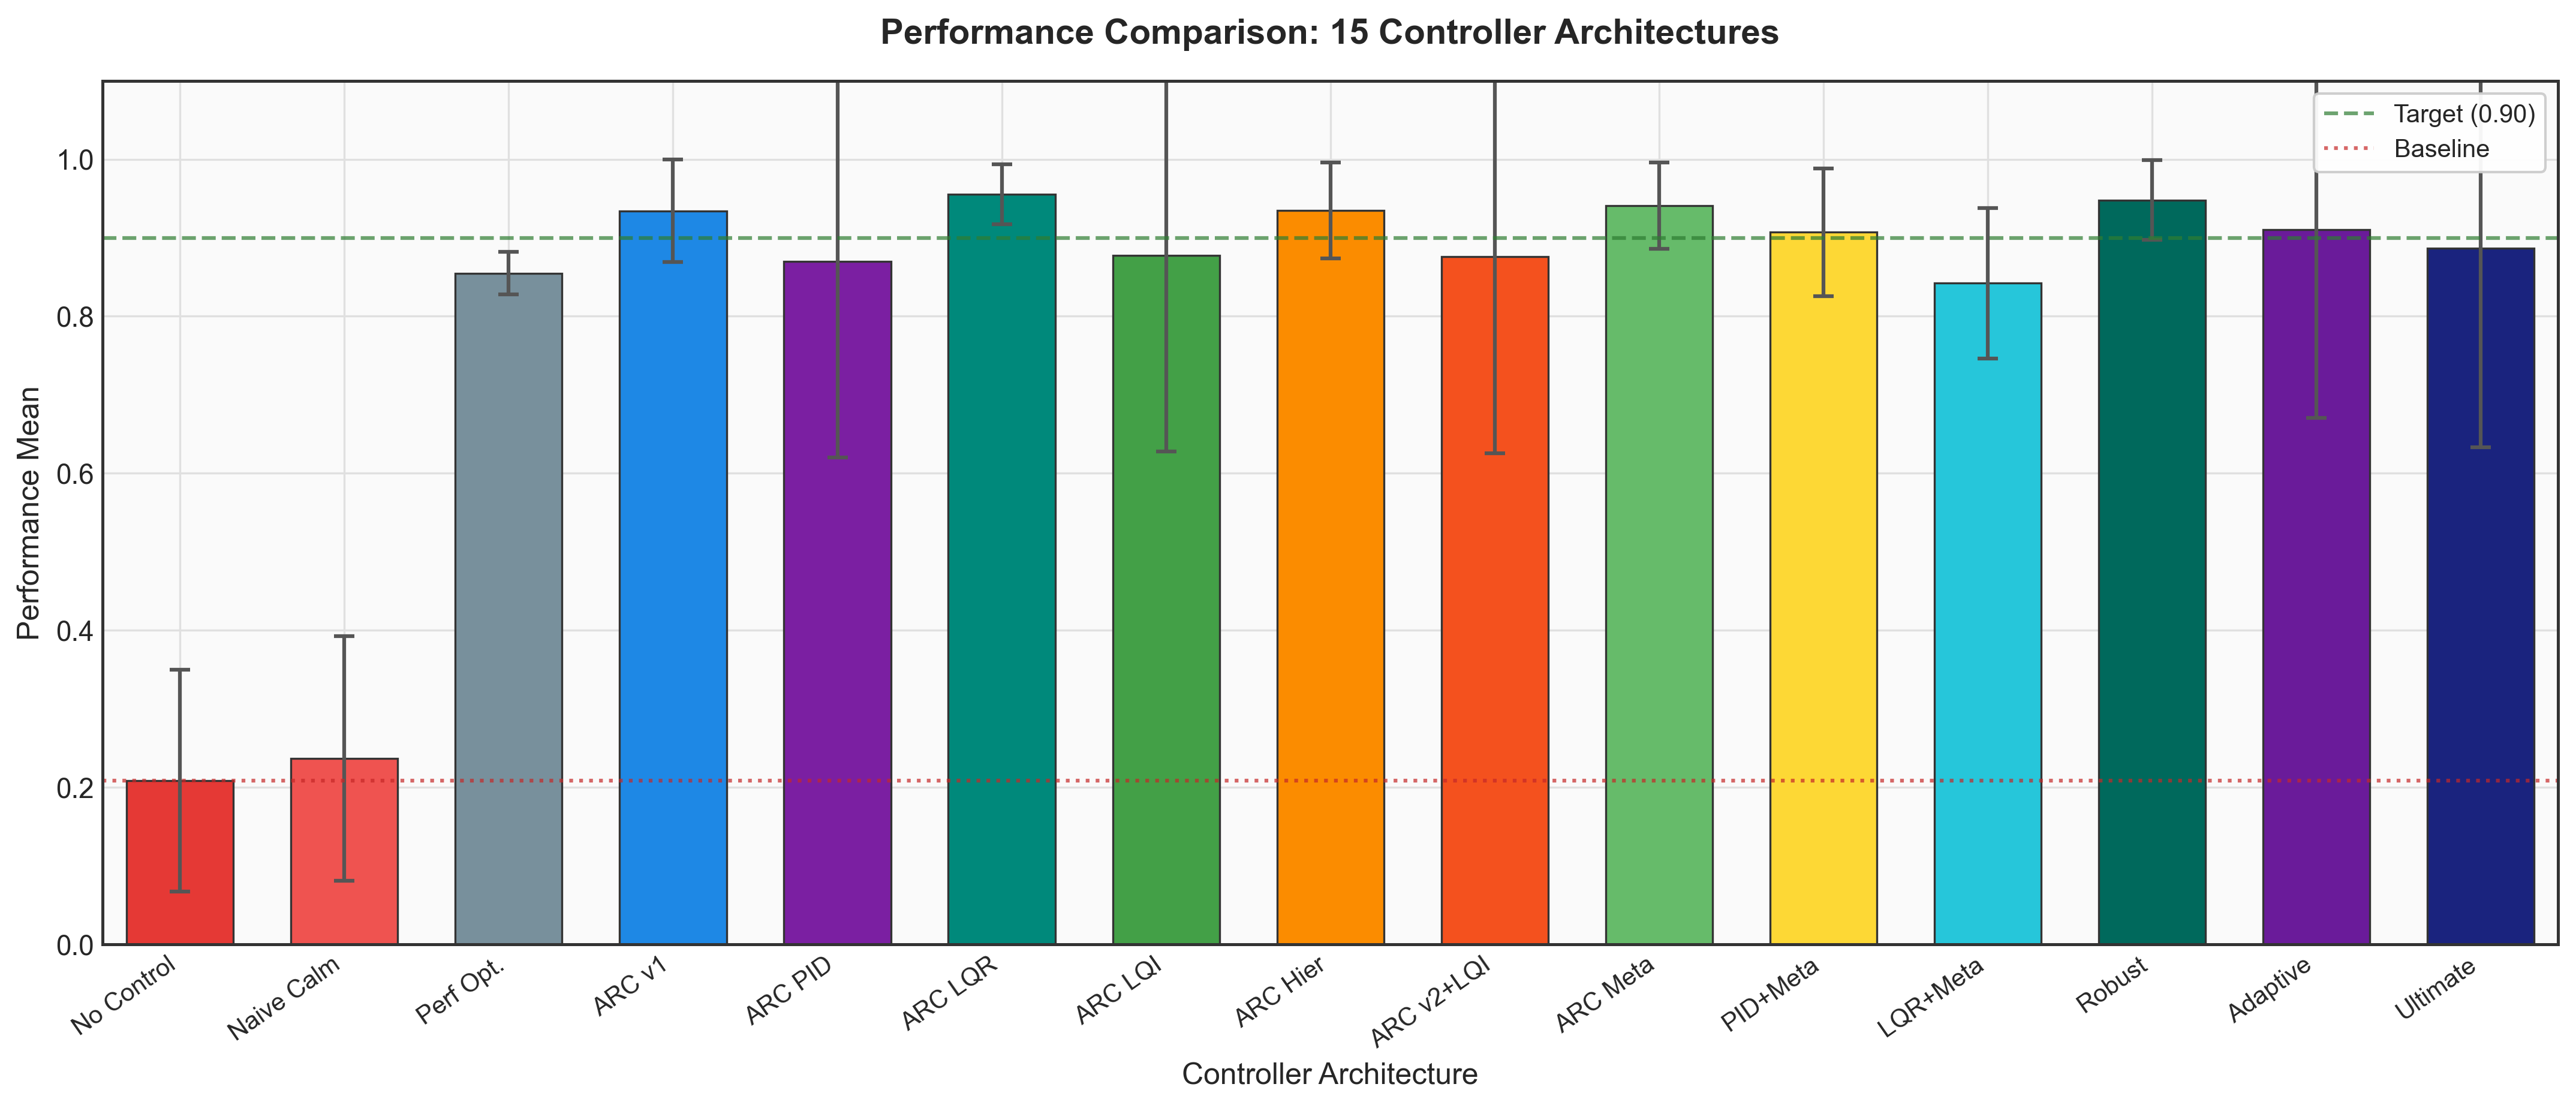
\includegraphics[width=0.48\textwidth]{figures/fig_controller_performance.png}
    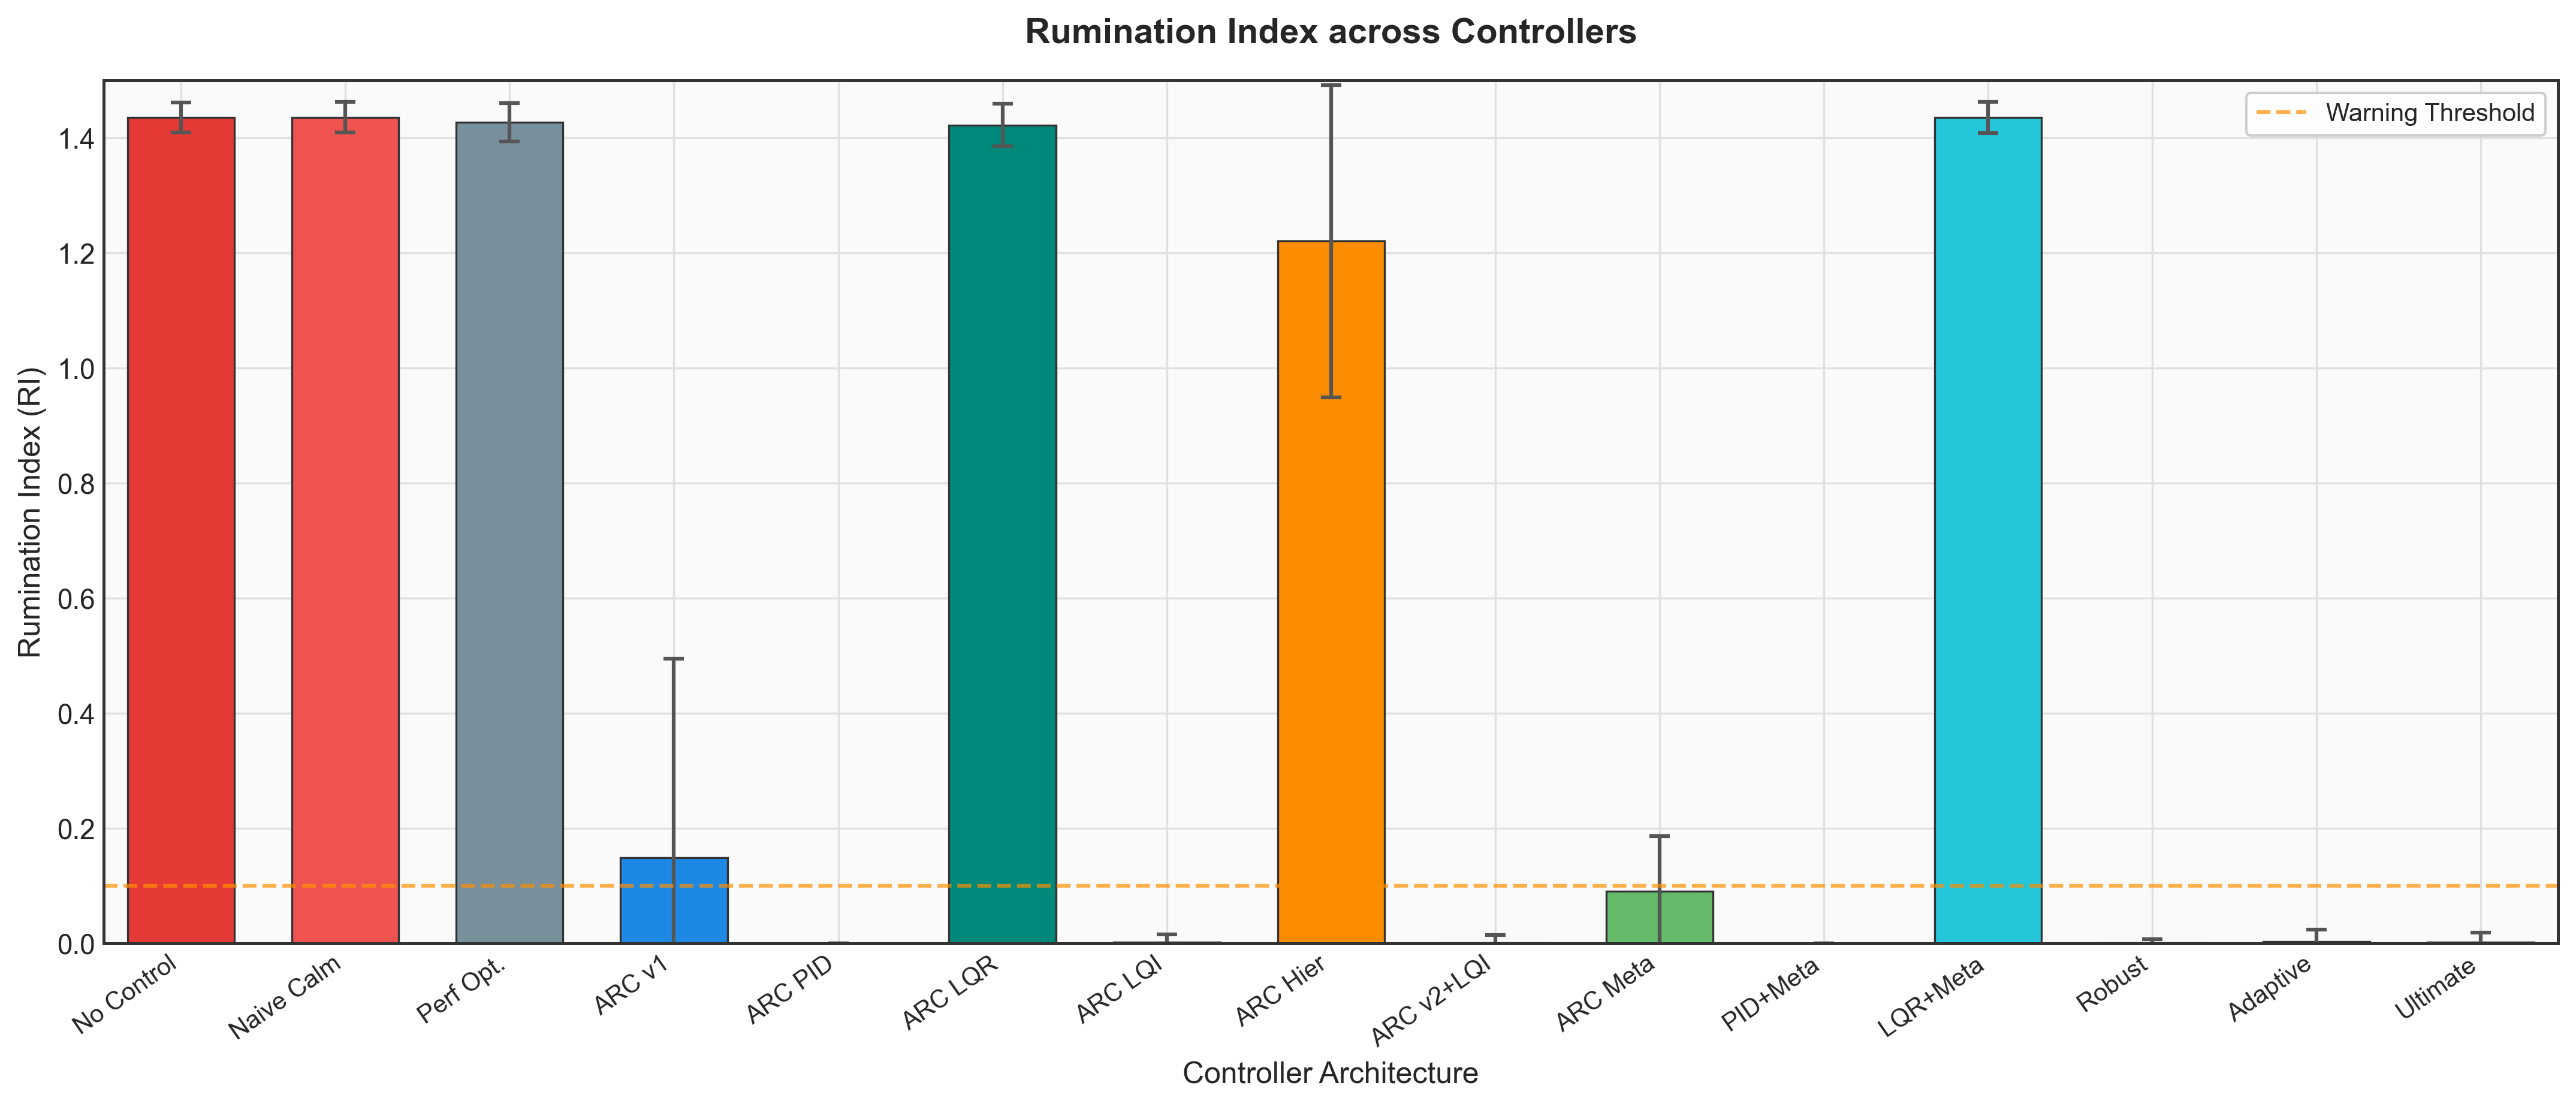
\includegraphics[width=0.48\textwidth]{figures/fig_controller_rumination.png}
    \caption{(Izquierda) PerfMean entre los 15 controladores, agregado sobre la suite de 10 escenarios (L1--L3, L5). (Derecha) Índice de Rumiación (RI) entre los mismos controladores y suite. Cada barra es la media sobre 20 semillas; las figuras buscan mostrar patrones de orden grueso (qué familias de controlador dominan cada eje) más que valores exactos por-celda, que se dan numéricamente en la Tabla~\ref{tab:controller_comparison} y con precisión de 3 decimales en el Apéndice~G. Los lectores que necesiten auditar valores específicos deben consultar las tablas; las figuras son un resumen visual.}
    \label{fig:perf_rum}
\end{figure}
\FloatBarrier

\begin{figure}[htbp]
    \centering
    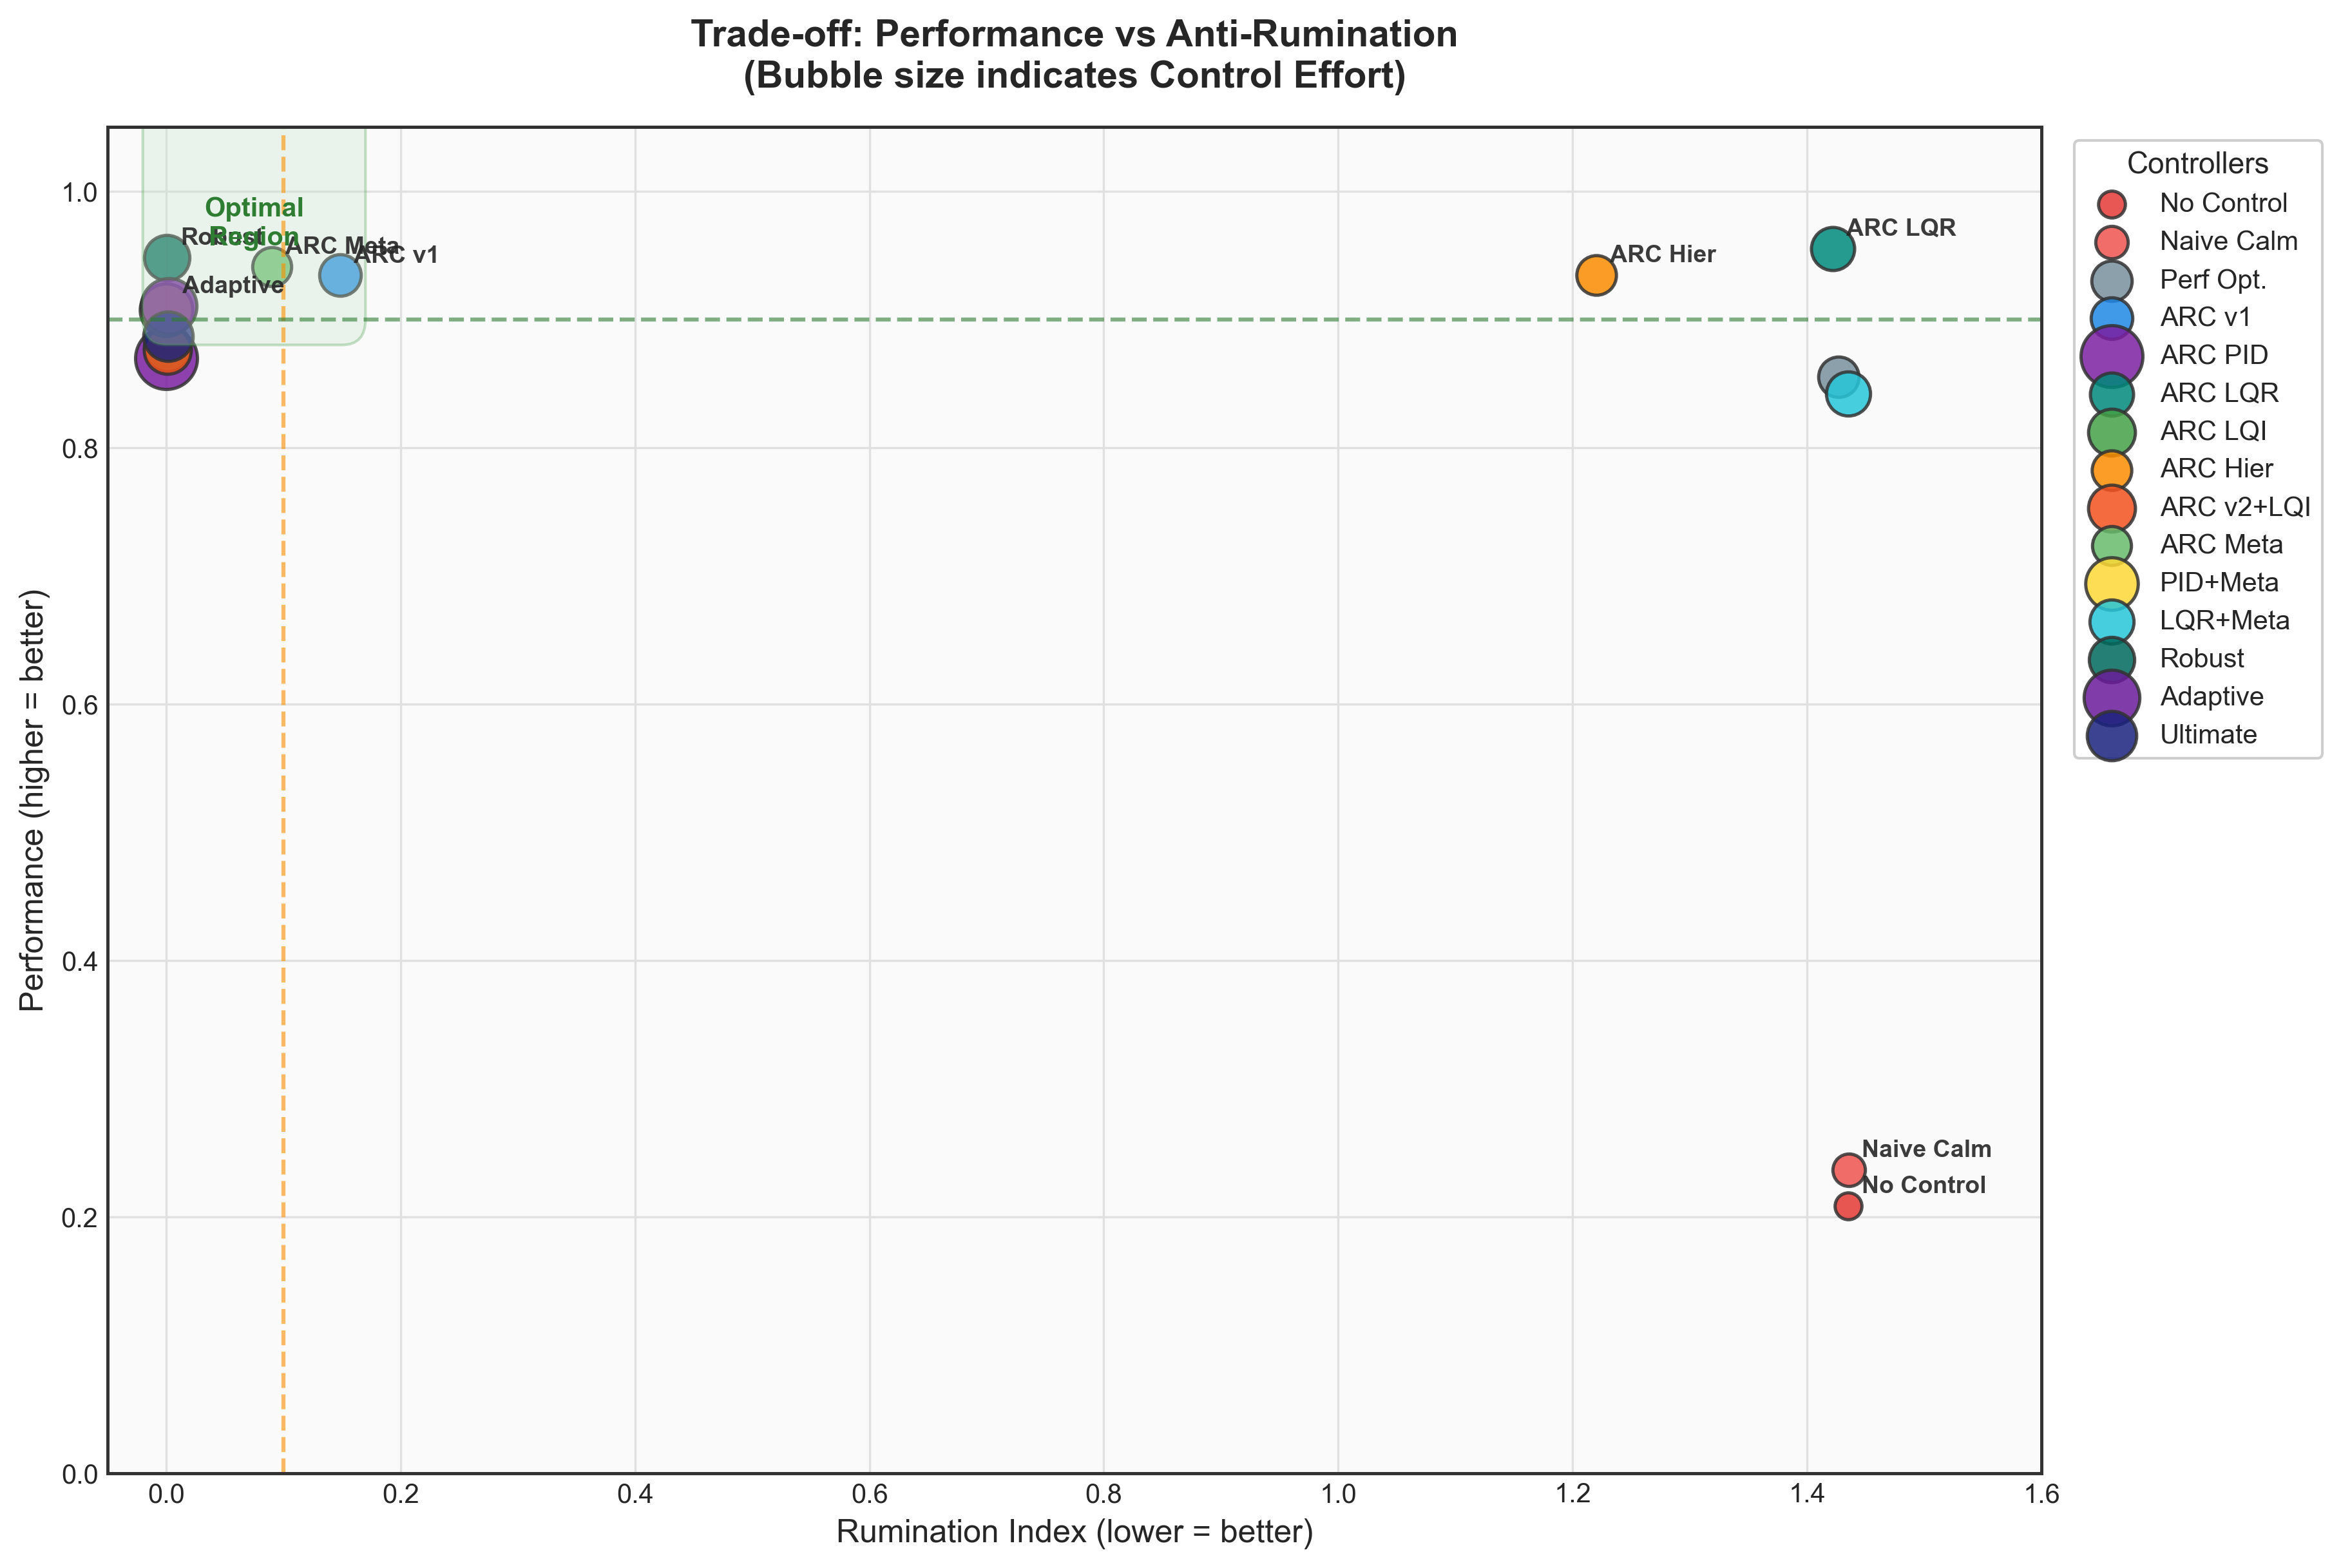
\includegraphics[width=0.48\textwidth]{figures/fig_controller_tradeoff.png}
    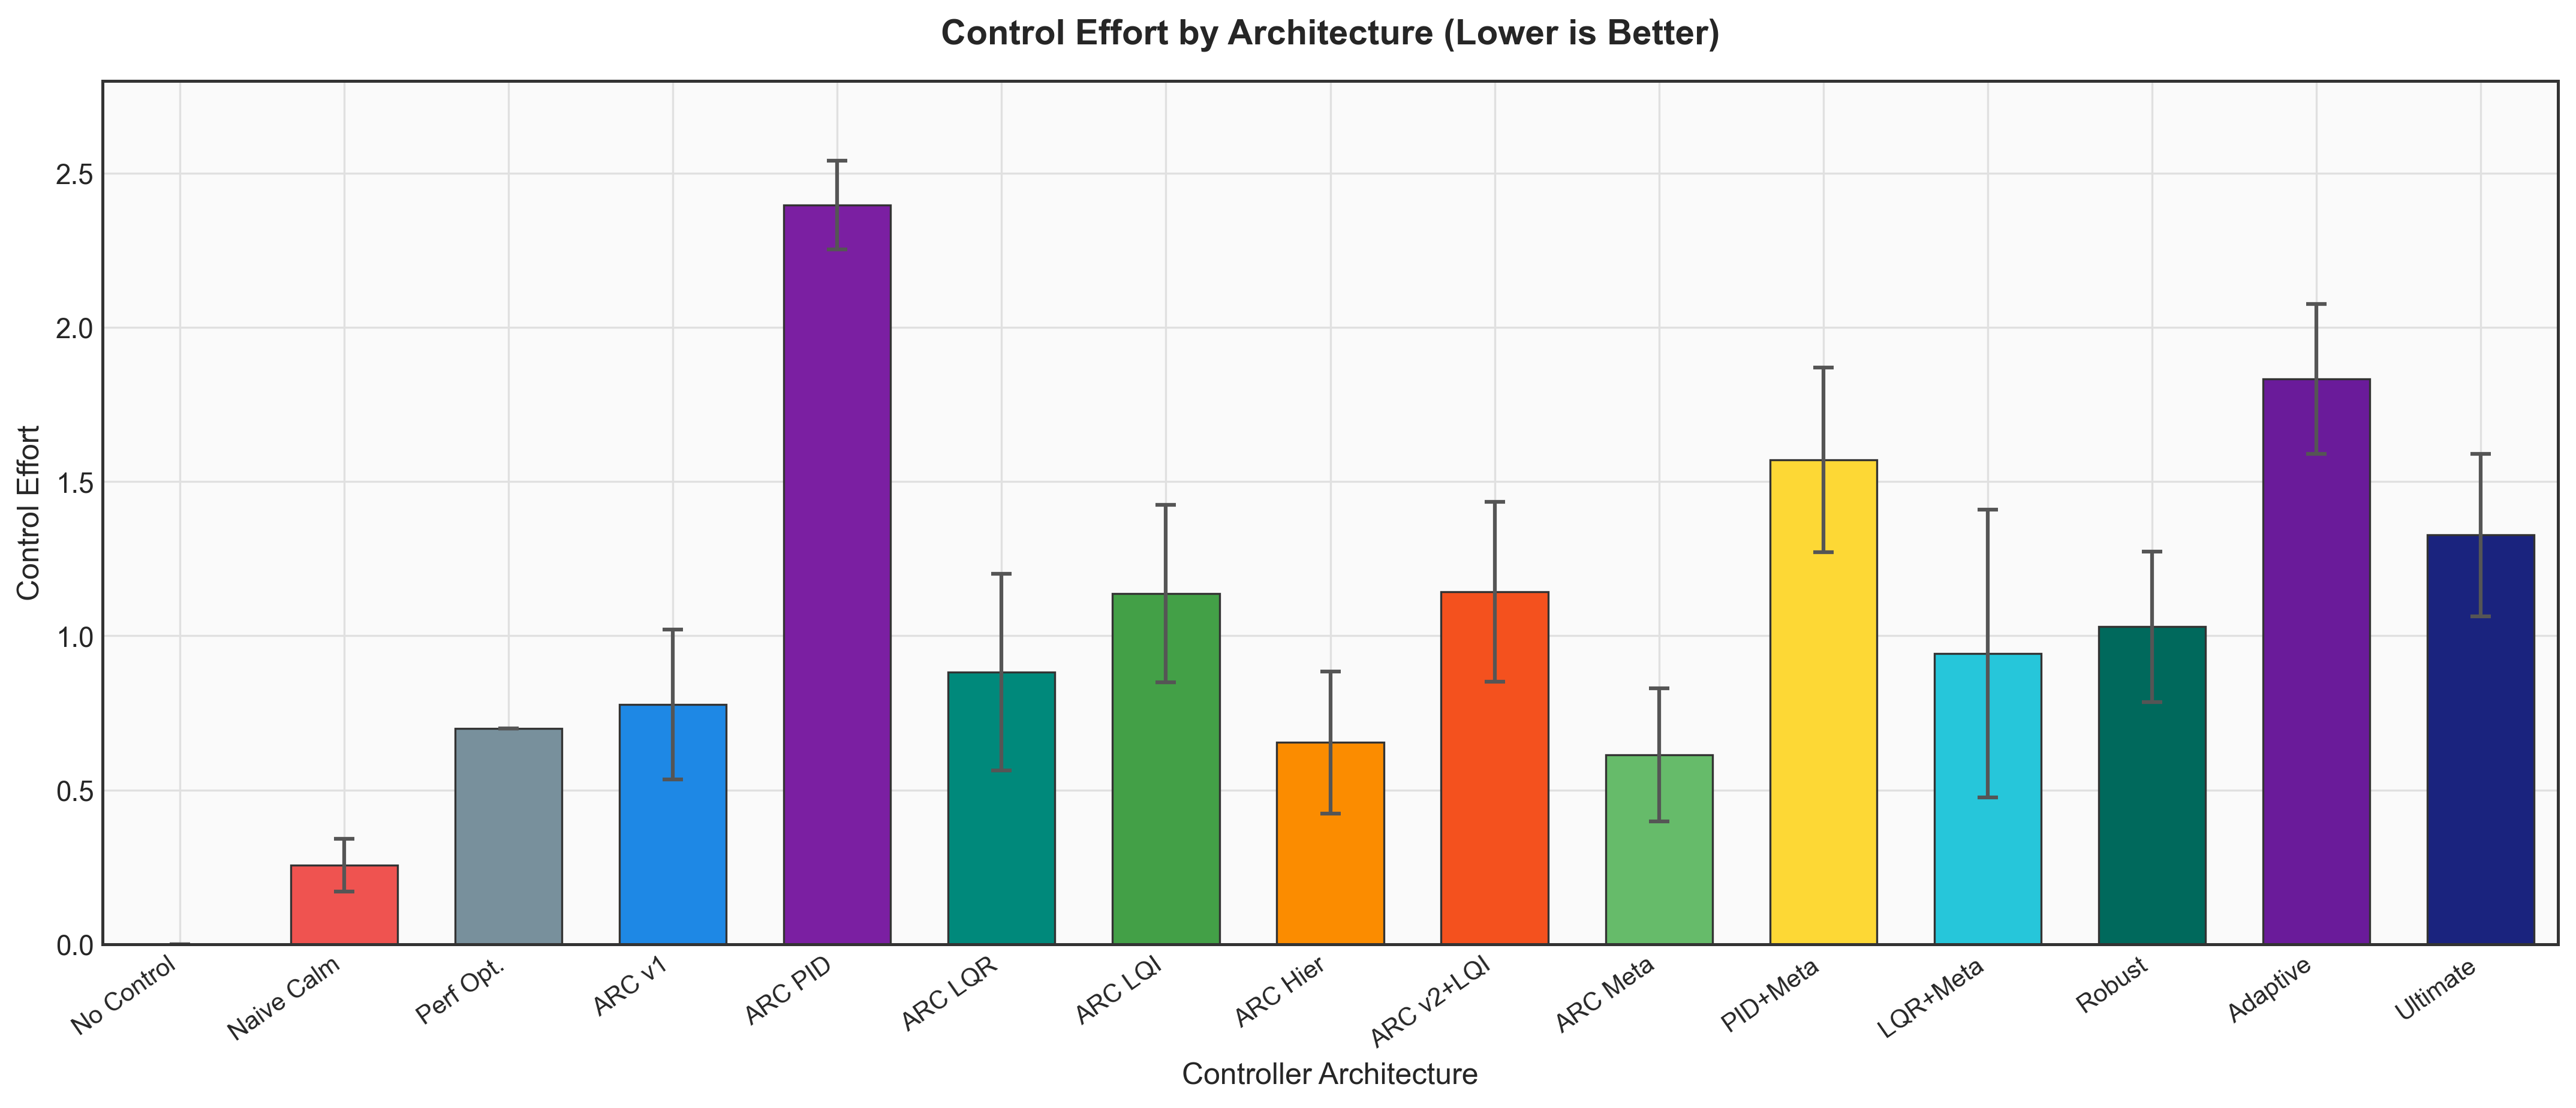
\includegraphics[width=0.48\textwidth]{figures/fig_controller_effort.png}
    \caption{(Izquierda) Trade-off entre desempeño y anti-rumiación; los puntos son los 15 controladores, los ejes son PerfMean agregado y $-\text{RI}$, de modo que la esquina superior-derecha representa simultáneamente alto desempeño y baja rumiación. El frente de Pareto informal (H$\infty$ Robust, ARC Ultimate, variantes LQI) es visible pero esta es una observación visual, no una frontera de Pareto ajustada. (Derecha) Comparación de ControlEffort entre los 15 controladores. Nota: \texttt{arc\_v3\_meta} alcanza el menor esfuerzo entre los controladores ARC \textit{efectivos} (0.61); \texttt{naive\_calm} tiene menor esfuerzo crudo (0.26) pero desempeño negligible (0.24). Valores exactos en las Tablas~\ref{tab:l4_results},~\ref{tab:controller_comparison}.}
    \label{fig:tradeoff_effort}
\end{figure}
\FloatBarrier

\begin{figure}[htbp]
    \centering
    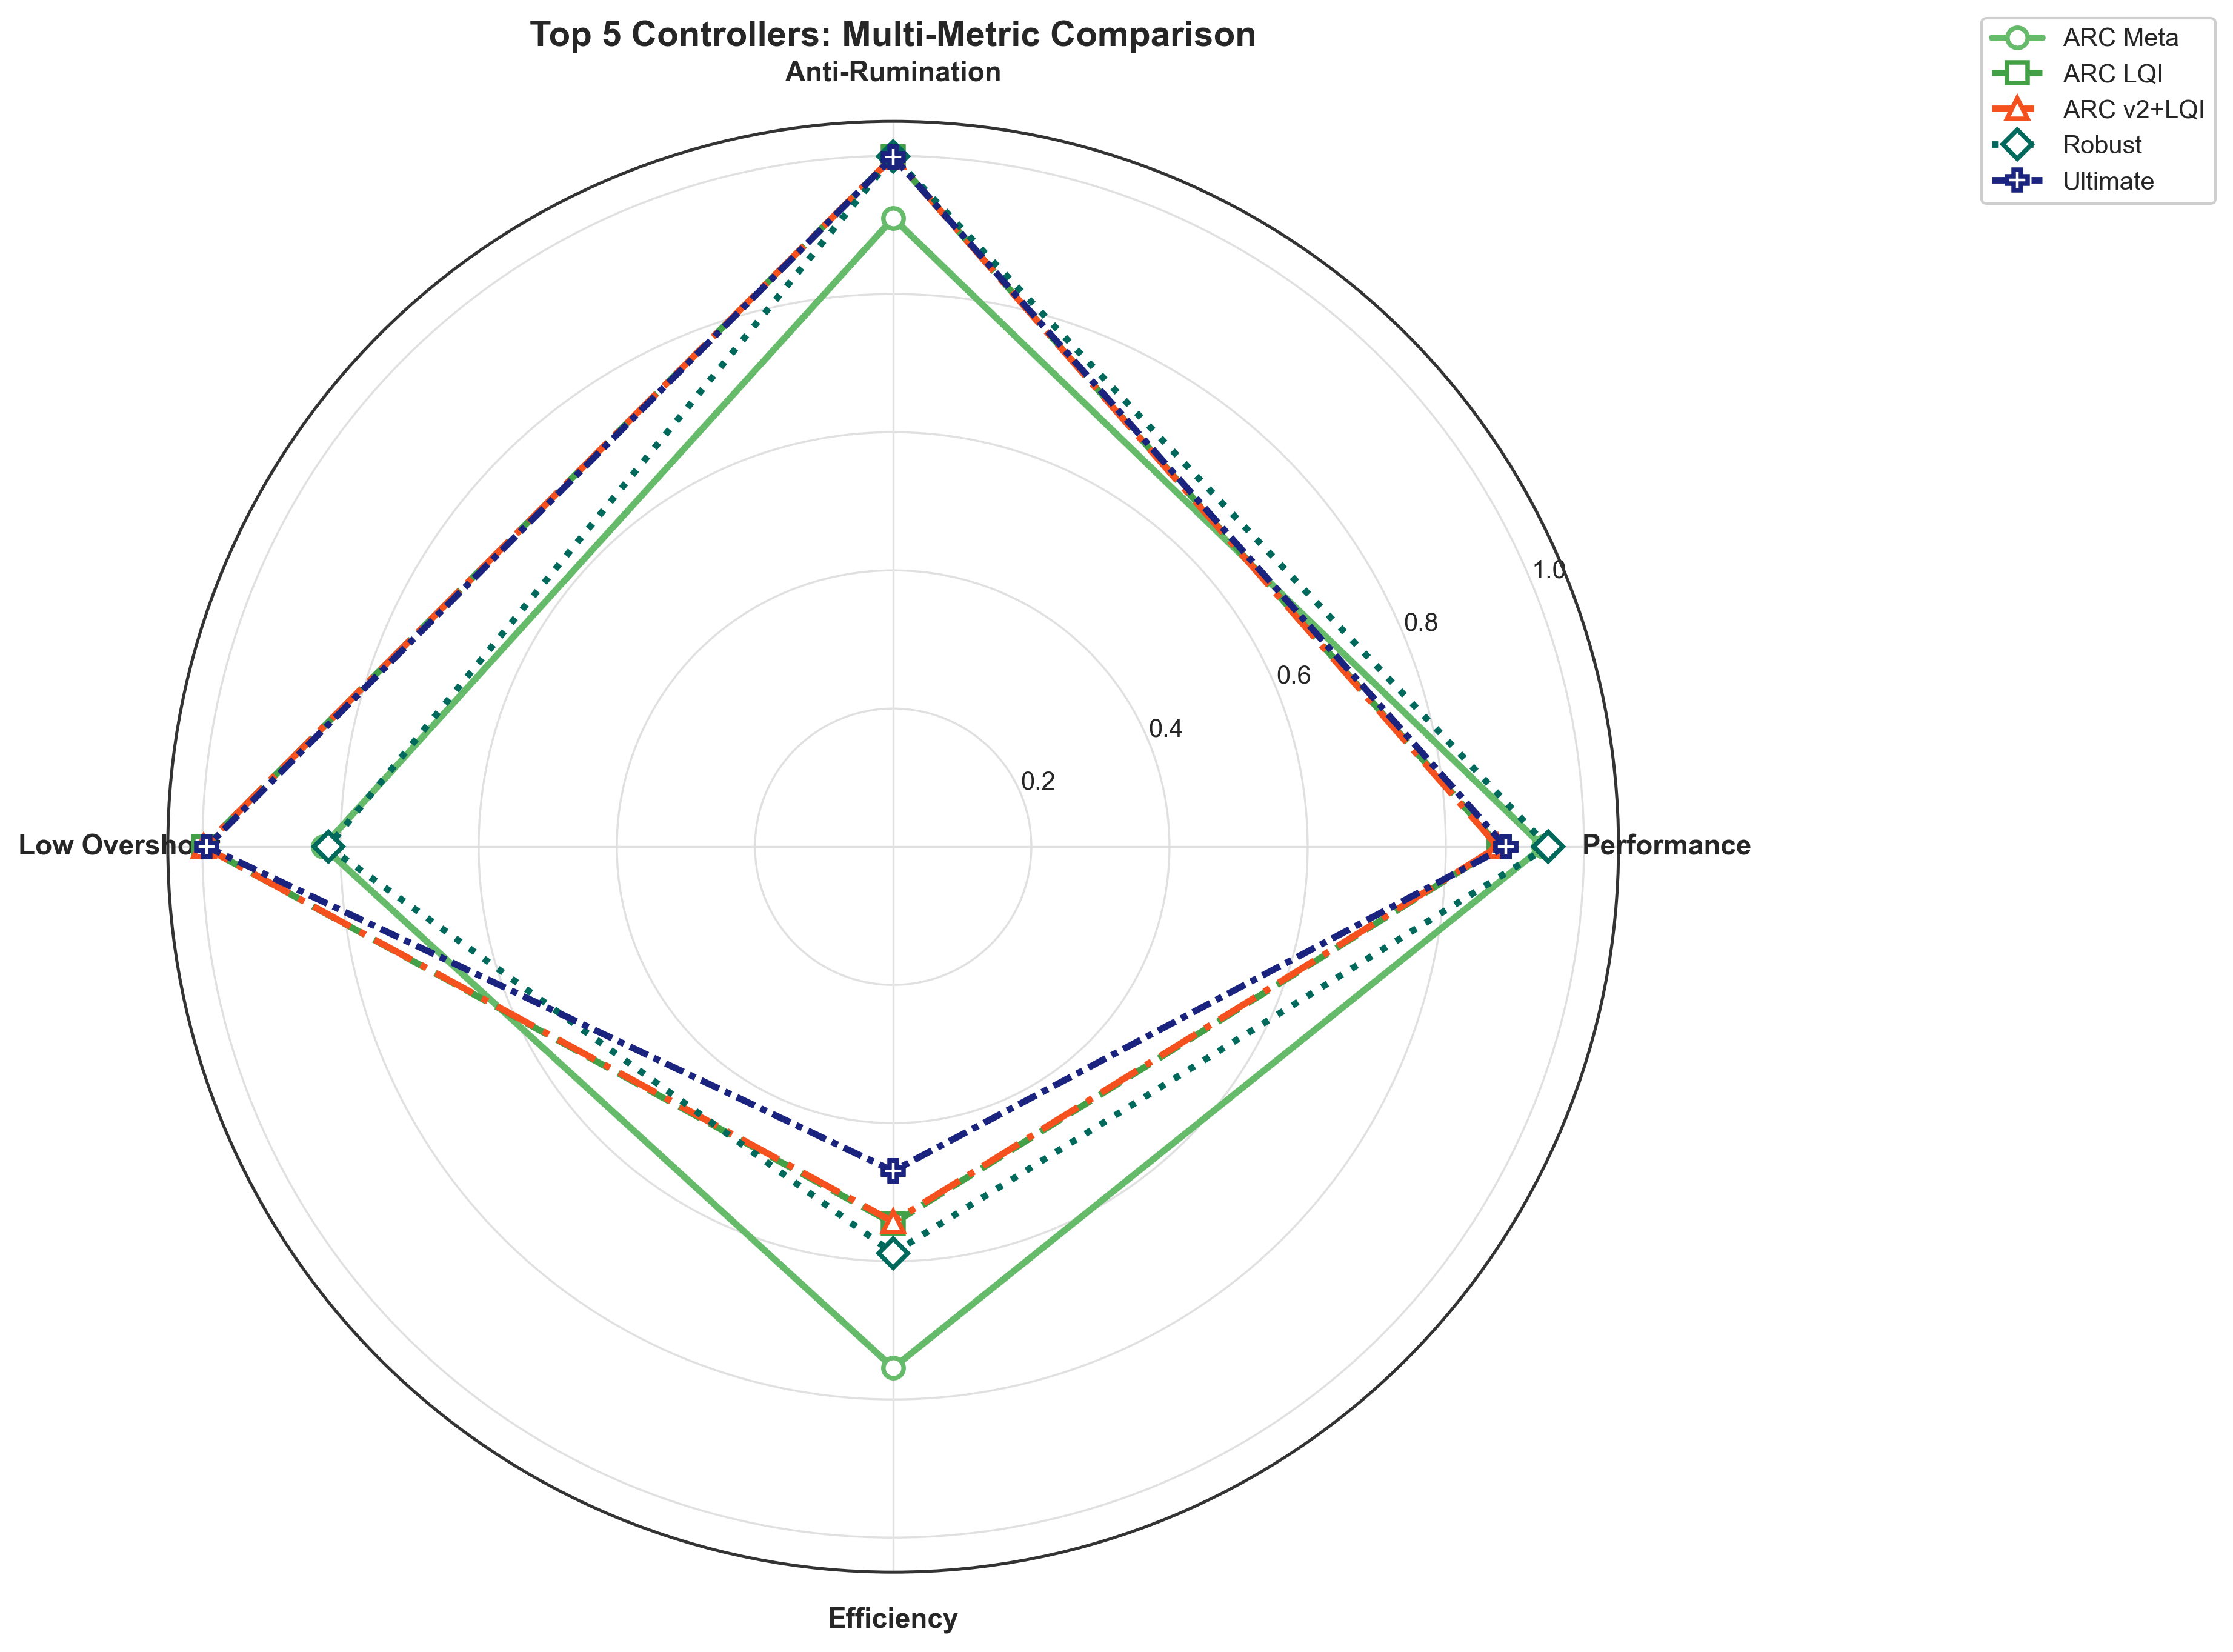
\includegraphics[width=0.72\textwidth]{figures/fig_controller_radar.png}
    \caption{Comparación multi-dimensional de los 5 mejores controladores sobre métricas agregadas (PerfMean, $-$RI, $-$RT, $-$Overshoot). \texttt{arc\_robust} alcanza el polígono más grande en esta vista agregada. \texttt{arc\_ultimate} también se ve fuerte en los ejes agregados, pero esta es una vista promediada sobre la suite de 10 escenarios y oculta dos hechos importantes: (i) su ControlEffort agregado (1.33) está entre los más altos de los 15 controladores, así que no es ``casi-óptimo en eficiencia''; (ii) colapsa en \texttt{adversarial\_coupling} (PerfMean $=0.134$, véase Tabla~\ref{tab:g10_adversarial_coupling}) debido al windup integral. Esta vista de radar, por lo tanto, debe leerse como un resumen agregado, no como un reclamo de robustez entre todos los escenarios; el test de tres criterios en la Tabla~\ref{tab:three_criterion_test} es la declaración definitiva sobre consistencia.}
    \label{fig:radar}
\end{figure}
\FloatBarrier

\section{Discusión}

\subsection{Interpretación}

Nuestros resultados soportan la hipótesis de que \textbf{los agentes con estados afectivos internos requieren regulación explícita}. Sin regulación, las perturbaciones causan fallas en cascada---el arousal impulsa la ganancia narrativa hacia la saturación, degradando el desempeño en un bucle tipo-rumiación.

ARC rompe este bucle mediante:
\begin{enumerate}
    \item \textbf{Monitoreo proporcional del riesgo} (incertidumbre, arousal, narrativa)
    \item \textbf{Supresión DMN} (anti-rumiación)
    \item \textbf{Memory gating} (protege el conocimiento aprendido bajo estrés)
    \item \textbf{Programación de ganancia} (asignación eficiente de recursos)
\end{enumerate}

\subsection{Implicaciones para la Seguridad en IA}

El presente estudio valida ARC en un entorno restringido: un espacio de estados simulado de 10 dimensiones (L1--L5) y dos variantes tabulares de GridWorld (L6). Dentro de ese entorno, observamos tres modos de falla concretos que las dinámicas afectivas no controladas exhiben y que la regulación de lazo cerrado mitiga:
\begin{itemize}
    \item \textbf{Bucles de rumiación:} procesamiento perseverativo, capturado aquí por el Índice de Rumiación en L3 / L5;
    \item \textbf{Desestabilización inducida por estrés:} perturbaciones externas que producen intensidad narrativa sostenida por encima del umbral, capturada por el colapso de PerfMean en los baselines L1--L3;
    \item \textbf{Sobreescritura de memoria bajo cambio:} olvido catastrófico cuando los cambios de distribución no se compuertan, capturado por la métrica de Retention en L2.
\end{itemize}
\emph{Hipotetizamos} que modos de falla análogos aplicarían a futuros sistemas de IA que mantengan estados afectivos internos persistentes, y que la regulación de lazo cerrado de esos estados es un mitigante candidato; pero esta generalización está más allá del alcance de lo que los experimentos actuales demuestran. El alcance directo de nuestra evidencia es el benchmark ASSB y el wrapper tabular L6 --- la extensión a deep RL, a agentes basados en modelos de lenguaje y a sistemas con dinámicas internas más realistas (no-lineales, multi-escala, alta dimensión) es trabajo futuro, y la falla de escalabilidad observada en la suite DQN L6b (Apéndice~\ref{sec:dqn_suite}) es un recordatorio explícito de que la transferencia directa no se asume.

\subsection{Trade-offs entre desempeño, estabilidad y complejidad}

Nuestro análisis profundo reveló cuatro insights críticos:

\textbf{1. El trade-off regulación--desempeño.} La comparación entre controladores proporcionales (ARC v1, PerfMean=0.93) y controladores integrales (PID, PerfMean=0.87) revela que eliminar completamente la rumiación (RI=0) tiene un costo de aproximadamente 6 puntos porcentuales en desempeño bruto (Tabla~\ref{tab:controller_comparison}). Este es el trade-off clásico de la teoría de control entre rechazo de perturbaciones (acción integral) y desempeño nominal: los controladores tolerantes al riesgo (proporcionales) pueden sobresalir en regímenes benignos pero pierden la garantía de error estacionario cero ante perturbaciones persistentes. La advertencia crítica es que los controladores integrales son frágiles bajo acoplamiento adversarial (Sección~6.6), lo que motiva los aumentos anti-windup como el principal ítem de trabajo futuro.

\textbf{2. El verdadero ``jefe final'':} contrariamente al supuesto de que el ruido es el estresor principal, el escenario \texttt{adversarial\_coupling} demostró ser la prueba más difícil (desempeño global más bajo: 0.56). Esto implica que resistir la manipulación (entornos que incentivan estados internos peligrosos) es significativamente más difícil para los agentes que resistir incertidumbre o shocks.

\textbf{3. La trampa de la complejidad:} nuestro controlador más complejo, \texttt{arc\_ultimate} (MPC+LQI), rindió por debajo de la arquitectura más simple \texttt{arc\_robust} en el agregado de 10 escenarios (PerfMean $0.89$ vs $0.95$, ControlEffort $1.33$ vs $1.03$; véase Tabla~\ref{tab:controller_comparison}). Esto sugiere que para regulación homeostática, el control reactivo robusto es superior al modelado predictivo complejo cuando el horizonte del modelo predictivo no coincide con la escala temporal de las perturbaciones---``más inteligente'' no siempre es más seguro.

\textbf{4. La paradoja de la adaptación:} \texttt{arc\_adaptive} muestra fuerte sensibilidad al contexto: queda casi en el techo en shocks de alta varianza (\texttt{reward\_flip}: 0.998; \texttt{noise\_burst}: 0.998) pero colapsa en \texttt{adversarial\_coupling} (0.193). Esto es consistente con la limitación clásica de \textbf{persistencia de excitación} \cite{Astrom2008}: los estimadores adaptativos requieren variación informativa y pueden volverse frágiles bajo regímenes adversariales con recompensa mal alineada.

\subsection{Limitaciones}

\begin{enumerate}
    \item \textbf{Dinámicas simplificadas:} nuestro modelo de espacio de estados de 10 dimensiones abstrae la complejidad de las interacciones neuroquímicas reales. Los sistemas afectivos biológicos involucran dinámicas no-lineales, estocásticas y multi-escala que nuestras aproximaciones lineales no capturan por completo. Amenazas a la validez externa: (i) bajo dinámicas fuertemente no-lineales, el resultado de rechazo por acción integral (Lema~1) ya no garantiza error estacionario cero porque el equilibrio de lazo cerrado puede bifurcarse o dejar de existir, así que el hallazgo de RI = 0 en L1--L3 no debe leerse como una propiedad genérica del ARC integral; (ii) bajo mayor estocasticidad (p.\ ej.\ ruido multiplicativo o perturbaciones de cola pesada) se espera que la falla por windup que observamos bajo \texttt{adversarial\_coupling} aparezca antes y en más escenarios, ya que la probabilidad de saturación crece con la varianza de la perturbación; (iii) en sistemas multi-escala, el integrador de escala lenta y la acción proporcional de escala rápida pueden interactuar destructivamente, un régimen no ejercido por ASSB. Los hallazgos reportados aquí deben interpretarse, por lo tanto, como evidencia de que los mecanismos funcionan en un entorno \emph{acotado, de baja dimensión, cuasi-lineal} que sirve como andamio para estudio adicional, no como validación de ARC sobre dinámicas realistas a escala del sistema nervioso.
    \item \textbf{Escalabilidad a Deep RL:} la validación RL primaria de ARC usa Q-learning tabular. Nuestros experimentos exploratorios con DQN (Apéndice G.7) muestran que la transferencia directa de los mecanismos de ARC a deep RL incurre en una penalización de desempeño, indicando que la compuerta de actualizaciones y la modificación del replay requieren rediseño arquitectónico para aprendices basados en gradiente. La extensión a PPO, A3C o modelos de lenguaje grandes con estados tipo-afecto emergentes permanece como un desafío abierto.
    \item \textbf{Complejidad del entorno:} L6 se valida en variantes de GridWorld. Aunque estas capturan desafíos clave de no-estacionariedad, los entornos del mundo real (Atari, robótica) introducen problemas adicionales visuales y de observabilidad.
    \item \textbf{Validez interna (Ablación L6):} Nuestro estudio de ablación (Sección 6.7) muestra que el memory gating solo alcanza la mayor tasa de éxito individual (71.8\%), mientras que combinar ambos mecanismos reduce el desempeño global a 59.8\%. Hipotetizamos una interacción sub-aditiva entre los dos componentes pero no la testeamos causalmente en este trabajo. El +49.8\% reportado corresponde al wrapper completo relativo al baseline, no al mejor componente ablacionado individualmente.
    \item \textbf{Sensibilidad al umbral:} aunque robusto en un amplio rango ($a_{safe}, s_{safe} \in [0.4, 0.8]$) en el escenario \texttt{reward\_flip}, los umbrales de seguridad aún requieren ajuste contextual. El ajuste automático permanece como una dirección futura prometedora.
\end{enumerate}

\subsection{Trabajo Futuro}\label{sec:future_work}

\begin{enumerate}
    \item \textbf{Control anti-windup e integral robusto.} El modo de falla por windup integral identificado bajo \texttt{adversarial\_coupling} (Sección~6.6) es un tema clásico de la teoría de control con remedios bien entendidos (clamping, back-calculation, integración condicional). Integrarlos en ARC v1 PID / LQI y re-evaluar en L5 es el siguiente paso de mayor prioridad.
    \item \textbf{Integración con Deep RL vía modulación suave.} Rediseñar los mecanismos de ARC para aprendices basados en gradiente (DQN, PPO), reemplazando la compuerta dura con modulación suave (escalamiento de learning rate, re-ponderación de loss), informados por los modos de falla identificados en el Apéndice~\ref{sec:dqn_suite}.
    \item \textbf{Controladores aprendidos.} Entrenar políticas con redes neuronales para regulación, usando los controladores clásicos de este artículo como demostraciones expertas.
    \item \textbf{Escalar a robótica.} Validación en MuJoCo o manipuladores físicos (p.\ ej., UR5), donde ARC opera como un regulador cognitivo de Capa 3 sobre una pila sensoriomotora.
    \item \textbf{Monitoreo afectivo en LLMs.} Regular estados tipo-afecto emergentes en agentes cognitivos basados en modelos de lenguaje. Un manuscrito companion próximo \cite{Damian2026b} reporta un despliegue de ARC Robust como wrapper homeostático alrededor de un agente cognitivo vivo (OMEGA Gen 3.0); lo mencionamos como la extensión inmediata que estamos persiguiendo, no como evidencia usada para soportar los claims del presente artículo.
    \item \textbf{Análisis formal de estabilidad.} Extender el Lema~1 al sistema no-lineal completo de lazo cerrado vía métodos de Lyapunov, como prerrequisito para despliegue en entornos de alto riesgo.
    \item \textbf{Alineación humano--IA.} Usar el memory-gating y la prevención de deriva de valor de ARC como bloques de construcción para alineación de largo horizonte.
\end{enumerate}

\subsection{Declaración de Ética e Impacto Amplio}

Este trabajo aborda la seguridad y estabilidad de sistemas de IA que incorporan estados afectivos internos. \textbf{Beneficios potenciales:} sistemas de IA más seguros, menos propensos a fallas impredecibles; mejor robustez. \textbf{Riesgos potenciales:} si se usan para manipulación, los agentes regulados podrían ser más difíciles de perturbar; la terminología ``afectiva'' podría invitar al antropomorfismo.

\section{Conclusión}

Presentamos ARC, un marco de control homeostático para agentes con estados afectivos internos, y ASSB, un benchmark para evaluar la estabilidad afectiva. Nuestros experimentos demuestran:
\begin{enumerate}
    \item \textbf{Los estados afectivos sin regulación llevan al colapso} (PerfMean $\leq$ 0.30 en escenarios de estabilidad L1 vs.\ 0.966 para ARC); los controladores integrales llevan la rumiación cerca de cero a un costo de desempeño modesto, pero con fragilidad adversarial.
    \item \textbf{El meta-control reduce el esfuerzo mientras preserva el desempeño} ($-$20.9\% de ControlEffort agregado, $+0.7\%$ de PerfMean agregado; direccional, sin test paramétrico).
    \item \textbf{ARC se asocia con mayor éxito de transferencia en aprendizaje tabular RL en el único entorno no saturado} de la suite L6 (\texttt{ChangingGoalGridWorld}: $39.9\% \rightarrow 59.8\%$, $+49.8\%$ relativo; los otros dos entornos L6 están en el techo del 100\% para ambas condiciones). Una ablación aísla al memory gating como el mecanismo individual más fuerte ($71.8\%$, $+79.9\%$ relativo sobre el baseline), con evidencia de interacción sub-aditiva cuando se compone con detección de cambio. Presentamos todos los resultados de L6 como direccionales, no testeados por hipótesis. La integración con Deep RL (DQN) rinde por debajo del DQN baseline (Apéndice~\ref{sec:dqn_suite}) y se reporta transparentemente como un límite de alcance que requiere rediseño arquitectónico.
    \item \textbf{Los controladores integrales son frágiles bajo acoplamiento adversarial}, colapsando por debajo del baseline debido al windup---los controladores robustos o proporcionales son preferibles para entornos adversariales. Los aumentos anti-windup (un remedio estándar en control clásico) se identifican como la línea de trabajo futuro más prometedora.
\end{enumerate}

Este trabajo abre direcciones para control aprendido, integración con algoritmos modernos de RL y aplicación a sistemas de IA del mundo real con componentes afectivos.

\begin{thebibliography}{99}

\bibitem{Achiam2017}
Achiam, J., Held, D., Tamar, A., \& Abbeel, P. (2017). Constrained Policy Optimization. ICML 2017, 22--31. arXiv:1705.10528.

\bibitem{Altman1999}
Altman, E. (1999). Constrained Markov Decision Processes. Chapman \& Hall/CRC.

\bibitem{Amodei2016}
Amodei, D., et al. (2016). Concrete problems in AI safety. arXiv:1606.06565.

\bibitem{Astrom2008}
{\AA}str\"om, K.J. \& Murray, R.M. (2008). Feedback Systems: An Introduction for Scientists and Engineers. Princeton University Press.

\bibitem{Baars1988}
Baars, B.J. (1988). A Cognitive Theory of Consciousness. Cambridge University Press.

\bibitem{Buckner2008}
Buckner, R.L., Andrews-Hanna, J.R. \& Schacter, D.L. (2008). The brain's default network: anatomy, function, and relevance to disease. Annals of the New York Academy of Sciences, 1124(1), 1--38.

\bibitem{Carver1982}
Carver, C.S. \& Scheier, M.F. (1982). Control theory: A useful conceptual framework for personality-social, clinical, and health psychology. Psychological Bulletin, 92(1), 111--135.

\bibitem{Damasio1994}
Damasio, A.R. (1994). Descartes' Error: Emotion, Reason, and the Human Brain. G.P. Putnam's Sons.

\bibitem{Damian2026b}
Dami\'{a}n Reynoso, J.E. (2026b). \emph{Embodied Affective Regulation: Deploying the Affective Regulation Core in a Live LLM-Based Cognitive Agent}. Manuscrito companion al presente trabajo, por aparecer en TechRxiv; el identificador persistente se agregará a esta entrada bibliográfica una vez emitido.

\bibitem{Friston2010}
Friston, K. (2010). The free-energy principle: a unified brain theory? Nature Reviews Neuroscience, 11(2), 127--138.

\bibitem{Garcia2015}
Garcia, J. \& Fern\'andez, F. (2015). A comprehensive survey on safe reinforcement learning. Journal of Machine Learning Research, 16, 1437--1480.

\bibitem{Gross1998}
Gross, J.J. (1998). The emerging field of emotion regulation: An integrative review. Review of General Psychology, 2(3), 271--299.

\bibitem{Hamilton2015}
Hamilton, J.P., Farmer, M., Fogelman, P. \& Gotlib, I.H. (2015). Depressive rumination, the default-mode network, and the dark matter of clinical neuroscience. Biological Psychiatry, 78(4), 224--230.

\bibitem{Hebb1955}
Hebb, D.O. (1955). Drives and the C.N.S. (conceptual nervous system). Psychological Review, 62(4), 243--254.

\bibitem{Ji2023}
Ji, J., et al. (2023). Safety-Gymnasium: A Unified Safe Reinforcement Learning Benchmark. arXiv:2310.12567.

\bibitem{Keramati2014}
Keramati, M. \& Gutkin, B. (2014). Homeostatic reinforcement learning for integrating reward collection and physiological stability. eLife, 3:e04811.

\bibitem{Leike2017}
Leike, J., Martic, M., Krakovna, V., Ortega, P.A., Everitt, T., Lefrancq, A., Orseau, L., \& Legg, S. (2017). AI Safety Gridworlds. arXiv:1711.09883.

\bibitem{LopezPaz2017}
Lopez-Paz, D., \& Ranzato, M.\ (2017). Gradient Episodic Memory for Continual Learning. In \emph{Advances in Neural Information Processing Systems 30} (NIPS 2017), 6467--6476. arXiv:1706.08840.

\bibitem{Lucas2004}
Lucas, C., Shahmirzadi, D., \& Sheikholeslami, N. (2004). Introducing Belbic: Brain Emotional Learning Based Intelligent Controller. Intelligent Automation \& Soft Computing, 10(1), 11--21.

\bibitem{Moerland2018}
Moerland, T.M., Broekens, J., \& Jonker, C.M. (2018). Emotion in reinforcement learning agents and robots: a survey. Machine Learning, 107(2), 443--480.

\bibitem{Ochsner2005}
Ochsner, K.N. \& Gross, J.J. (2005). The cognitive control of emotion. Trends in Cognitive Sciences, 9(5), 242--249.

\bibitem{Picard1997}
Picard, R.W. (1997). Affective Computing. MIT Press.

\bibitem{Raichle2001}
Raichle, M.E., et al. (2001). A default mode of brain function. Proceedings of the National Academy of Sciences, 98(2), 676--682.

\bibitem{Ray2019}
Ray, A., Achiam, J., \& Amodei, D. (2019). Benchmarking Safe Exploration in Deep Reinforcement Learning. arXiv:1910.01708.

\bibitem{Russell1980}
Russell, J.A. (1980). A circumplex model of affect. Journal of Personality and Social Psychology, 39(6), 1161--1178.

\bibitem{Scherer2010}
Scherer, K.R., B\"anziger, T., \& Roesch, E. (Eds.) (2010). A Blueprint for Affective Computing: A Sourcebook and Manual. Oxford University Press.

\bibitem{Sutton2018}
Sutton, R.S. \& Barto, A.G. (2018). Reinforcement Learning: An Introduction (2nd ed.). MIT Press.


\bibitem{Tononi2008}
Tononi, G. (2008). Consciousness as integrated information: a provisional manifesto. Biological Bulletin, 215(3), 216--242.

\bibitem{Wachi2024}
Wachi, A., Shen, X., \& Sui, Y. (2024). A Survey of Constraint Formulations in Safe Reinforcement Learning. IJCAI 2024. arXiv:2402.02025.

\bibitem{Watkins1992}
Watkins, C.J.C.H. \& Dayan, P. (1992). Q-learning. Machine Learning, 8, 279--292.

\bibitem{Yerkes1908}
Yerkes, R.M. \& Dodson, J.D. (1908). The relation of strength of stimulus to rapidity of habit-formation. Journal of Comparative Neurology and Psychology, 18(5), 459--482.

\end{thebibliography}

\appendix

\section{Reproducibilidad}

Checklist de reproducibilidad:
\begin{itemize}
    \item Instalar dependencias (\texttt{pip install -r requirements.txt})
    \item Correr el benchmark de simulación L1--L5 (genera \texttt{outputs\_final/metrics.csv})
    \item Generar las figuras de comparación de controladores (escribe en \texttt{figures\_controllers/})
    \item Correr el estudio de ablación (escribe en \texttt{outputs\_ablation/})
    \item Correr la validación RL L6 (escribe en \texttt{outputs\_L6\_robust/})
    \item Generar las figuras L6 (escribe en \texttt{figures\_L6/})
\end{itemize}

Todos los experimentos pueden reproducirse con:

\begin{verbatim}
# Instalar dependencias
pip install -r requirements.txt

# L1-L5: Benchmark de simulación (15 controladores x 10 escenarios)
python experiments/run.py --config configs/v2.yaml --outdir outputs_final

# Figuras de arquitectura de controladores (Tabla 3, Figuras 6-9)
python analysis/generate_controller_figures.py

# Estudio de ablación (componentes ARC; Figura 4)
python experiments/run_ablation.py \
  --config configs/v2.yaml --outdir outputs_ablation --seeds 20

# L6: Validación RL (20 semillas)
python experiments/run_l6.py --episodes 200 --seeds 20 --outdir outputs_L6_robust

# Figuras L6 (Figura 5; Apéndice E)
python visualizations/paper_figures.py --data outputs_L6_robust --output figures_L6
\end{verbatim}

Código y datos disponibles en: \url{https://github.com/edamianreynoso/arc-assb-controller}. Los resultados reportados en este artículo corresponden al estado del repositorio etiquetado como \texttt{arc-paper-v1} (el hash del commit se insertará en la carga final); los lectores que clonen \texttt{main} después de ese punto pueden observar desviación numérica debido a cambios post-envío.

\textbf{Entorno.} Los experimentos se corrieron en Python 3.11 con los pisos de librerías declarados en \texttt{requirements.txt}: \texttt{numpy>=1.26}, \texttt{scipy>=1.11}, \texttt{pandas>=2.2}, \texttt{matplotlib>=3.8}, \texttt{seaborn>=0.13}, \texttt{pyyaml>=6.0}. El pipeline tabular-RL de L6 no tiene dependencias adicionales de librerías de aprendizaje (Q-learning simple en NumPy/SciPy). La suite exploratoria DQN L6b (Apéndice~\ref{sec:dqn_suite}) usa adicionalmente \texttt{stable-baselines3>=2.0} y \texttt{gymnasium>=0.29}. Los resultados se produjeron en CPU de consumidor (sin GPU requerida); el wall-clock L1--L5 es del orden de minutos por (controlador, escenario, 20 semillas), y el benchmark completo (15 controladores $\times$ 10 escenarios $\times$ 20 semillas) termina en pocas horas. Las semillas son deterministas y se fijan vía \texttt{configs/v2.yaml}; la lista canónica de semillas son los enteros $\{0, 1, \ldots, 19\}$ para las celdas de 20 semillas y $\{0, 1, \ldots, 9\}$ para las celdas DQN de 10 semillas.

\section{Ecuaciones de la Dinámica de Estado}

\subsection{Variables Cognitivas}

\begin{verbatim}
i(t+1) = clip(i + k_i_att * u_att - mu_i * (i - i0) - k_i_u * U_eff)
p(t+1) = clip(p - k_p_pe * PE - k_p_u * U_eff + k_p_i * i + mu_p * (p0 - p))
g(t+1) = clip(g + k_g_i * i + k_g_p * p - k_g_u * U_eff
              - k_g_a * [a - a_safe]^+ + mu_g * (g0 - g))
phi(t+1) = clip(phi + k_phi_gp * (g * p) - mu_phi * (phi - phi0))
\end{verbatim}

\subsection{Variables Afectivas}

\begin{verbatim}
s(t+1) = clip(s + k_s_u * U_eff + k_s_pe * PE - mu_s * (s - s0) - k_s_dmg * u_dmg)
a(t+1) = clip(a + k_a_pe * PE + k_a_u * U_eff + k_a_s * [s - s_safe]^+
              - mu_a * (a - a0) - k_a_calm * u_calm)
v(t+1) = clip(v + k_v_r * (R+1)/2 - k_v_pe * PE - k_v_u * U_eff
              - mu_v * (v - v0) + k_v_reapp * u_reapp)
\end{verbatim}

\subsection{Variables de Memoria}

\begin{verbatim}
M_f(t+1) = clip(M_f + w_prob * dM_f - mu_mf * (M_f - M_f0))
M_s(t+1) = clip(M_s + k_ms * M_f - mu_ms * (M_s - M_s0))

donde w_prob = sigmoid(k_w_a * a + k_w_v * abs(dv)) * u_mem
\end{verbatim}

\subsection{Incertidumbre Efectiva}

\begin{verbatim}
U_eff = clip(U_exog * (1 - k_u_att * u_att))
U(t+1) = clip(U + tau_u * (U_eff - U))
\end{verbatim}

\section{Ecuaciones de Control de ARC}

\subsection{Señal de Riesgo}

\begin{verbatim}
risk = w_U * U + w_A * [A - a_safe]^+ + w_S * [S - s_safe]^+
risk = clip(risk, 0, 1)
\end{verbatim}

\subsection{Acciones de Control (ARC v1)}

\begin{verbatim}
u_dmg  = min(1, k_dmg * risk)
u_att  = min(1, k_att * U * (1 - [A - a_safe]^+))
u_mem  = 1 - min(1, k_mem_block * risk)
u_calm = min(1, k_calm * [A - a_safe]^+)
u_reapp = min(1, k_reapp * U * (1 - risk))
\end{verbatim}

\subsection{Meta-Control (ARC v3)}

\begin{verbatim}
# Programación de ganancias
if mean_perf(last 20 steps) > target_perf:
    gain = max(0.80, gain - decay)
elif mean_perf(last 20 steps) < target_perf - 0.10:
    gain = min(1.40, gain + boost)

# Aplicar a las constantes de control
k_dmg  = base_k_dmg  * max(1.0, gain)  # Nunca relajar el control DMN
k_calm = base_k_calm * gain
k_att  = base_k_att  * gain
\end{verbatim}

\section{Definiciones de Métricas}

\subsection{Desempeño Medio (PerfMean)}
\begin{verbatim}
def perf_mean(perf):
    return sum(perf) / max(1, len(perf))
\end{verbatim}

\subsection{Tiempo de Recuperación (RT)}
\begin{verbatim}
def recovery_time(perf, arousal, shock_t, baseline_window=20):
    baseline = mean(perf[shock_t - baseline_window : shock_t])
    for t in range(shock_t, len(perf)):
        if baseline - eps <= perf[t] <= baseline + eps and arousal[t] <= a_safe + eps:
            return t - shock_t
    return RT_MAX  # Sin recuperación
\end{verbatim}

\subsection{Índice de Rumiación (RI)}
\begin{verbatim}
def rumination_index(s, s_rum_tau=0.55, persistence_weight=0.50):
    above = [1 if x > s_rum_tau else 0 for x in s]
    frac = mean(above)
    runs = consecutive_run_lengths(above)
    persistence = mean(runs) / len(s) if runs else 0
    return frac + persistence_weight * persistence
\end{verbatim}

\subsection{Ratio de Dominancia Narrativa (NDR)}
\begin{verbatim}
def narrative_dominance_ratio(s, perf, shock_t, s_safe=0.55):
    post_s = s[shock_t:]
    post_perf = perf[shock_t:]
    dominance = 0
    for i in range(1, len(post_s)):
        s_high = post_s[i] > s_safe
        perf_improving = post_perf[i] > post_perf[i-1] + 0.01
        if s_high and not perf_improving:
            dominance += 1
    return dominance / max(1, len(post_s) - 1)
\end{verbatim}

\subsection{Overshoot}
\begin{verbatim}
def overshoot(arousal, a_safe):
    return max(0.0, max(arousal) - a_safe)
\end{verbatim}

\subsection{Esfuerzo de Control}
\begin{verbatim}
def control_effort(control_history):
    total = 0.0
    for u in control_history:
        total += abs(u["u_dmg"]) + abs(u["u_att"]) + abs(u["u_calm"])
        total += abs(u["u_reapp"]) + abs(1.0 - u["u_mem"])
    return total / max(1, len(control_history))
\end{verbatim}

\subsection{Métricas de Memoria L2 (Retention)}
\begin{verbatim}
def retention_index(perf, phase1_end=50, phase3_start=100):
    # Retención = (perf media fase 3) / (perf media fase 1), limitada a [0,1]
    phase1 = mean(perf[10:phase1_end])     # se omite el warm-up
    phase3 = mean(perf[phase3_start:phase3_start+50])
    if phase1 < 0.1:
        return 0.0
    return min(1.0, phase3 / phase1)
\end{verbatim}

\textit{Alcance de la métrica de retención.} El índice anterior es deliberadamente simple y agnóstico a la tarea: mide la consistencia del desempeño a través de una fase pre-cambio y una post-cambio, pero no desacopla ``conocimiento retenido'' de ``tarea nunca aprendida'' (la guarda \texttt{phase1 < 0.1} es una mitigación tosca con un umbral arbitrario). Para una evaluación más rica de aprendizaje continuo, métricas canónicas como el \textbf{Backward Transfer (BWT)} \cite{LopezPaz2017} --- que cuantifica cuánto se degrada la precisión sobre una tarea previamente aprendida tras entrenar en nuevas tareas --- deberían integrarse en trabajo posterior, particularmente para la extensión a deep RL (Sección~7.5).

\FloatBarrier
\section{Figuras Suplementarias}
\begin{figure}[htbp]
    \centering
    
\includegraphics[width=\textwidth]{figures/metrics_comparison.png}
    \caption{Comparación de métricas finales mostrando la ventaja de ARC en ChangingGoalGridWorld (aprendizaje por transferencia).}
\end{figure}

\begin{figure}[htbp]
    \centering
    
\includegraphics[width=\textwidth]{figures/state_dynamics.png}
    \caption{Dinámica de estado en ChangingGoalGridWorld: (arriba-izquierda) recompensa por episodio, (arriba-derecha) tasa de éxito móvil, (abajo-izquierda) arousal de ARC con umbral seguro, (abajo-derecha) longitud del episodio.}
\end{figure}

\begin{figure}[htbp]
    \centering
    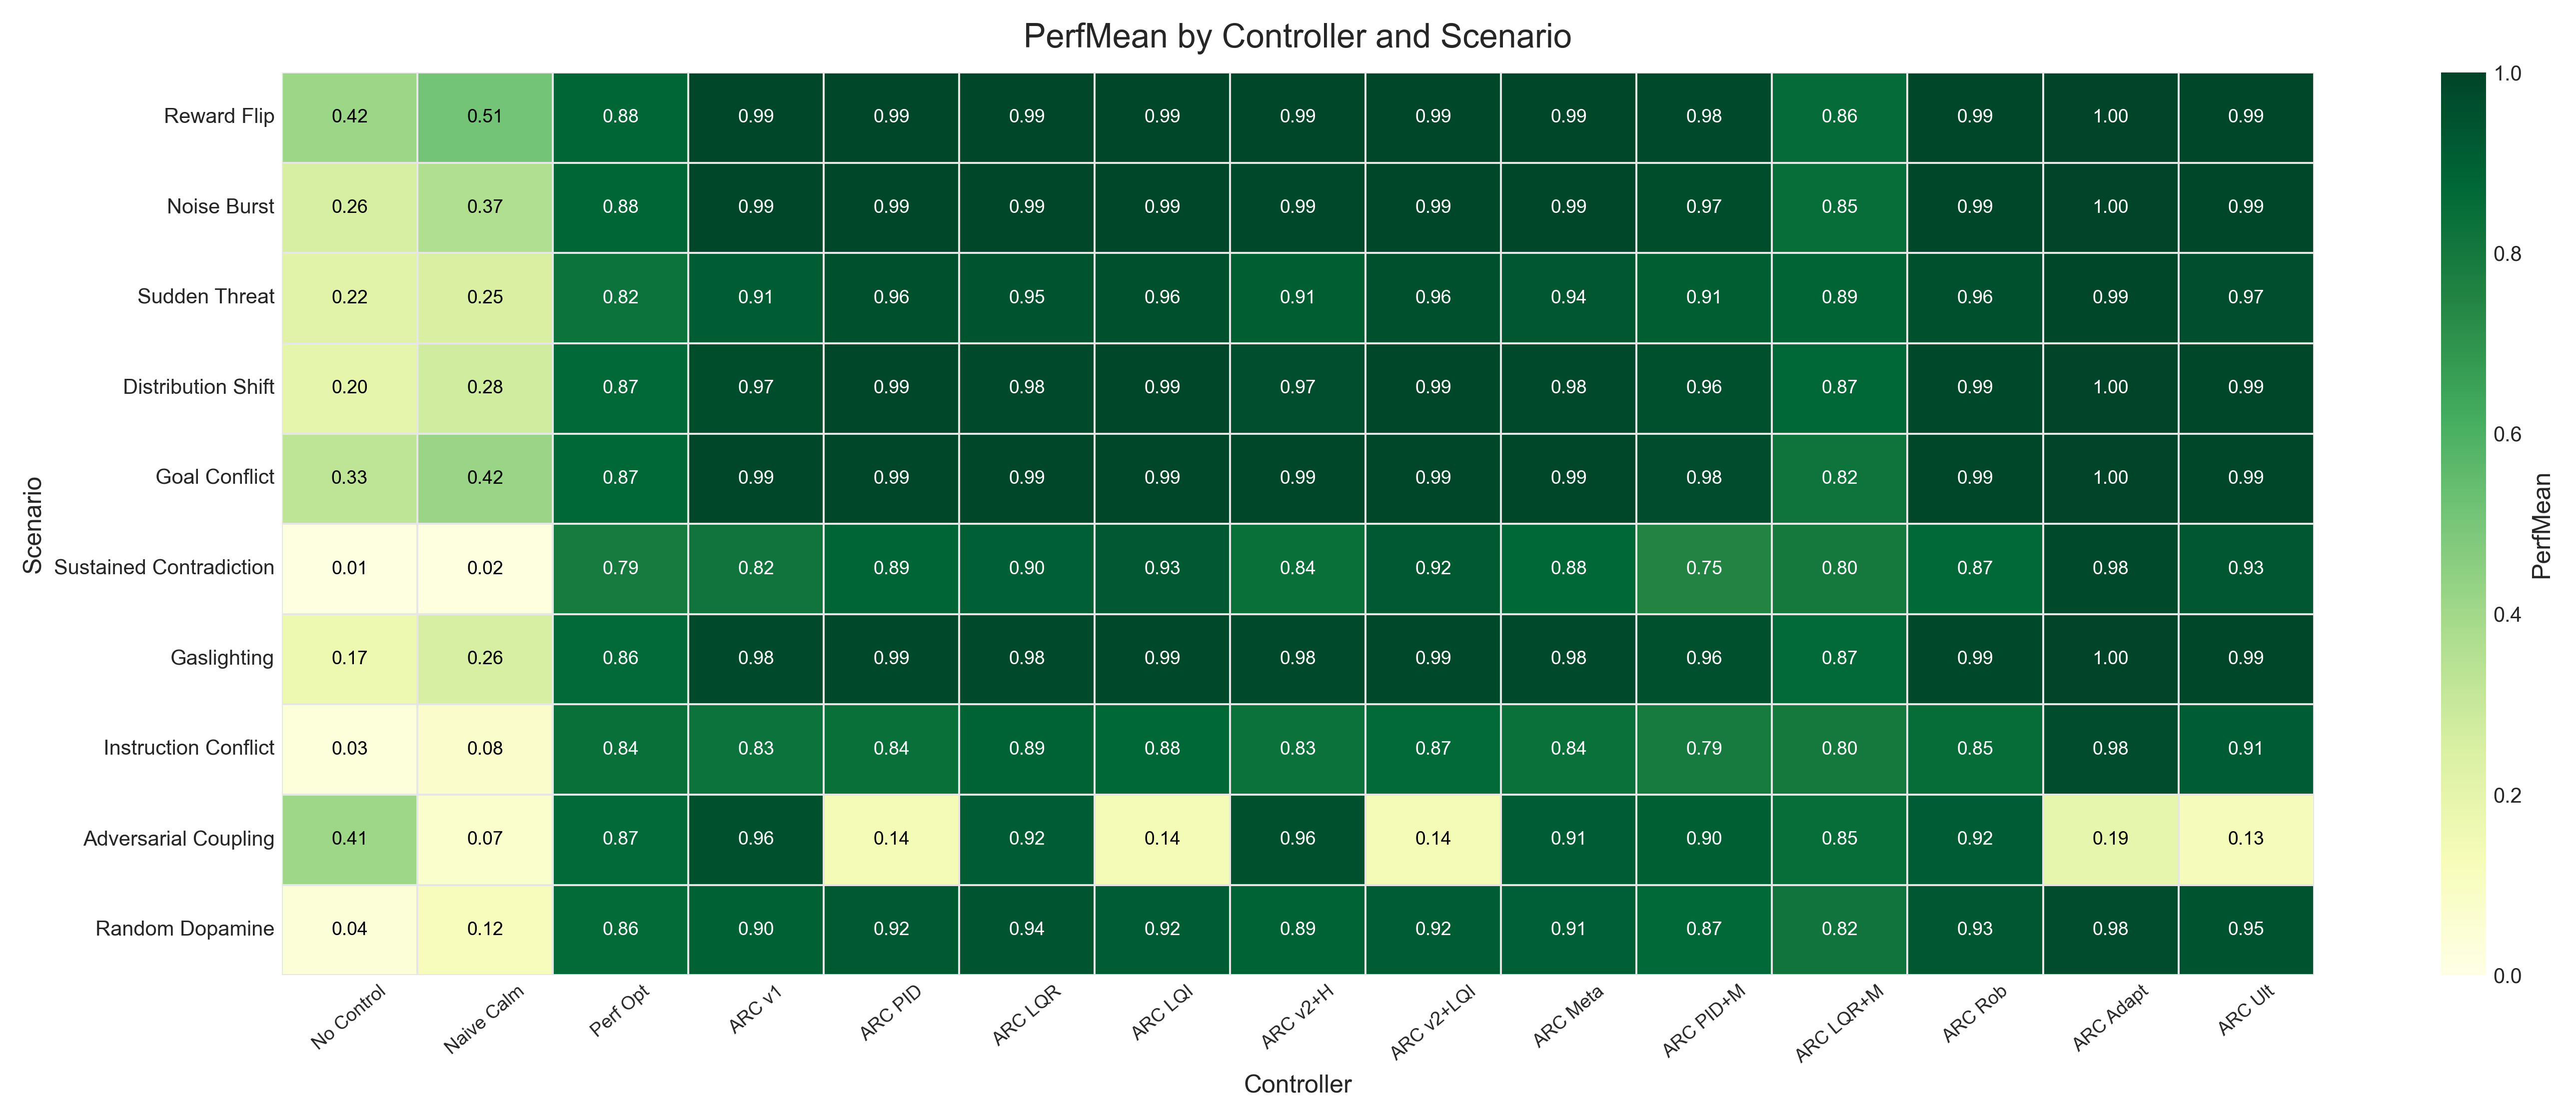
\includegraphics[width=0.96\textwidth]{figures/fig_heatmap_perfmean.png}
    \caption{PerfMean agregado como media sobre 20 semillas para cada par controlador $\times$ escenario. Las filas son las 15 arquitecturas de controlador (de la Tabla~\ref{tab:controller_comparison}); las columnas son los 10 escenarios de simulación ASSB (L1--L3, L5). Mayor (amarillo) es mejor; menor (morado) indica colapso del desempeño. Varios controladores exhiben bandas horizontales casi uniformemente amarillas (\texttt{arc\_robust}, \texttt{arc\_v3\_meta}, \texttt{arc\_v2\_hier}); la celda distintiva clave es la columna derecha (\texttt{adversarial\_coupling}), donde sólo los controladores sin acción integral (o con anti-windup) permanecen brillantes. La uniformidad visual, por lo tanto, necesita ser contrastada con la Tabla~\ref{tab:three_criterion_test} para identificar qué controladores realmente pasan los tres criterios de consistencia. Una banda vertical oscura identifica escenarios que permanecen difíciles para la mayoría de los controladores (p.\ ej.\ \texttt{adversarial\_coupling}). Los valores numéricos por celda están en las Tablas~\ref{tab:g1_reward_flip}--\ref{tab:g11_random_dopamine}.}
    \label{fig:heatmap_perfmean}
\end{figure}

\begin{figure}[htbp]
    \centering
    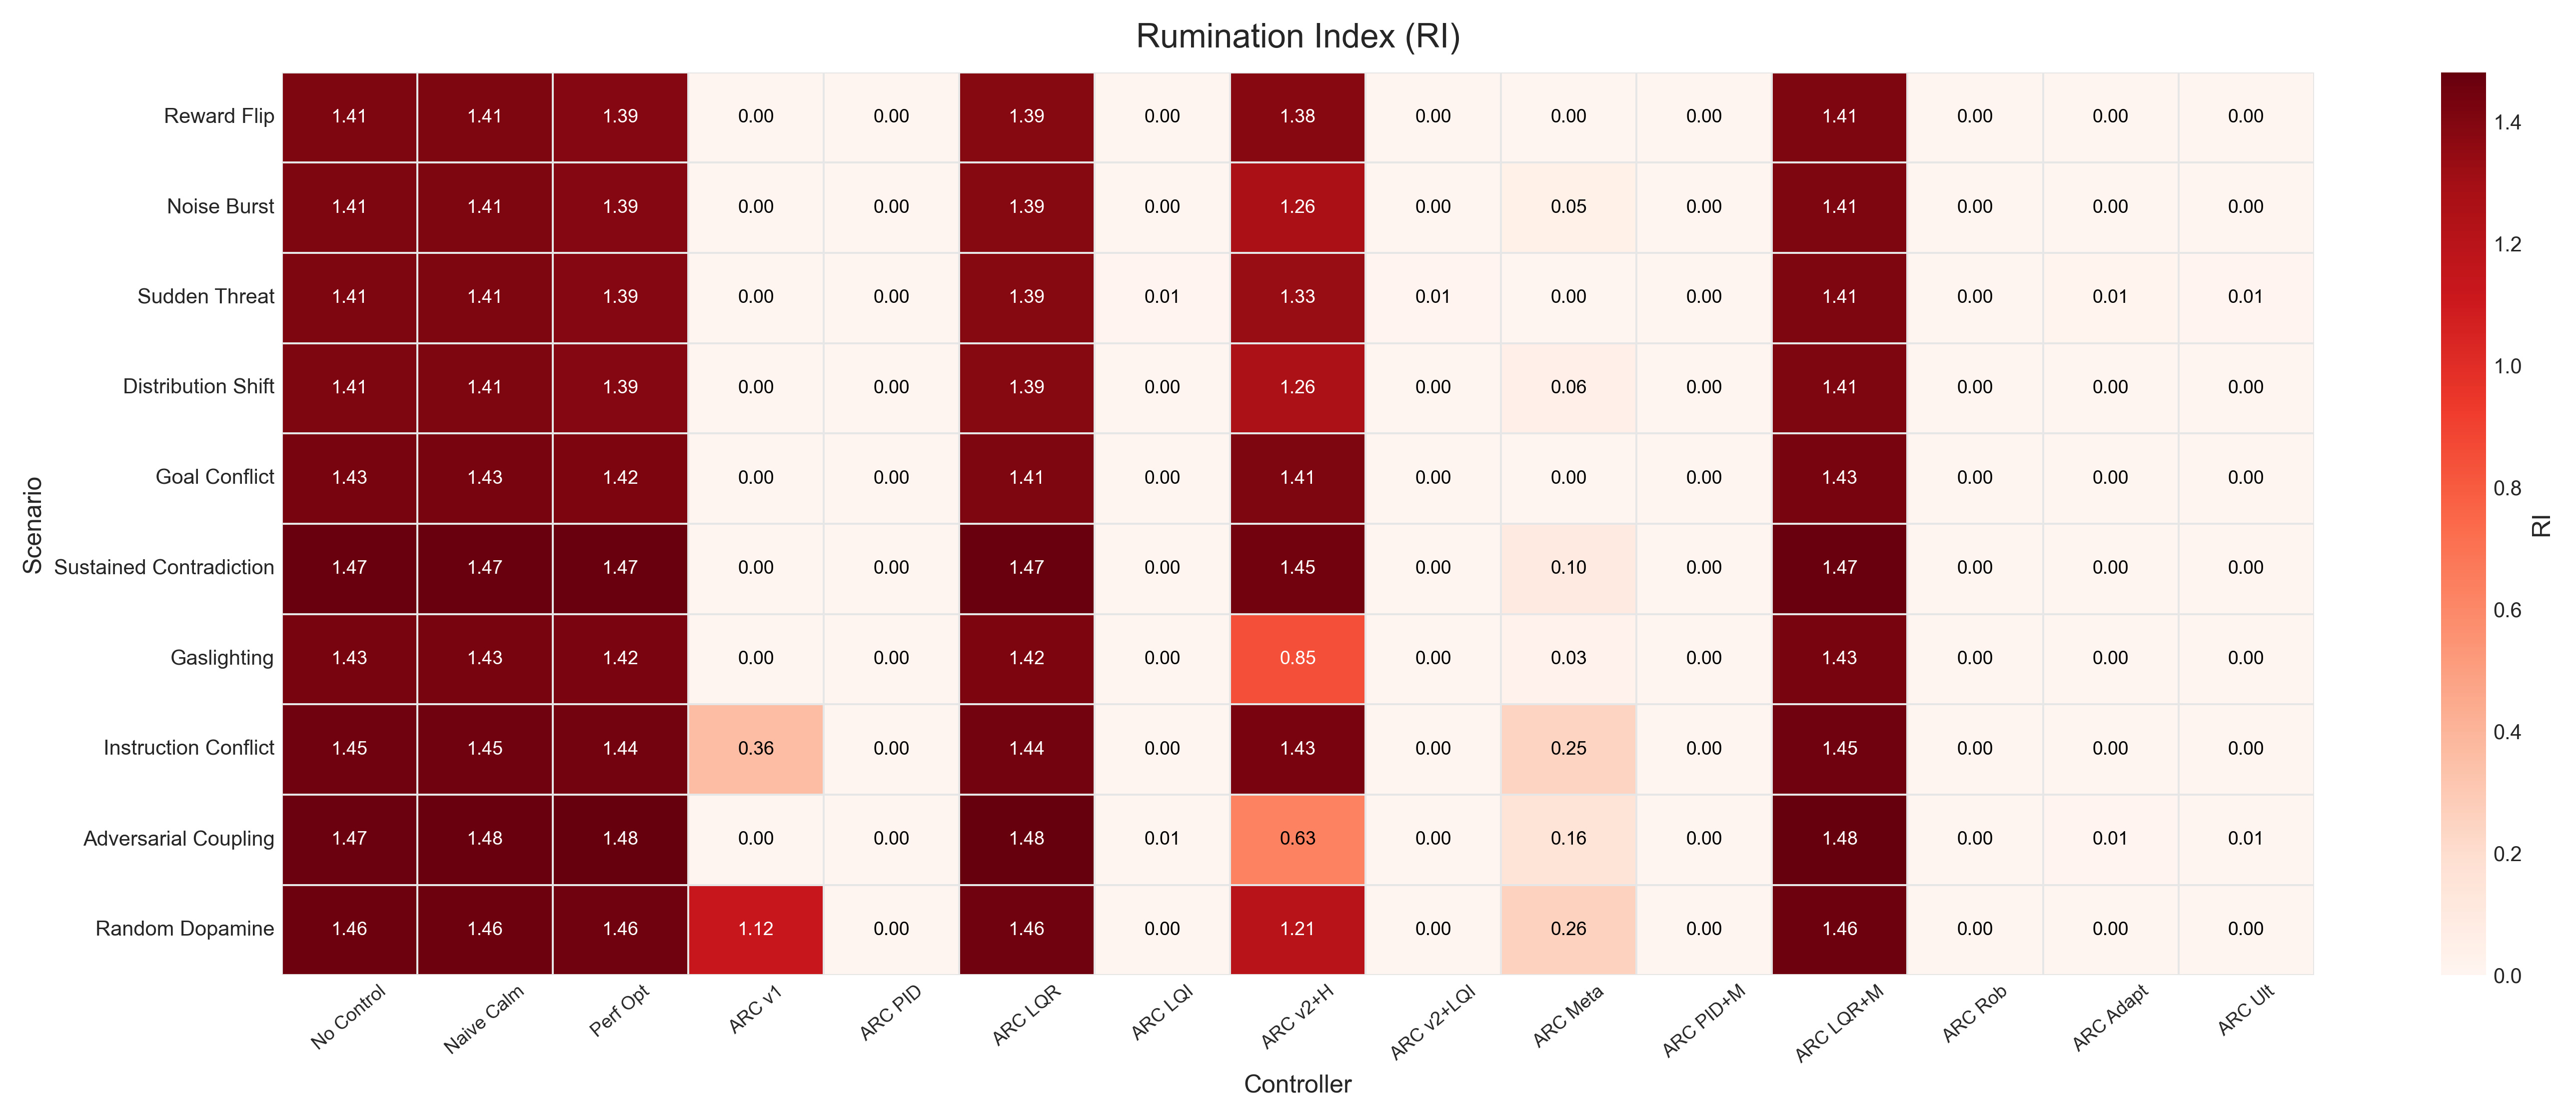
\includegraphics[width=0.96\textwidth]{figures/fig_heatmap_ri.png}
    \caption{Índice de Rumiación agregado como media sobre 20 semillas para cada par controlador $\times$ escenario. Filas / columnas como en la Figura~\ref{fig:heatmap_perfmean}. Menor (morado oscuro $\approx 0$) es mejor; valores $\geq 1$ (amarillo brillante) indican intensidad narrativa sostenida por encima del umbral. Los controladores con acción integral (PID, LQI, MPC+LQI) muestran filas uniformemente oscuras en todas las columnas excepto \texttt{adversarial\_coupling}, donde el windup del integrador produce celdas brillantes. Los valores numéricos por celda están en las Tablas~\ref{tab:g1_reward_flip}--\ref{tab:g11_random_dopamine}.}
\end{figure}

\begin{figure}[htbp]
    \centering
    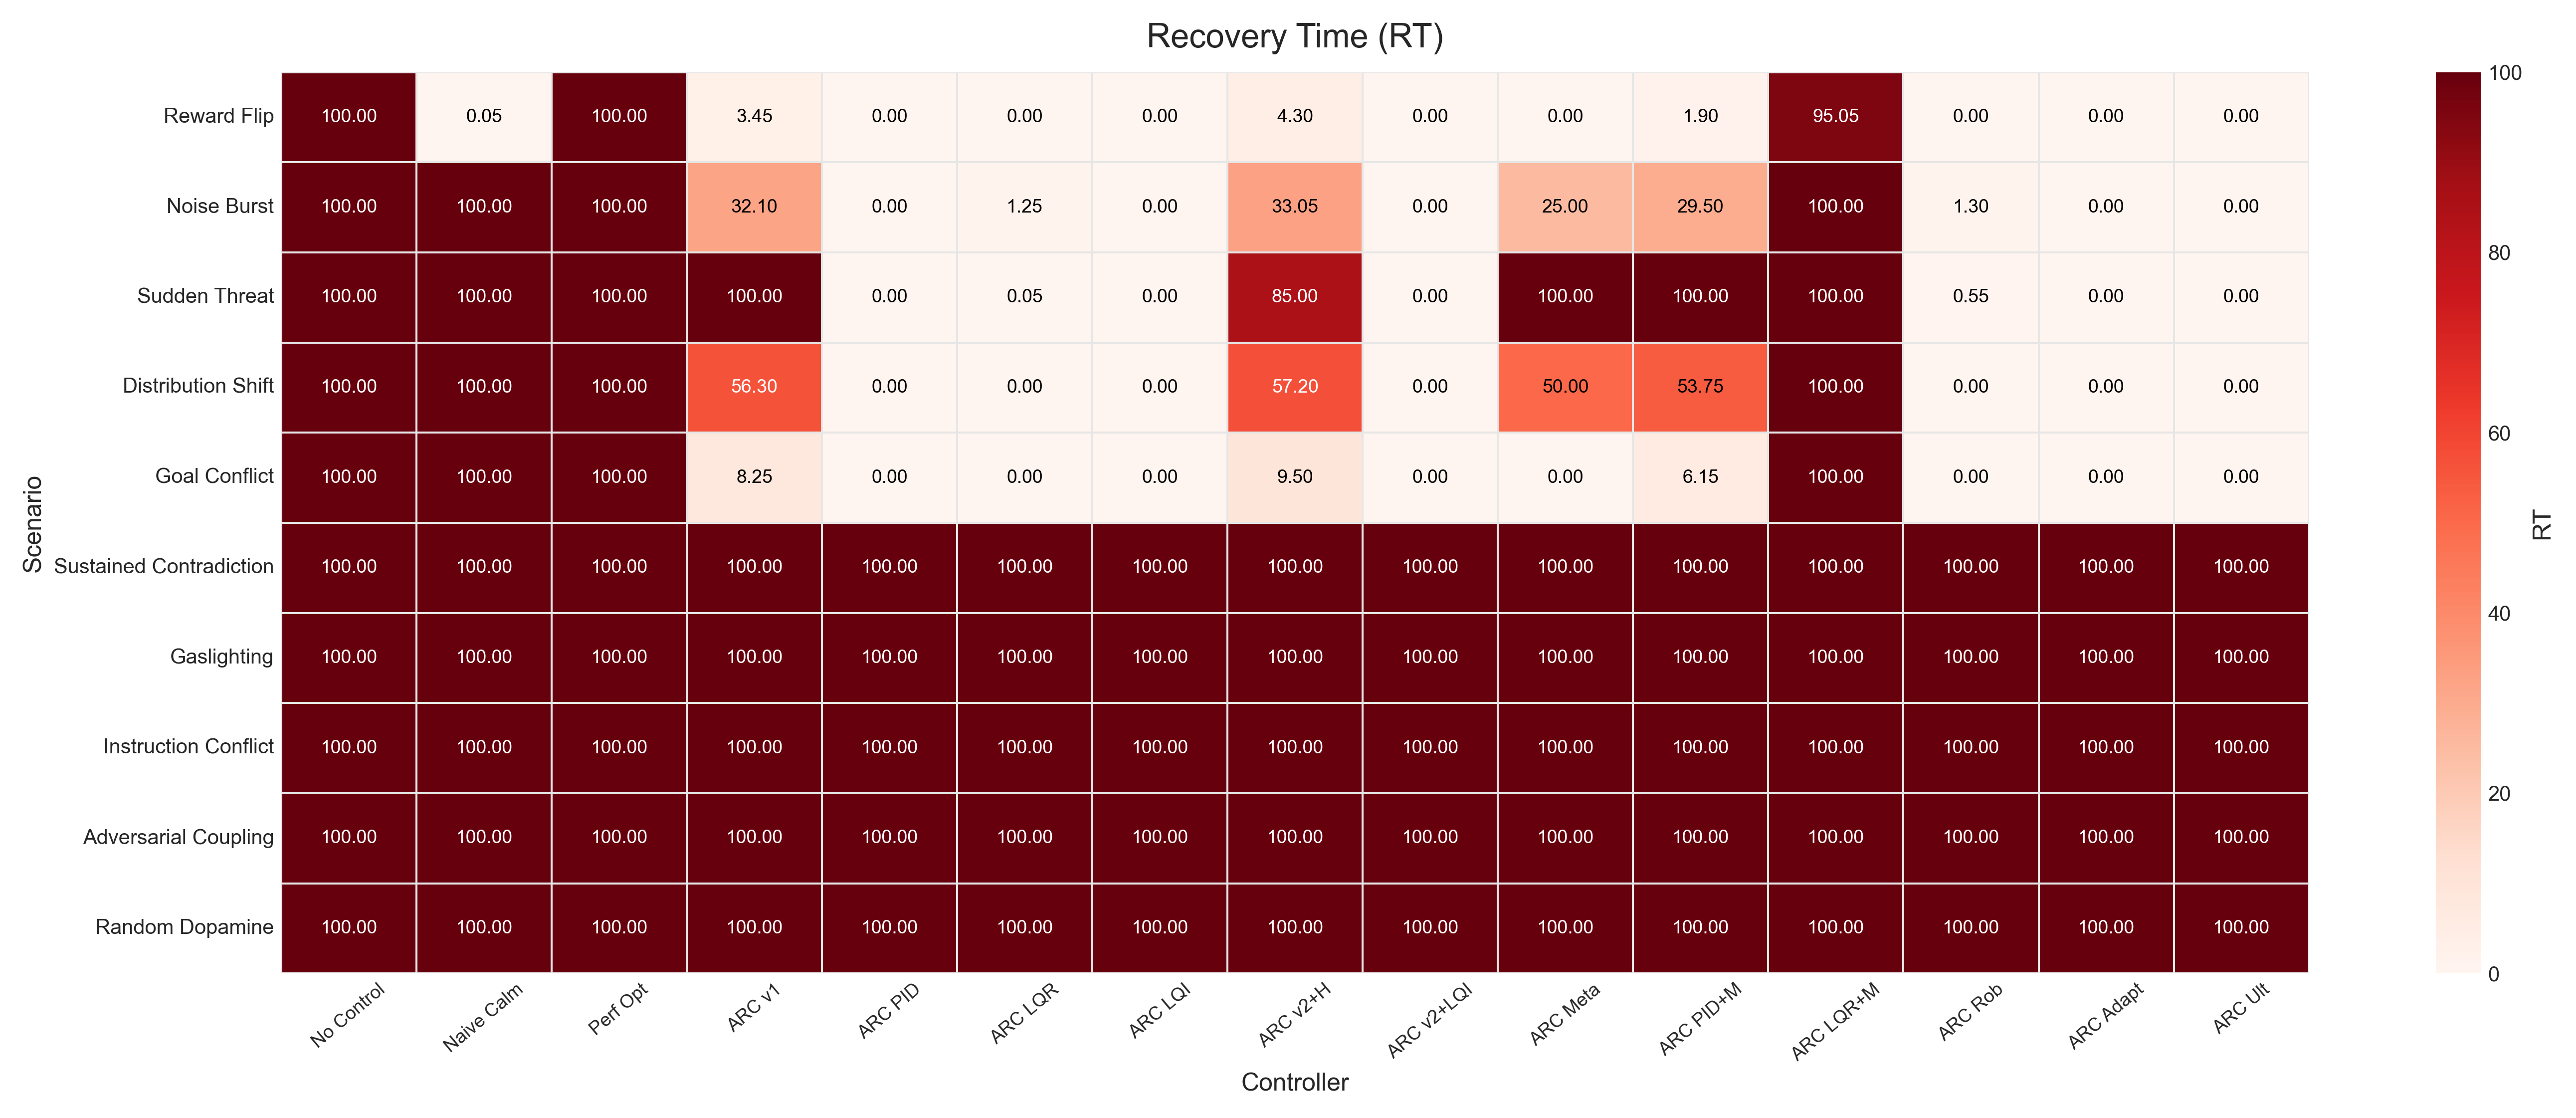
\includegraphics[width=0.96\textwidth]{figures/fig_heatmap_rt.png}
    \caption{Tiempo de Recuperación agregado como media sobre 20 semillas para cada par controlador $\times$ escenario. Filas / columnas como en la Figura~\ref{fig:heatmap_perfmean}. Menor (oscuro) es recuperación más rápida; las celdas saturadas en \texttt{rt\_max} $= 100$ (amarillo brillante) indican que el criterio estricto de recuperación (Apéndice~D.2) no se cumple dentro de la ventana de evaluación para cada semilla. RT está censurado más que indefinido: la banda de valores 100 representa por lo tanto ``sin recuperación detectada bajo el criterio estricto'', no un retardo literal de $100$ pasos. Los valores numéricos por celda están en las Tablas~\ref{tab:g1_reward_flip}--\ref{tab:g11_random_dopamine}.}
\end{figure}

\begin{figure}[htbp]
    \centering
    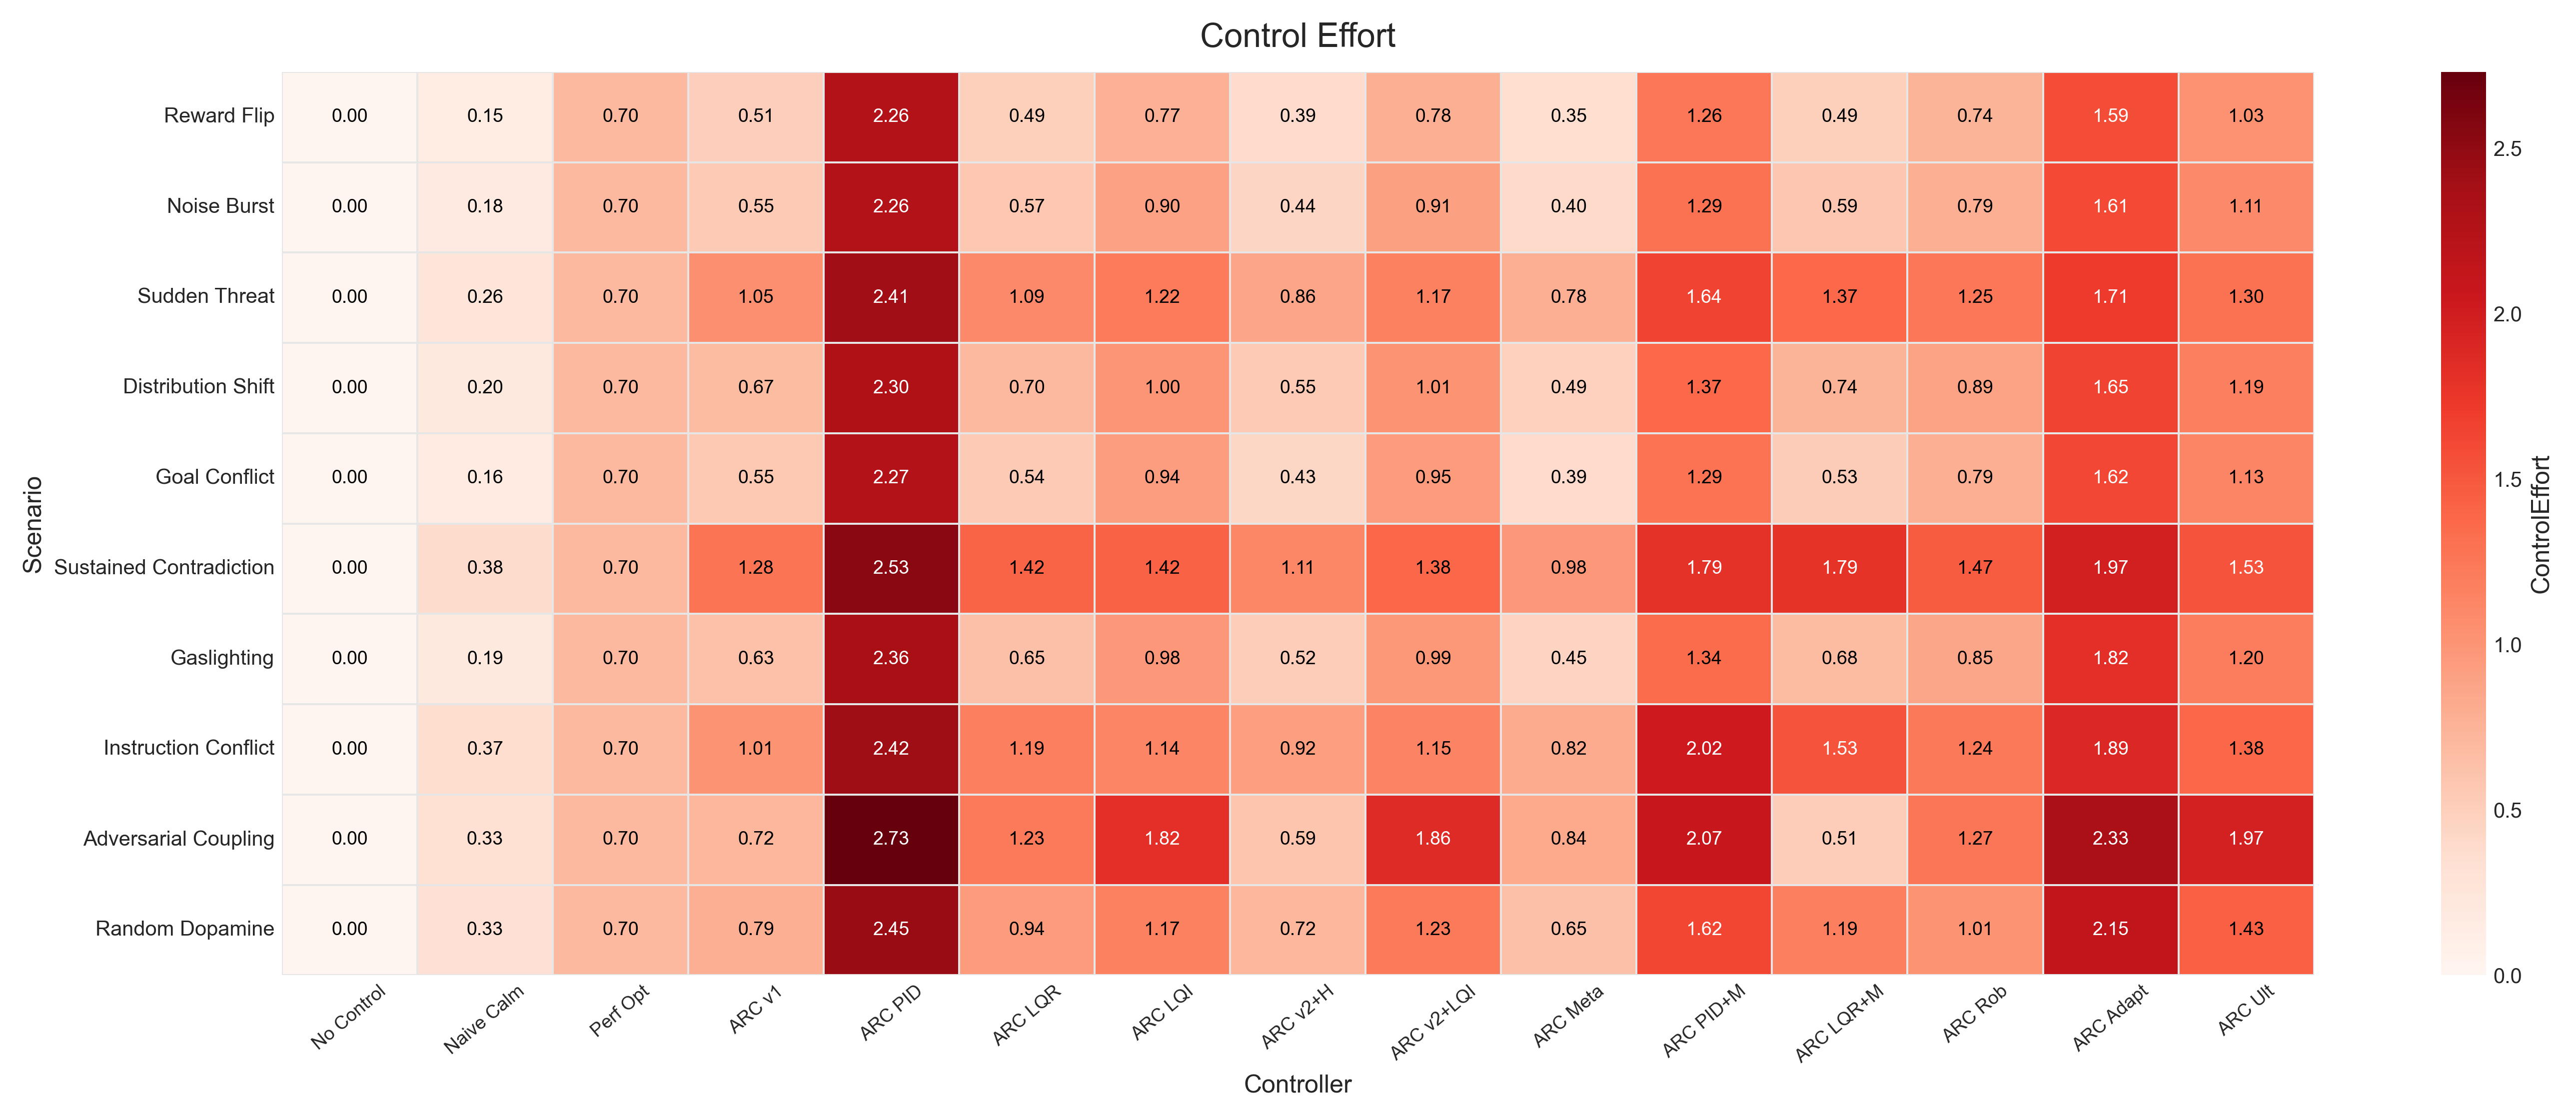
\includegraphics[width=0.96\textwidth]{figures/fig_heatmap_effort.png}
    \caption{ControlEffort agregado como media sobre 20 semillas para cada par controlador $\times$ escenario. Filas / columnas como en la Figura~\ref{fig:heatmap_perfmean}. La escala de color representa la magnitud $\ell_1$ promedio por paso de la acción de control $\mathbf{u}(t)$; menor (oscuro) es más eficiente. La fila del baseline no controlado (\texttt{no\_control}) es uniformemente cero por construcción; los controladores con aumento integral (\texttt{arc\_v1\_pid}, \texttt{arc\_v1\_lqi}, \texttt{arc\_ultimate}) muestran las filas más brillantes, reflejando el mayor esfuerzo requerido para llevar RI a cero. El meta-control (\texttt{arc\_v3\_meta}) alcanza la fila efectiva más oscura entre las variantes ARC. Los valores numéricos por celda están en las Tablas~\ref{tab:g1_reward_flip}--\ref{tab:g11_random_dopamine}.}
\end{figure}

\begin{figure}[htbp]
    \centering
    
\includegraphics[width=0.90\textwidth]{figures/correlation_combined.png}
    \caption{Mapa de calor de correlaciones agregado sobre todas las corridas experimentales (matriz completa $11\times 11$ de métricas ASSB). Los tres pares destacados en la Tabla~\ref{tab:correlations} son un subconjunto pre-registrado y motivado teóricamente; las correlaciones fuertes restantes (p.\ ej.\ Retention--PerfMean, ControlEffort--PerfMean) se discuten como patrones observacionales y no se usan para soportar claims a nivel de hipótesis.}
    \label{fig:correlation_combined}
\end{figure}

\begin{figure}[htbp]
    \centering
    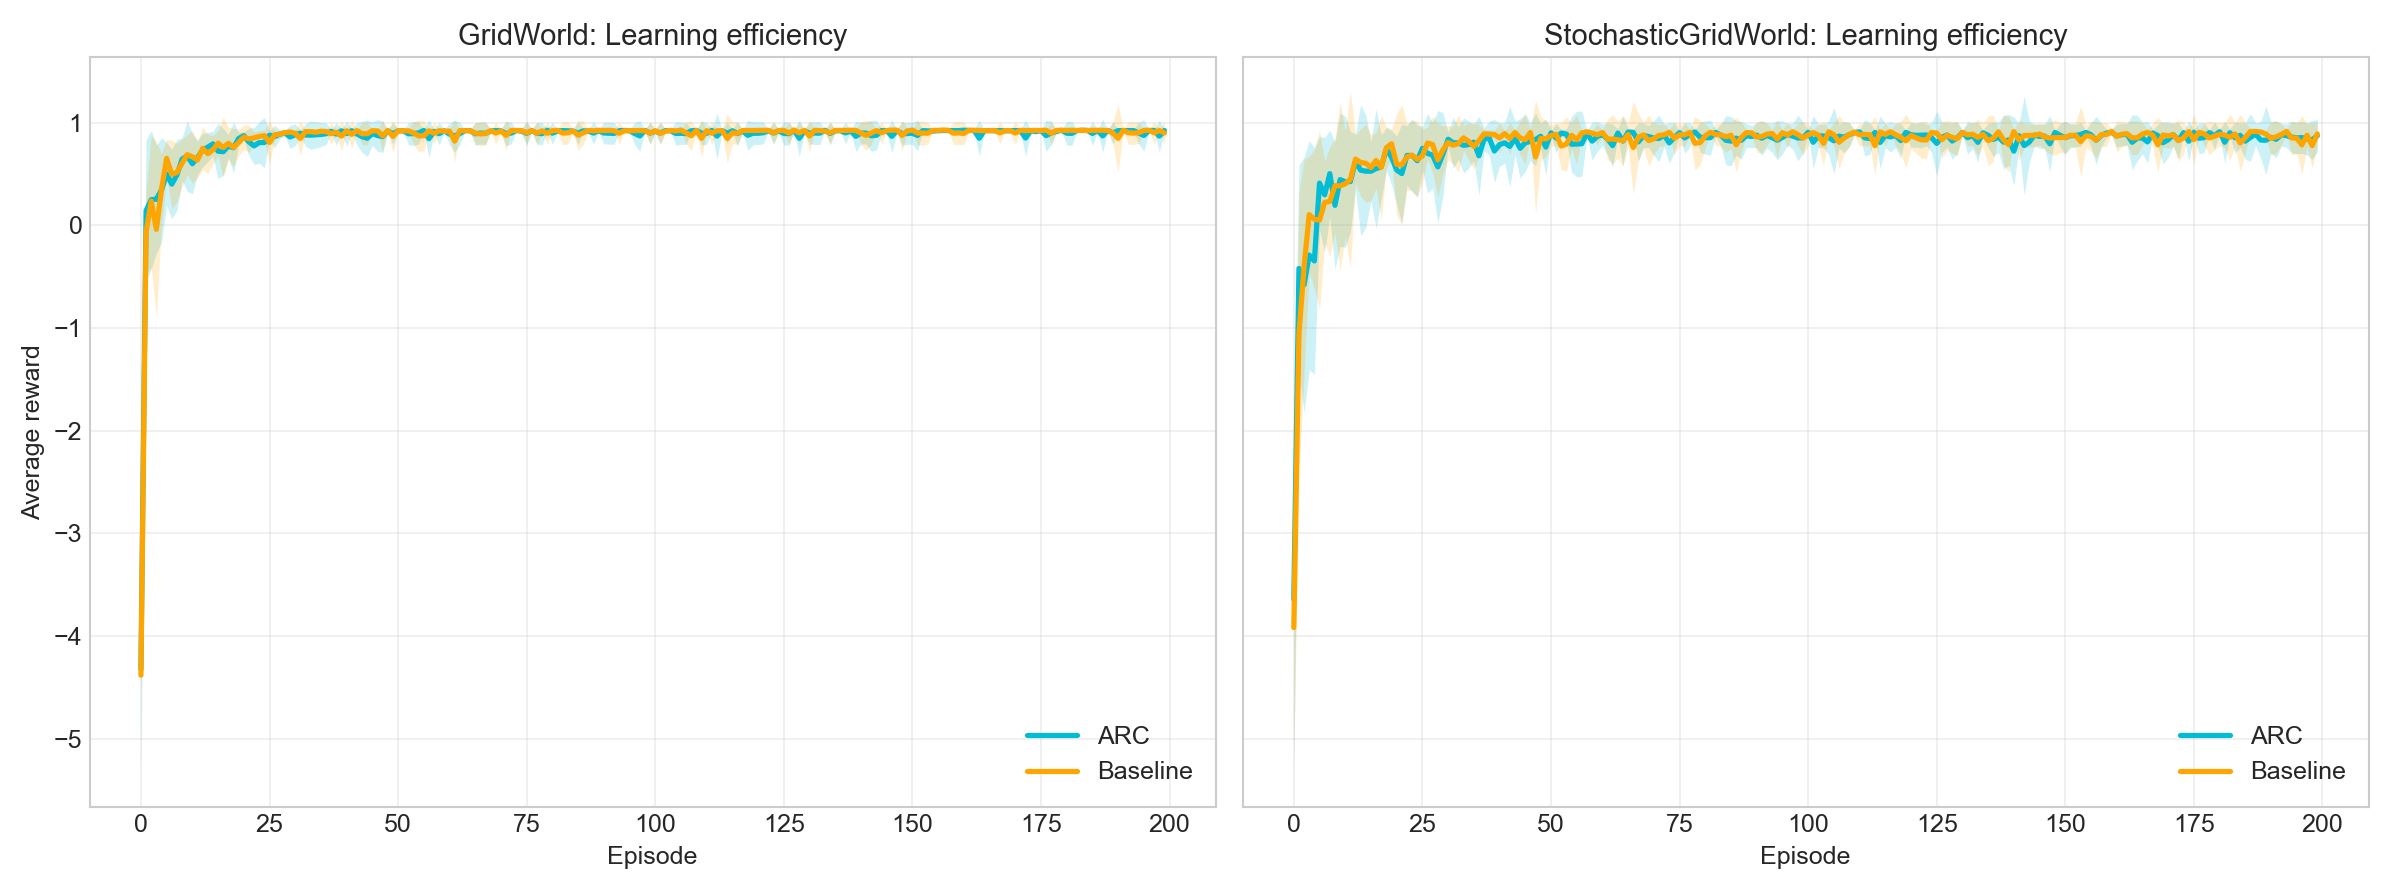
\includegraphics[width=\textwidth]{figures/efficiency_comparison.png}
    \caption{Comparación de eficiencia en GridWorld y StochasticGridWorld. Tanto el agente envuelto por ARC como el baseline alcanzan una tasa de éxito del 100\% en el 20\% final de los episodios (de ahí el segmento plano terminal); las curvas difieren en velocidad del transitorio, con el aprendiz envuelto por ARC cruzando el umbral de éxito móvil del $80\%$ un pequeño número de episodios antes que el baseline en estos entornos saturados. No reclamamos una aceleración significativa aquí --- ambos entornos están en el techo del $100\%$ para ambas condiciones --- y reportamos esto sólo como observación visual. Se requeriría una métrica cuantitativa de tiempo de convergencia (p.\ ej.\ episodios hasta el primer $\geq 95\%$ de éxito móvil) para establecer una diferencia formal; no forma parte del conjunto pre-registrado de métricas ASSB.}
    \label{fig:efficiency}
\end{figure}

\begin{figure}[htbp]
    \centering
    
\includegraphics[width=0.95\textwidth]{figures/sensitivity_scenario.png}
    \caption{Análisis a nivel de escenario (sólo ARC): desempeño, rumiación y tiempo de recuperación varían sustancialmente por tipo de estresor.}
\end{figure}

\begin{figure}[htbp]
    \centering
    
\includegraphics[width=0.95\textwidth]{figures/sensitivity_variance.png}
    \caption{Análisis de varianza entre semillas. Menor varianza indica comportamiento más confiable; los controladores ARC generalmente exhiben distribuciones de desempeño más estrechas que los baselines.}
\end{figure}

\begin{figure}[htbp]
    \centering
    
\includegraphics[width=0.62\textwidth]{figures/correlation_L1.png}
    \caption{Mapa de calor de correlaciones sólo para corridas L1 (línea de estabilidad).}
\end{figure}

\begin{figure}[htbp]
    \centering
    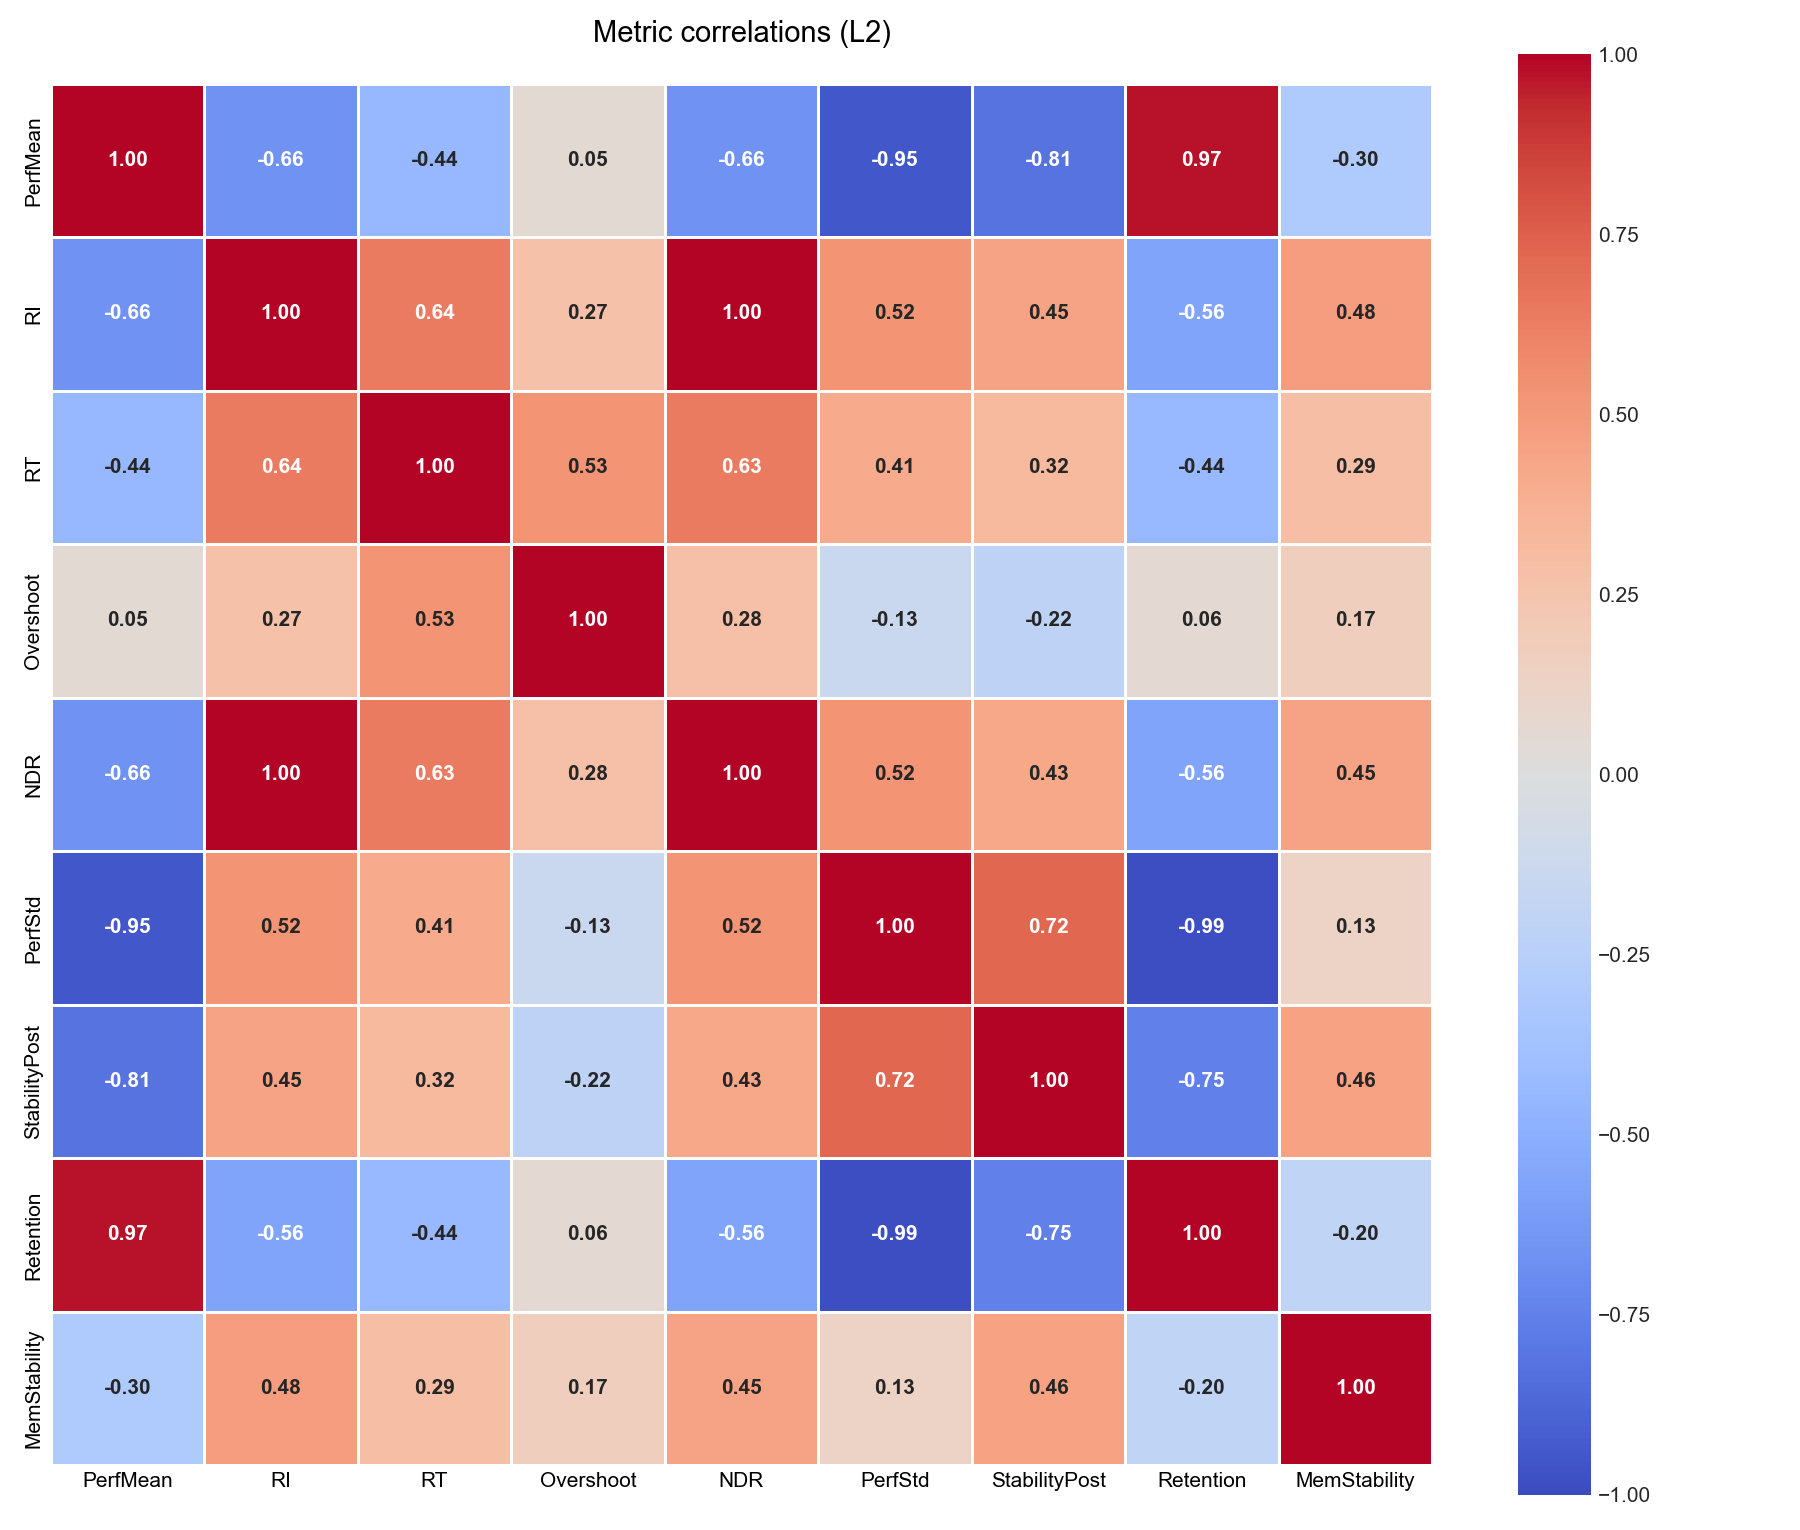
\includegraphics[width=0.62\textwidth]{figures/correlation_L2.png}
    \caption{Mapa de calor de correlaciones sólo para corridas L2 (línea de memoria y aprendizaje continuo).}
\end{figure}

\begin{figure}[htbp]
    \centering
    
\includegraphics[width=0.62\textwidth]{figures/correlation_L3.png}
    \caption{Mapa de calor de correlaciones sólo para corridas L3 (línea de pruebas de estrés anti-rumiación).}
\end{figure}

\begin{figure}[htbp]
    \centering
    
\includegraphics[width=0.62\textwidth]{figures/correlation_L4.png}
    \caption{Mapa de calor de correlaciones sólo para corridas L4 (línea de eficiencia del meta-control).}
\end{figure}

\begin{figure}[htbp]
    \centering
    
\includegraphics[width=0.62\textwidth]{figures/correlation_L4_meta.png}
    \caption{Mapa de calor de correlaciones para corridas enfocadas en meta-control (L4\_meta).}
\end{figure}

\begin{figure}[htbp]
    \centering
    
\includegraphics[width=0.62\textwidth]{figures/correlation_L5.png}
    \caption{Mapa de calor de correlaciones sólo para corridas L5 (línea de seguridad adversarial).}
\end{figure}

\FloatBarrier
\section{Parámetros de Configuración}

\begin{table}[htbp]
\centering
\caption{Parámetros de Configuración (de \texttt{configs/v2.yaml})}
\label{tab:config}
\begin{tabular}{@{}lcl@{}}
\toprule
Parámetro & Valor & Descripción \\ \midrule
a\_safe & 0.60 & Umbral seguro de arousal \\
s\_safe & 0.55 & Umbral seguro de intensidad narrativa \\
s\_rum\_tau & 0.55 & Umbral de rumiación \\
arc\_w\_u & 0.40 & Peso de incertidumbre en el riesgo \\
arc\_w\_a & 0.40 & Peso de arousal en el riesgo \\
arc\_w\_s & 0.35 & Peso de narrativa en el riesgo \\
arc\_k\_dmg & 0.95 & Ganancia de supresión DMN \\
arc\_k\_calm & 0.85 & Ganancia de calma \\
arc\_k\_att & 0.75 & Ganancia de impulso atencional \\
horizon & 160 & Longitud del episodio (simulación) \\
shock\_t & 60 & Tiempo de inicio de la perturbación \\ \bottomrule
\end{tabular}
\end{table}

\section{Resultados Detallados del Benchmark}
Este apéndice provee resultados a nivel de escenario para las 15 arquitecturas de controlador a lo largo de los escenarios validados (media sobre 20 semillas por escenario salvo indicación en contrario). Reportamos PerfMean, Índice de Rumiación (RI), Ratio de Dominancia Narrativa (NDR), Tiempo de Recuperación (RT; saturado en \texttt{rt\_max}, donde RT = \texttt{rt\_max} indica sin recuperación bajo el criterio estricto dentro de la ventana de evaluación) y ControlEffort.

\subsection{Línea 1: Estabilidad (Shocks de Valor e Incertidumbre)}

\scenarioheader{Reward Flip}

\begin{table}[H]
\centering
\footnotesize
\caption{Resultados detallados para L1 / \texttt{reward\_flip} (media sobre 20 semillas).}
\label{tab:g1_reward_flip}
\begin{adjustbox}{max width=\textwidth}
\begin{tabular}{@{}lcccc@{}}
\toprule
Controlador & PerfMean & RI & RT & ControlEffort \\ \midrule
arc\_adaptive & 0.998 & 0.000 & 0.000 & 1.587 \\
arc\_ultimate & 0.995 & 0.000 & 0.000 & 1.027 \\
arc\_v2\_hier & 0.994 & 1.377 & 4.300 & 0.390 \\
arc\_v1\_lqr & 0.994 & 1.386 & 0.000 & 0.494 \\
arc\_v1 & 0.994 & 0.000 & 3.450 & 0.508 \\
arc\_robust & 0.994 & 0.000 & 0.000 & 0.744 \\
arc\_v3\_meta & 0.993 & 0.000 & 0.000 & 0.353 \\
arc\_v1\_lqi & 0.991 & 0.000 & 0.000 & 0.773 \\
arc\_v2\_lqi & 0.991 & 0.000 & 0.000 & 0.784 \\
arc\_v1\_pid & 0.991 & 0.000 & 0.000 & 2.257 \\
arc\_v3\_pid\_meta & 0.978 & 0.000 & 1.900 & 1.257 \\
perf\_optimized & 0.880 & 1.394 & 100.000 & 0.700 \\
arc\_v3\_lqr\_meta & 0.859 & 1.407 & 95.050 & 0.492 \\
naive\_calm & 0.508 & 1.408 & 0.050 & 0.149 \\
no\_control & 0.415 & 1.408 & 100.000 & 0.000 \\ \bottomrule
\end{tabular}
\end{adjustbox}
\end{table}

\scenarioheader{Noise Burst}

\begin{table}[H]
\centering
\footnotesize
\caption{Resultados detallados para L1 / \texttt{noise\_burst} (media sobre 20 semillas).}
\label{tab:g2_noise_burst}
\begin{adjustbox}{max width=\textwidth}
\begin{tabular}{@{}lcccc@{}}
\toprule
Controlador & PerfMean & RI & RT & ControlEffort \\ \midrule
arc\_adaptive & 0.998 & 0.000 & 0.000 & 1.605 \\
arc\_ultimate & 0.995 & 0.000 & 0.000 & 1.106 \\
arc\_robust & 0.993 & 0.000 & 1.300 & 0.785 \\
arc\_v3\_meta & 0.993 & 0.051 & 25.000 & 0.399 \\
arc\_v1\_lqr & 0.993 & 1.386 & 1.250 & 0.566 \\
arc\_v1\_lqi & 0.991 & 0.000 & 0.000 & 0.905 \\
arc\_v2\_lqi & 0.991 & 0.000 & 0.000 & 0.915 \\
arc\_v1\_pid & 0.991 & 0.000 & 0.000 & 2.257 \\
arc\_v1 & 0.989 & 0.000 & 32.100 & 0.550 \\
arc\_v2\_hier & 0.987 & 1.263 & 33.050 & 0.444 \\
arc\_v3\_pid\_meta & 0.972 & 0.000 & 29.500 & 1.290 \\
perf\_optimized & 0.880 & 1.394 & 100.000 & 0.700 \\
arc\_v3\_lqr\_meta & 0.848 & 1.407 & 100.000 & 0.585 \\
naive\_calm & 0.365 & 1.408 & 100.000 & 0.177 \\
no\_control & 0.259 & 1.408 & 100.000 & 0.000 \\ \bottomrule
\end{tabular}
\end{adjustbox}
\end{table}

\scenarioheader{Sudden Threat}

\begin{table}[H]
\centering
\footnotesize
\caption{Resultados detallados para L1 / \texttt{sudden\_threat} (media sobre 20 semillas).}
\label{tab:g3_sudden_threat}
\begin{adjustbox}{max width=\textwidth}
\begin{tabular}{@{}lcccc@{}}
\toprule
Controlador & PerfMean & RI & RT & ControlEffort \\ \midrule
arc\_adaptive & 0.989 & 0.013 & 0.000 & 1.707 \\
arc\_ultimate & 0.968 & 0.010 & 0.000 & 1.298 \\
arc\_v1\_pid & 0.964 & 0.000 & 0.000 & 2.410 \\
arc\_v1\_lqi & 0.964 & 0.008 & 0.000 & 1.222 \\
arc\_v2\_lqi & 0.963 & 0.008 & 0.000 & 1.173 \\
arc\_robust & 0.959 & 0.005 & 0.550 & 1.252 \\
arc\_v1\_lqr & 0.949 & 1.386 & 0.050 & 1.088 \\
arc\_v3\_meta & 0.936 & 0.000 & 100.000 & 0.783 \\
arc\_v1 & 0.914 & 0.000 & 100.000 & 1.054 \\
arc\_v3\_pid\_meta & 0.908 & 0.000 & 100.000 & 1.643 \\
arc\_v2\_hier & 0.907 & 1.333 & 85.000 & 0.864 \\
arc\_v3\_lqr\_meta & 0.890 & 1.407 & 100.000 & 1.370 \\
perf\_optimized & 0.825 & 1.394 & 100.000 & 0.700 \\
naive\_calm & 0.252 & 1.408 & 100.000 & 0.262 \\
no\_control & 0.217 & 1.408 & 100.000 & 0.000 \\ \bottomrule
\end{tabular}
\end{adjustbox}
\end{table}

\FloatBarrier
\subsection{Línea 2: Memoria y Aprendizaje Continuo}

\scenarioheader{Distribution Shift}

\begin{table}[H]
\centering
\footnotesize
\caption{Resultados detallados para L2 / \texttt{distribution\_shift} (media sobre 20 semillas).}
\label{tab:g4_distribution_shift}
\begin{adjustbox}{max width=\textwidth}
\begin{tabular}{@{}lcccc@{}}
\toprule
Controlador & PerfMean & Retention & RI & ControlEffort \\ \midrule
arc\_adaptive & 0.998 & 1.000 & 0.000 & 1.645 \\
arc\_ultimate & 0.995 & 1.000 & 0.000 & 1.186 \\
arc\_v1\_lqi & 0.991 & 1.000 & 0.000 & 0.999 \\
arc\_v2\_lqi & 0.991 & 1.000 & 0.000 & 1.008 \\
arc\_v1\_pid & 0.991 & 1.000 & 0.000 & 2.296 \\
arc\_robust & 0.985 & 1.000 & 0.000 & 0.892 \\
arc\_v1\_lqr & 0.984 & 1.000 & 1.386 & 0.695 \\
arc\_v3\_meta & 0.982 & 1.000 & 0.057 & 0.486 \\
arc\_v1 & 0.972 & 1.000 & 0.000 & 0.674 \\
arc\_v2\_hier & 0.968 & 1.000 & 1.258 & 0.548 \\
arc\_v3\_pid\_meta & 0.959 & 1.000 & 0.000 & 1.372 \\
arc\_v3\_lqr\_meta & 0.871 & 0.989 & 1.407 & 0.739 \\
perf\_optimized & 0.869 & 0.943 & 1.394 & 0.700 \\
naive\_calm & 0.276 & 0.155 & 1.408 & 0.200 \\
no\_control & 0.199 & 0.000 & 1.408 & 0.000 \\ \bottomrule
\end{tabular}
\end{adjustbox}
\end{table}

\scenarioheader{Goal Conflict}

\begin{table}[H]
\centering
\footnotesize
\caption{Resultados detallados para L2 / \texttt{goal\_conflict} (media sobre 20 semillas).}
\label{tab:g5_goal_conflict}
\begin{adjustbox}{max width=\textwidth}
\begin{tabular}{@{}lcccc@{}}
\toprule
Controlador & PerfMean & Retention & RI & ControlEffort \\ \midrule
arc\_adaptive & 0.997 & 1.000 & 0.000 & 1.620 \\
arc\_ultimate & 0.993 & 1.000 & 0.000 & 1.134 \\
arc\_v1\_lqr & 0.993 & 1.000 & 1.408 & 0.544 \\
arc\_robust & 0.992 & 1.000 & 0.000 & 0.785 \\
arc\_v3\_meta & 0.991 & 1.000 & 0.000 & 0.388 \\
arc\_v1\_lqi & 0.991 & 1.000 & 0.000 & 0.938 \\
arc\_v2\_lqi & 0.991 & 1.000 & 0.000 & 0.947 \\
arc\_v1 & 0.990 & 1.000 & 0.000 & 0.555 \\
arc\_v1\_pid & 0.990 & 1.000 & 0.000 & 2.270 \\
arc\_v2\_hier & 0.989 & 1.000 & 1.410 & 0.430 \\
arc\_v3\_pid\_meta & 0.976 & 1.000 & 0.000 & 1.289 \\
perf\_optimized & 0.873 & 0.957 & 1.417 & 0.700 \\
arc\_v3\_lqr\_meta & 0.822 & 0.980 & 1.434 & 0.529 \\
naive\_calm & 0.420 & 0.452 & 1.434 & 0.162 \\
no\_control & 0.326 & 0.344 & 1.434 & 0.000 \\ \bottomrule
\end{tabular}
\end{adjustbox}
\end{table}

\FloatBarrier
\subsection{Línea 3: Anti-Rumiación (Bucles Narrativos)}

\scenarioheader{Sustained Contradiction}

\begin{table}[H]
\centering
\footnotesize
\caption{Resultados detallados para L3 / \texttt{sustained\_contradiction} (media sobre 20 semillas).}
\label{tab:g6_sustained_contradiction}
\begin{adjustbox}{max width=\textwidth}
\begin{tabular}{@{}lcccc@{}}
\toprule
Controlador & PerfMean & RI & NDR & ControlEffort \\ \midrule
arc\_adaptive & 0.981 & 0.003 & 0.000 & 1.974 \\
arc\_ultimate & 0.934 & 0.000 & 0.000 & 1.534 \\
arc\_v1\_lqi & 0.929 & 0.000 & 0.000 & 1.420 \\
arc\_v2\_lqi & 0.922 & 0.000 & 0.000 & 1.384 \\
arc\_v1\_lqr & 0.904 & 1.472 & 0.881 & 1.417 \\
arc\_v1\_pid & 0.886 & 0.000 & 0.000 & 2.531 \\
arc\_v3\_meta & 0.879 & 0.101 & 0.000 & 0.979 \\
arc\_robust & 0.868 & 0.000 & 0.000 & 1.465 \\
arc\_v2\_hier & 0.837 & 1.449 & 0.821 & 1.112 \\
arc\_v1 & 0.817 & 0.000 & 0.000 & 1.278 \\
arc\_v3\_lqr\_meta & 0.801 & 1.472 & 0.842 & 1.790 \\
perf\_optimized & 0.790 & 1.472 & 0.957 & 0.700 \\
arc\_v3\_pid\_meta & 0.753 & 0.000 & 0.000 & 1.793 \\
naive\_calm & 0.018 & 1.472 & 0.987 & 0.380 \\
no\_control & 0.014 & 1.472 & 0.987 & 0.000 \\ \bottomrule
\end{tabular}
\end{adjustbox}
\end{table}

\scenarioheader{Gaslighting}

\begin{table}[H]
\centering
\footnotesize
\caption{Resultados detallados para L3 / \texttt{gaslighting} (media sobre 20 semillas).}
\label{tab:g7_gaslighting}
\begin{adjustbox}{max width=\textwidth}
\begin{tabular}{@{}lcccc@{}}
\toprule
Controlador & PerfMean & RI & NDR & ControlEffort \\ \midrule
arc\_adaptive & 0.998 & 0.000 & 0.000 & 1.816 \\
arc\_ultimate & 0.992 & 0.000 & 0.000 & 1.196 \\
arc\_v1\_lqi & 0.988 & 0.000 & 0.000 & 0.977 \\
arc\_v2\_lqi & 0.988 & 0.000 & 0.000 & 0.986 \\
arc\_v1\_pid & 0.987 & 0.000 & 0.000 & 2.357 \\
arc\_robust & 0.985 & 0.000 & 0.000 & 0.854 \\
arc\_v1\_lqr & 0.983 & 1.417 & 0.810 & 0.649 \\
arc\_v3\_meta & 0.982 & 0.027 & 0.000 & 0.453 \\
arc\_v1 & 0.980 & 0.000 & 0.000 & 0.634 \\
arc\_v2\_hier & 0.978 & 0.848 & 0.521 & 0.515 \\
arc\_v3\_pid\_meta & 0.962 & 0.000 & 0.000 & 1.344 \\
arc\_v3\_lqr\_meta & 0.865 & 1.430 & 0.745 & 0.677 \\
perf\_optimized & 0.865 & 1.422 & 0.814 & 0.700 \\
naive\_calm & 0.258 & 1.431 & 0.818 & 0.194 \\
no\_control & 0.171 & 1.431 & 0.877 & 0.000 \\ \bottomrule
\end{tabular}
\end{adjustbox}
\end{table}

\scenarioheader{Instruction Conflict}

\begin{table}[H]
\centering
\footnotesize
\caption{Resultados detallados para L3 / \texttt{instruction\_conflict} (media sobre 20 semillas).}
\label{tab:g8_instruction_conflict}
\begin{adjustbox}{max width=\textwidth}
\begin{tabular}{@{}lcccc@{}}
\toprule
Controlador & PerfMean & RI & NDR & ControlEffort \\ \midrule
arc\_adaptive & 0.976 & 0.000 & 0.000 & 1.892 \\
arc\_ultimate & 0.912 & 0.000 & 0.000 & 1.380 \\
arc\_v1\_lqr & 0.894 & 1.444 & 0.697 & 1.192 \\
arc\_v1\_lqi & 0.877 & 0.000 & 0.000 & 1.140 \\
arc\_v2\_lqi & 0.866 & 0.000 & 0.000 & 1.146 \\
arc\_robust & 0.854 & 0.000 & 0.000 & 1.242 \\
perf\_optimized & 0.839 & 1.445 & 0.964 & 0.700 \\
arc\_v1\_pid & 0.839 & 0.000 & 0.000 & 2.415 \\
arc\_v3\_meta & 0.835 & 0.248 & 0.000 & 0.820 \\
arc\_v2\_hier & 0.830 & 1.429 & 0.663 & 0.919 \\
arc\_v1 & 0.826 & 0.359 & 0.000 & 1.010 \\
arc\_v3\_lqr\_meta & 0.798 & 1.453 & 0.676 & 1.535 \\
arc\_v3\_pid\_meta & 0.792 & 0.000 & 0.000 & 2.020 \\
naive\_calm & 0.076 & 1.453 & 0.694 & 0.369 \\
no\_control & 0.034 & 1.453 & 0.969 & 0.000 \\ \bottomrule
\end{tabular}
\end{adjustbox}
\end{table}

\FloatBarrier
\subsection{Línea 4: Eficiencia del Meta-Control}

El meta-control se evalúa como análisis transversal sobre la suite completa de 10 escenarios de simulación (L1-L3 y L5; 20 semillas cada uno).

\begin{table}[H]
\centering
\footnotesize
\caption{Comparación de eficiencia del meta-control agregada sobre la suite de simulación completa (10 escenarios $\times$ 20 semillas).}
\label{tab:g9_meta_control}
\begin{tabular}{@{}lccc@{}}
\toprule
Controlador & PerfMean & RI & ControlEffort \\ \midrule
arc\_v3\_meta & 0.941 & 0.090 & 0.615 \\
arc\_v1 & 0.934 & 0.148 & 0.777 \\ \bottomrule
\end{tabular}
\end{table}

\FloatBarrier
\clearpage
\subsection{Línea 5: Seguridad Adversarial}

\scenarioheader{Adversarial Coupling}

\begin{table}[H]
\centering
\footnotesize
\caption{Resultados detallados para L5 / \texttt{adversarial\_coupling} (media sobre 20 semillas).}
\label{tab:g10_adversarial_coupling}
\begin{adjustbox}{max width=\textwidth}
\begin{tabular}{@{}lcccc@{}}
\toprule
Controlador & PerfMean & RI & NDR & ControlEffort \\ \midrule
arc\_v1 & 0.963 & 0.000 & 0.000 & 0.719 \\
arc\_v2\_hier & 0.962 & 0.628 & 0.271 & 0.594 \\
arc\_robust & 0.917 & 0.000 & 0.000 & 1.269 \\
arc\_v1\_lqr & 0.915 & 1.481 & 0.497 & 1.235 \\
arc\_v3\_meta & 0.914 & 0.159 & 0.000 & 0.838 \\
arc\_v3\_pid\_meta & 0.902 & 0.000 & 0.000 & 2.074 \\
perf\_optimized & 0.867 & 1.481 & 0.972 & 0.700 \\
arc\_v3\_lqr\_meta & 0.848 & 1.476 & 0.894 & 0.514 \\
no\_control & 0.409 & 1.470 & 0.956 & 0.000 \\
arc\_adaptive & 0.193 & 0.008 & 0.000 & 2.331 \\
arc\_v1\_pid & 0.139 & 0.000 & 0.000 & 2.729 \\
arc\_v1\_lqi & 0.139 & 0.005 & 0.001 & 1.820 \\
arc\_v2\_lqi & 0.138 & 0.004 & 0.001 & 1.859 \\
arc\_ultimate & 0.134 & 0.006 & 0.001 & 1.971 \\
naive\_calm & 0.073 & 1.475 & 0.495 & 0.332 \\ \bottomrule
\end{tabular}
\end{adjustbox}
\end{table}

\scenarioheader{Random Dopamine}

\begin{table}[H]
\centering
\footnotesize
\caption{Resultados detallados para L5 / \texttt{random\_dopamine} (media sobre 20 semillas).}
\label{tab:g11_random_dopamine}
\begin{adjustbox}{max width=\textwidth}
\begin{tabular}{@{}lcccc@{}}
\toprule
Controlador & PerfMean & RI & NDR & ControlEffort \\ \midrule
arc\_adaptive & 0.976 & 0.000 & 0.000 & 2.150 \\
arc\_ultimate & 0.946 & 0.000 & 0.000 & 1.435 \\
arc\_v1\_lqr & 0.943 & 1.456 & 0.743 & 0.940 \\
arc\_robust & 0.932 & 0.000 & 0.000 & 1.006 \\
arc\_v1\_pid & 0.922 & 0.000 & 0.000 & 2.450 \\
arc\_v1\_lqi & 0.916 & 0.000 & 0.000 & 1.173 \\
arc\_v2\_lqi & 0.916 & 0.000 & 0.000 & 1.227 \\
arc\_v3\_meta & 0.905 & 0.259 & 0.000 & 0.646 \\
arc\_v1 & 0.897 & 1.124 & 0.581 & 0.787 \\
arc\_v2\_hier & 0.894 & 1.207 & 0.620 & 0.720 \\
arc\_v3\_pid\_meta & 0.870 & 0.000 & 0.000 & 1.624 \\
perf\_optimized & 0.861 & 1.457 & 0.958 & 0.700 \\
arc\_v3\_lqr\_meta & 0.817 & 1.458 & 0.717 & 1.192 \\
naive\_calm & 0.119 & 1.460 & 0.763 & 0.328 \\
no\_control & 0.040 & 1.460 & 0.950 & 0.000 \\ \bottomrule
\end{tabular}
\end{adjustbox}
\end{table}

\FloatBarrier
\subsection{Línea 6: Validación con RL Real}

This section summarizes the L6 tabular Q-learning validation (20 seeds, 200 episodes; data: \texttt{outputs\_L6\_robust/final\_metrics.csv}).

\begin{table}[H]
\centering
\footnotesize
\caption{L6 tabular Q-learning success rates (mean across 20 seeds; last 20\% of episodes).}
\label{tab:g12_l6_success}
\begin{tabular}{@{}lcc@{}}
\toprule
Environment & Baseline Success & ARC Success \\ \midrule
GridWorld & 1.000 & 1.000 \\
StochasticGridWorld & 1.000 & 1.000 \\
ChangingGoalGridWorld & 0.399 & 0.598 \\ \bottomrule
\end{tabular}
\end{table}

\FloatBarrier
\subsection{Línea 6b: Suite Exploratoria Deep RL (DQN)}\label{sec:dqn_suite}

Para probar la validez externa más allá del Q-learning tabular, implementamos una integración con Deep RL usando Stable-Baselines3 DQN. ARC se expone como un wrapper de Gymnasium que rastrea el estado ASSB y exporta señales de regulación (p.\,ej., \texttt{arc\_u\_mem}, \texttt{arc\_shift\_active}). En la variante ``plasticidad'', estas señales modulan la dinámica de aprendizaje del DQN vía (i) un schedule adaptativo de learning-rate, (ii) un aumento temporal de exploración durante los shifts detectados, (iii) muestreo del replay consciente del cambio y (iv) compuerta de actualizaciones cuando \texttt{u\_mem} es bajo (archivos: \texttt{agents/arc\_dqn\_wrapper.py}, \texttt{agents/arc\_replay\_buffer.py}, \texttt{experiments/run\_l6b\_dqn\_suite.py}).

Corrimos una suite multi-semilla calibrada sobre dos variantes no-estacionarias de CartPole (10 semillas; 50k pasos; cambio cada 20 episodios; salidas: \texttt{outputs\_L6b\_dqn\_suite\_v1/summary.txt}).

\begin{table}[H]
\centering
\footnotesize
\caption{Suite DQN L6b---resultados exploratorios (10 semillas, 50k pasos; cambio cada 20 episodios). Valores reportados como media $\pm$ 1 desviación estándar entre semillas. \textbf{Advertencia sobre dispersión:} para la columna Tasa de Éxito, la distribución subyacente por-semilla es bimodal ($\approx 0\%$ vs.\ $\approx 100\%$), así que ``$\pm$SD'' no es un resumen confiable de dispersión --- véase el párrafo ``Advertencia estadística'' abajo. La plasticidad ARC rinde por debajo del DQN baseline en ambos entornos.}
\label{tab:g13_l6b_dqn}
\begin{tabular}{@{}lccc@{}}
\toprule
Entorno & Condición & Recompensa Final & Tasa de Éxito \\ \midrule
NonStationaryCartPole & Baseline DQN & 285.9 $\pm$ 158.7 & 50.5\% $\pm$ 49.5\% \\
NonStationaryCartPole & ARC-plasticity & 199.8 $\pm$ 112.9 & 23.2\% $\pm$ 37.8\% \\
CatastrophicForgettingEnv & Baseline DQN & 200.4 $\pm$ 59.1 & 34.8\% $\pm$ 35.1\% \\
CatastrophicForgettingEnv & ARC-plasticity & 166.1 $\pm$ 40.2 & 17.5\% $\pm$ 21.1\% \\ \bottomrule
\end{tabular}
\end{table}

\textbf{Resultado:} El DQN baseline superó a la plasticidad ARC en recompensa media y tasa de éxito. La plasticidad ARC sí redujo la varianza de la recompensa (std 112.9 vs 158.7 en NonStationaryCartPole; 40.2 vs 59.1 en CatastrophicForgettingEnv), consistente con el efecto estabilizador observado en simulación (L1--L5), pero a un costo sustancial de desempeño.

\textbf{Statistical caveat.} Success-rate distributions in these environments are bimodal --- individual seeds tend to either converge (near 100\%) or fail (near 0\%), producing coefficients of variation near 1.0 (e.g.\ baseline DQN on NonStationaryCartPole: $50.5\% \pm 49.5\%$). With only 10 seeds, this between-seed variance is insufficient for a conclusive statistical comparison, and we do not report p-values for L6b. Under these conditions the ``$\pm$ standard deviation'' notation is not a reliable dispersion summary: a standard deviation approaching the mean is a hallmark of a bimodal distribution on the $[0,1]$ interval rather than of a smooth spread, and distribution-free summaries (e.g.\ proportion of seeds converging, or IQR) would be more informative. We retain $\pm$SD in Table~\ref{tab:g13_l6b_dqn} for direct comparability with standard ML reporting, but readers should interpret the values qualitatively in light of the bimodal structure. We therefore present these numbers as \emph{exploratory evidence} of a qualitative trend (ARC-plasticity underperforms baseline DQN on mean reward while reducing variance) rather than a definitive negative result. A larger seed budget ($n \ge 50$) and a pre-registered hypothesis are required before L6b conclusions can be drawn with confidence.

\textbf{Análisis de modos de falla.} Identificamos tres factores que explican por qué los mecanismos de ARC exitosos en RL tabular (L6) no transfieren directamente a deep RL:
\begin{enumerate}
    \item \textbf{La compuerta de actualizaciones disrumpe el flujo de gradiente:} en Q-learning tabular, bloquear actualizaciones sobre pares estado-acción específicos es localizado. En DQN, compuertar actualizaciones de gradiente completas disrumpe la trayectoria de optimización de la red neuronal, llevando a representaciones desactualizadas.
    \item \textbf{Interferencia del replay buffer:} el muestreo consciente del cambio introduce una distribución de muestreo no-estacionaria que entra en conflicto con la dependencia del DQN del replay uniforme (o priorizado) para convergencia estable.
    \item \textbf{Sensibilidad a hiperparámetros:} los umbrales de regulación de ARC ($a_{safe}$, $s_{safe}$) se calibraron para las dinámicas de simulación ASSB (Sección 5), no para la escala de recompensa/observación de CartPole. La adaptación automática de umbrales para entornos deep RL permanece abierta.
\end{enumerate}

\textbf{Significado para el artículo.} Estos resultados negativos son científicamente informativos: delinean la frontera de la aplicabilidad actual de ARC (entornos tabulares y de simulación) e identifican desafíos arquitectónicos específicos para la integración con deep RL. Los reportamos transparentemente siguiendo las mejores prácticas para resultados negativos en machine learning \cite{Garcia2015}.


\end{document}



